%%%%%%%%%%%%%%%%%%%%%%%%%%%%%%%%%%%%%%%%%
% Kaggle Assignment
% LaTeX Template
% 
%%%%%%%%%%%%%%%%%%%%%%%%%%%%%%%%%%%%%%%%%

%----------------------------------------------------------------------------------------
%	PACKAGES AND OTHER DOCUMENT CONFIGURATIONS
%----------------------------------------------------------------------------------------

\documentclass[11pt]{scrartcl} % Font size

%%%%%%%%%%%%%%%%%%%%%%%%%%%%%%%%%%%%%%%%%
% Wenneker Assignment
% Structure Specification File
% Version 2.0 (12/1/2019)
%
% This template originates from:
% http://www.LaTeXTemplates.com
%
% Authors:
% Vel (vel@LaTeXTemplates.com)
% Frits Wenneker
%
% License:
% CC BY-NC-SA 3.0 (http://creativecommons.org/licenses/by-nc-sa/3.0/)
% 
%%%%%%%%%%%%%%%%%%%%%%%%%%%%%%%%%%%%%%%%%

%----------------------------------------------------------------------------------------
%	PACKAGES AND OTHER DOCUMENT CONFIGURATIONS
%----------------------------------------------------------------------------------------

\usepackage{amsmath, amsfonts, amsthm} % Math packages

\usepackage{listings} % Code listings, with syntax highlighting

\usepackage[english]{babel} % English language hyphenation

\usepackage{graphicx} % Required for inserting images
\graphicspath{{../graphics/}{./}} % Specifies where to look for included images (trailing slash required)

\usepackage{booktabs} % Required for better horizontal rules in tables

\numberwithin{equation}{section} % Number equations within sections (i.e. 1.1, 1.2, 2.1, 2.2 instead of 1, 2, 3, 4)
\numberwithin{figure}{section} % Number figures within sections (i.e. 1.1, 1.2, 2.1, 2.2 instead of 1, 2, 3, 4)
\numberwithin{table}{section} % Number tables within sections (i.e. 1.1, 1.2, 2.1, 2.2 instead of 1, 2, 3, 4)

\setlength\parindent{0pt} % Removes all indentation from paragraphs

\usepackage{enumitem} % Required for list customisation
\setlist{noitemsep} % No spacing between list items

\usepackage{tikz}
\usetikzlibrary{arrows, positioning, automata}
\usepackage{amsfonts}
\usepackage{multirow}
\usepackage{hyperref}

%----------------------------------------------------------------------------------------
%	DOCUMENT MARGINS
%----------------------------------------------------------------------------------------

\usepackage{geometry} % Required for adjusting page dimensions and margins

\geometry{
	paper=a4paper, % Paper size, change to letterpaper for US letter size
	top=2.5cm, % Top margin
	bottom=3cm, % Bottom margin
	left=3cm, % Left margin
	right=3cm, % Right margin
	headheight=0.75cm, % Header height
	footskip=1.5cm, % Space from the bottom margin to the baseline of the footer
	headsep=0.75cm, % Space from the top margin to the baseline of the header
	%showframe, % Uncomment to show how the type block is set on the page
}

%----------------------------------------------------------------------------------------
%	FONTS
%----------------------------------------------------------------------------------------

\usepackage[utf8]{inputenc} % Required for inputting international characters
\usepackage[T1]{fontenc} % Use 8-bit encoding

\usepackage{fourier} % Use the Adobe Utopia font for the document

%----------------------------------------------------------------------------------------
%	SECTION TITLES
%----------------------------------------------------------------------------------------

\usepackage{sectsty} % Allows customising section commands

\sectionfont{\vspace{6pt}\centering\normalfont\scshape} % \section{} styling
\subsectionfont{\normalfont\bfseries} % \subsection{} styling
\subsubsectionfont{\normalfont\itshape} % \subsubsection{} styling
\paragraphfont{\normalfont\scshape} % \paragraph{} styling

%----------------------------------------------------------------------------------------
%	HEADERS AND FOOTERS
%----------------------------------------------------------------------------------------

\usepackage{scrlayer-scrpage} % Required for customising headers and footers

\ohead*{} % Right header
\ihead*{} % Left header
\chead*{} % Centre header

\ofoot*{} % Right footer
\ifoot*{} % Left footer
\cfoot*{\pagemark} % Centre footer
 % Include the file specifying the document structure and custom commands

%----------------------------------------------------------------------------------------
%	TITLE SECTION
%----------------------------------------------------------------------------------------

\title{	
	\normalfont\normalsize
	\textsc{Southern Methodist University\\
	 MSDS 6371(401)}\\ % Your university, school and/or department name(s)
	\vspace{25pt} % Whitespace
	\rule{\linewidth}{0.5pt}\\ % Thin top horizontal rule
	\vspace{20pt} % Whitespace
	{\huge Kaggle Project}\\ % The assignment title
	\vspace{12pt} % Whitespace
	\rule{\linewidth}{2pt}\\ % Thick bottom horizontal rule
	\vspace{12pt} % Whitespace
}

\author{\LARGE Michael J Wolfe\\
			\LARGE Sandesh Ojha\\
			\LARGE Carl Walenciak\\
			\LARGE Travis Daun\\
			\\
			\small \href{https://github.com/mjwolfe91/SFDS_401_Team3_Kaggle_Project}{Github Repository}\\
			\small \href{https://github.com/mjwolfe91/SFDS_401_Team3_Kaggle_Project}{https://github.com/mjwolfe91/SFDS\_401\_Team3\_Kaggle\_Project}\\} % Your name

\date{\normalsize\today} % Today's date (\today) or a custom date

\newcommand{\STAB}[1]{\begin{tabular}{@{}c@{}}#1\end{tabular}}

\begin{document}

\maketitle % Print the title


\pagebreak

%------------------------------------------------

\tableofcontents{}
\pagebreak
%------------------------------------------------


\section{Introduction}
\paragraph{} Many factors can impact the sale price of residential real estate. This report will explore those various aspects to help define what factors tend to impact home prices. We start by looking at the three distinct neighborhoods (North Ames, Edwards, and Brookside) in Ames, Iowa that Century 21 Ames sells houses to help better understand how above ground living space relates to sales price in each of these neighborhoods and if the neighborhood has an impact on the sales price. At the conclusion of this analysis, we provide a conclusion that quantifies the relationship between living area and sales price with respect to these neighborhoods.
\paragraph{} After examining the impact of above ground living space on sales price for these three neighborhoods, we provide a much more complex analysis of factors that can be used to determine sales price for Ames as a whole. While we will use various methods to determine what factors are important for our predictive model, we will test this model on a blind dataset to show how it performs. The results of this model on the test data will be provided to further build the level of confidence in this tool for predicting future home sale prices.
%------------------------------------------------

\section{Data Description}
The dataset used for this analysis was retrieved from \href{https://www.kaggle.com/c/house-prices-advanced-regression-techniques}{www.kaggle.com/c/house-prices-advanced-regression-techniques}.
\paragraph{Data} The data for this evaluation contained 79 explanatory variables describing (almost) every aspect of residential homes in Ames, Iowa. A complete description of these data can be found in Appendix ~\ref{sec:DataDescription}. The explanatory variables contain both categorical and numeric attributes.  Appendix~\ref{tab:Data}, provides a high level summary of the variables and variable types contained in this dataset.
\paragraph{Preprocessing} The variable \texttt{LotFrontage} posed a challenge since it was a continuous numerical variable that contained \texttt{NA}. This is because the variable was for the linear feet of street connected to property. In many cases (259 of 1460) this was either unknown or unrecorded. Our team made the decision to convert these NA values to 0. We believe this is an acceptable practice since we performed a sensitivity analysis by replacing the NAs with values from 0 to 140 (mean value is 70) with no impact on the linear regression model selection process and this factor was not utilized in any of our final models.
\paragraph{Training} Training of the linear regression models will be done utilizing the \texttt{training.csv} data obtained from above. A five fold cross validation will be employed for model selection. 
\paragraph{Testing} Testing of the linear regression models will be done utilizing the \texttt{test.csv} data obtained from above.
\paragraph{Results} Datafiles containing the test results of the linear regression models can be found in our Github repository at \href{https://github.com/mjwolfe91/SFDS_401_Team3_Kaggle_Project}{https://github.com/mjwolfe91/SFDS\_401\_Team3\_Kaggle\_Project}\\
			




%------------------------------------------------

\section{Analysis Question 1}
\subsection{Restatement of Problem}
\paragraph{Request} Century 21 Ames only sells houses in the Noth Ames, Edwards and Brookside neighborhoods and wants an estimate of how the sale price of the house is related to the square footage of the living area of the house. Additionally, Century 21 Ames would like to know if the sale price (and its relationship to square footage) depends on which neighborhood the house is located in. A fit a model will be used to answer this question.
\paragraph{Deliverable} Provide the estimate (or estimates if it varies by neighborhood) as well as confidence intervals for any estimate(s) you provide. Provide evidence that the model assumptions are met and that any suspicious observations (outliers / influential observations) have been identified and addressed. Finally, a conclusion that quantifies the relationship between living area and sale price with respect to these three neighborhoods.
\subsection{Build and Fit the Model}
\paragraph{} Listing~\ref{lst:Analysis1Source} of Appendix~\ref{sec:Analysis1} contains the SAS code used to check the assumptions, clean the data, and run the model to determine the best estimate for sale price based on square footage for the North Ames, Edwards, and Brookside neighborhoods. We removed four data points from the original dataset due to being outliers. First sale prices greater than \$300,000 were determined to not be representative of the total population of these three neighborhoods. Second, sale condition was limited to only those that were normal sales. Again we feel that home sales that were not normal sales such as foreclosures, linked properties, and land purchases were not representative of the population of interest.

%------------------------------------------------

\subsection{Checking Assumptions}
\subsubsection{Assumptions}
\paragraph{Linearity} The linearity assumption is met by the reviewing the scatter plots associated with data. Fig ~\ref{fig:A1LR} shows a plot of SalePrice vs. GrLivArea and by removing the outliers the linearity assumption is reasonably met. 
\paragraph{Constant Variance} The residual plot, Fig ~\ref{fig:A1RP} resembles somewhat of a random scatter of points around the 0 line, although there is a slight suspicion of non-constant variance judging from the dense cloud around the predicted value of \$130,000. Also shown is the Studentized Residual Plot which is very similar to the residual plot, although this plot identifies potential outlying observations.
\paragraph{Normality} Based upon the histograms and q-q plots in Fig ~\ref{fig:A1QQ} there is no evidence to suggest against the normality of the data. Additionally the random scatter associated with the residual plots in Fig ~\ref{fig:A1RP} also support the normality assumption.
\paragraph{Independence} The independence assumption can be assumed to be maintained since these are all unique sales in a free housing market. 
\subsubsection{Outliers and Influential Points}
\paragraph{outliers / influential observations} There are distinct outliers that can be seen both in the Cook's D and Outlier and Leverage Diagnostics seen in Fig ~\ref{fig:A1IP}. By removing the observations that resulted from non-normal sales conditions such as foreclosures and sale prices that were significantly outside the population, the Cook's D and Outlier and Leverage Diagnostics significantly improved. We are confident that the removal of these observations was appropriate since they do not represent the population as a whole. Additionally we are confident that the remaining data does not contain significant outliers or leverage points that need to be addressed further.
\paragraph{}The model is a reasonable fit without transformations.  The removal of observations not reflective of the population, such as non-normal sale conditions and home sales greater than \$300,000, seems appropriate and enables the required model assumptions to be met.

\subsubsection{Effect by Neighborhood}
\paragraph{Model} A model was developed to individually look at the neighborhoods of interest to determine if the sale price is impacted by neighborhood. Fig ~\ref{fig:NBscat} shows the sales price vs living area by neighborhood. The model shows (Table~\ref{tab:SMM}) that the intercept and slope for Brookside and Edwards do differ from North Ames with statistical significance (p-values: $<.0001$ and $.0077$). As such we have determined to choose this model which allows for different intercept and slopes based upon the neighborhood. The resultant model can be seen in Fig ~\ref{fig:NBLRM}.

%------------------------------------------------

\subsection{Model Metrics}
Model metrics can be seen in Table ~\ref{tab:A1Results}.
\subsubsection{Adj R\textsuperscript{2}} 
\paragraph{Adjusted $R^2$} obtained for this model is 0.53.
\subsubsection{Internal Press} 
\paragraph{Press} obtained by this model is $1.96E11$.
%------------------------------------------------

\subsection{Parameters}
\subsubsection{Estimates}
\paragraph{} The parameter estimates can be seen in Table ~\ref{tab:SMM}. With these estimates a separate equation can be written for each neighborhood to predict sale price based on living area.
\begin{eqnarray*}
SalePrice &=& 74982 + 54.93(GrLivArea) - 55776(BrkSide) - 30274(Edwards) + \\
& & 33.31(GrLivArea)(BrkSide) + 8.24(GrLivArea)(Edwards)\\
\end{eqnarray*}
\paragraph{North Ames}
\begin{eqnarray*}
SalePrice &=& 74982 + 54.93(GrLivArea)\\
\end{eqnarray*}
\paragraph{Edwards}
\begin{eqnarray*}
SalePrice &=& 74982 + 54.93(GrLivArea) - 30274 + 8.24(GrLivArea)\\
&=& 44708 + 63.17(GrLivArea)\\
\end{eqnarray*}
\paragraph{Brookside}
\begin{eqnarray*}
SalePrice &=& 74982 + 54.93(GrLivArea) - 55776 + 33.31(GrLivArea)\\
&=& 19206 + 88.24(GrLivArea)\\
\end{eqnarray*}
\subsubsection{Interpretation}
\paragraph{$\beta_0$}The intercept in this model provides an estimate (74982) of the sale price of a home in North Ames (reference neighborhood) with a living area of zero. Of course, this is extrapolation and does not have a clear, practical meaning.
\paragraph{$\beta_1$}For each 100 square foot increase in the living area of a home in North Ames, the estimated sale price increases \$54.93.
\paragraph{$\beta_2$}This is the adjustment of the intercept for a home in Brookside with respect to a home in North Ames. For a living area of zero, the home in Brookside has an estimated sale price of \$55,776 less than a home in North Ames.
\paragraph{$\beta_3$}This is the adjustment of the intercept for a home in Edwards with respect to a home in North Ames. For a living area of zero, the home in Edwards has an estimated sale price of \$30,274 less than a home in North Ames.
\paragraph{$\beta_4$}For each 100 square foot increase in the living area of a home in Brookside, the estimated sale price increases \$33 from the change with the home in North Ames.
\paragraph{$\beta_5$}For each 100 square foot increase in the living area of a home in Edwards, the estimated sale price increases \$8 from the change with the home in North Ames.
\subsubsection{Confidence Intervals}
The confidence intervals for the estimates can be seen in Table ~\ref{tab:SMM}. 
%------------------------------------------------

\subsection{Conclusion}
\paragraph{} The square feet of above ground living area is a statistically significant feature to use to predict the sale price of homes in the North Ames, Edwards, and Brookside neighborhoods of Ames, Iowa. The existing sale prices of homes that have sold in these neighborhoods that are under \$300,000 and underwent a normal sales condition meet all the assumptions required to generate an appropriate linear regression model. We also examined the differences in predicted prices in these three neighborhoods and determined that the sale prices of homes in each of these neighborhoods do differ from each other. Homes in North Ames under 1600 square feet are predicted to sell for the highest price as compared to the other two neighborhoods. The price per square foot in Brookside increases at the highest rate of the three neighborhoods. Homes greater than approximately 1000 square feet in Brookside are predicted to sell for higher prices than comparable homes in Edwards. Homes greater than approximately 1600 square feet in Brookside are predicted to sell for higher prices than comparable homes in North Ames. Homes in the Edwards neighborhood are predicted to sell for the lowest price of all three neighbor hoods with the exception of homes that are smaller than 1000 square feet.
%------------------------------------------------

\section{Analysis Question 2}
%------------------------------------------------

\subsection{Restatement of Problem}
\paragraph{} Build the most predictive model for sales prices of homes in all of Ames Iowa.  This includes all neighborhoods. Your group is limited to only the techniques we have learned in 6371 (no random forests or other methods we have not yet covered).  Specifically, you should produce 4 models: one from forward selection, one from backwards elimination, one from stepwise selection, and one that you build custom.  The custom model could be one of the three preceding models or one that you build by adding or subtracting variables at your will.  Generate an adjusted R2, CV Press and Kaggle Score for each of these models and clearly describe which model you feel is the best in terms of being able to predict future sale prices of homes in Ames, Iowa. 
%------------------------------------------------

\subsection{Model Selection}
\subsubsection{Forward}
\begin{eqnarray*}
SalePrice &=& -1271664 + 648.153(YearBuilt) + 47.049(TotalBsmtSF) \\
& & + 80.004(GrLivArea) - 671551(RoofMatl\_ClyTile)\\
& & + 62871(BsmtQual\_Ex)
\end{eqnarray*}
The SAS code for the forward model can be found in Listing~\ref{lst:Forward} of Appendix ~\ref{sec:Analysis2}.
The fit diagnostics and residuals by regressors for sale price can be seen in Fig ~\ref{fig:A2FWAss}. A scatterplot of the predicted values vs. the sale price using the features obtained by the forward selection model can be seen in Fig ~\ref{fig:A2FWscatt}.
\paragraph{Linearity} Visual tests support assumptions of linearity. There is no evidence to suggest that these data are not linear based on the scatterplot in Fig ~\ref{fig:A2FWscatt}.
\paragraph{Constant Variance} Examining Fig ~\ref{fig:A2FWAss} supports a loose random scatter of points around the origin. 
\paragraph{Normality} Visual analysis of histograms and q-q plots in Fig ~\ref{fig:A2FWQQ} suggests normality of the data. Additionally the random cloud scatter plotted in Fig ~\ref{fig:A2FWAss} supports the normality assumption. Left and right leaning trailing tails in the q-q plot does suggest that outliers on both ends may not meet the normality assumption. We will address this in later analysis.
\paragraph{Independence} Century21 Ames indicated all samples are unique sales in a free housing market, supporting assumptions of independence. 
\paragraph{Outliers and Influential Points}
\paragraph{outliers / influential observations} There are distinct outliers that can be seen both in the Cook's D and Outlier and Leverage Diagnostics seen in Fig ~\ref{fig:A2FWIP}; however, these outliers do not have high enough leverage to engender corrective action.

\subsubsection{Backward}
\begin{eqnarray*}
SalePrice &=& 120177 + 35.192(BsmtFinSF1) + 85.189(1stFlrSF) \\
& & + 59.655(2ndFlrSF) - 120853(OverallQual\_3)\\
& & - 110889(OverallQual\_4) - 101945(OverallQual\_5)\\
& & - 86980(OverallQual\_6) - 57950(OverallQual\_7) \\
& & - 615180(RoofMatl\_ClyTile)
\end{eqnarray*}
The SAS code for the forward model can be found in Listing~\ref{lst:Backward} of Appendix ~\ref{sec:Analysis2}.
The fit diagnostics and residuals by regressors for sale price can be seen in Fig ~\ref{fig:A2BWAss}. A scatterplot of the predicted values vs. the sale price using the features obtained by the forward selection model can be seen in Fig ~\ref{fig:A2BWscatt}.
\paragraph{Linearity} Visual tests of the scatter plots in Fig ~\ref{fig:A2BWscatt} meet assumptions of linearity.
\paragraph{Constant Variance} The residual plots in Fig ~\ref{fig:A2BWAss} support a loose random scatter of points around the origin. The Studentized Residual Plot also supports this assumption while highlighting outlying observations. We will address these in later analysis.
\paragraph{Normality} Visual analysis of histograms and q-q plots in Fig ~\ref{fig:A2BWQQ} suggests normality of the data. Additionally the random cloud scatter plotted in Fig ~\ref{fig:A2BWAss} also support the normality assumption. supports the normality assumption. Left and right leaning trailing tails in the q-q plot does suggest that outliers on both ends may not meet the normality assumption. We will address this in later analysis.
\paragraph{Independence} Century21 Ames indicated all samples are unique sales in a free housing market, supporting assumptions of independence. 
\paragraph{Outliers and Influential Points}
\paragraph{outliers / influential observations} There are distinct outliers that can be seen both in the Cook's D and Outlier and Leverage Diagnostics seen in Fig ~\ref{fig:A2BWIP}; however, these outliers do not have high enough leverage to engender corrective action.

\subsubsection{Stepwise}
\begin{eqnarray*}
SalePrice &=& -1271664 + 648.153(YearBuilt) + 47.049(TotalBsmtSF) \\
& & + 80.004(GrLivArea) - 671551(RoofMatl\_ClyTile)\\
& & + 62871(BsmtQual\_Ex)
\end{eqnarray*}
The SAS code for the forward model can be found in Listing~\ref{lst:Stepwise} of Appendix ~\ref{sec:Analysis2}
The fit diagnostics and residuals by regressors for sale price can be seen in Fig ~\ref{fig:A2SWAss}. A scatterplot of the predicted values vs the sale price using the features obtained by the forward selection model can be seen in Fig ~\ref{fig:A2SWscatt}.
\paragraph{Linearity} Visual tests of the scatter plots in Fig ~\ref{fig:A2SWscatt} meet assumptions of linearity.
\paragraph{Constant Variance} The residual plots in Fig ~\ref{fig:A2SWAss} support a loose random scatter of points around the origin. The Studentized Residual Plot also supports this assumption while highlighting outlying observations. We will address these in later analysis.
\paragraph{Normality} Visual analysis of histograms and q-q plots in Fig ~\ref{fig:A2SWQQ} suggests normality of the data. Additionally the random cloud scatter plotted in Fig ~\ref{fig:A2SWAss} also support the normality assumption. supports the normality assumption. Left and right leaning trailing tails in the q-q plot does suggest that outliers on both ends may not meet the normality assumption. We will address this in later analysis
\paragraph{Independence} Century21 Ames indicated all samples are unique sales in a free housing market, supporting assumptions of independence. 
\paragraph{Outliers and Influential Points}
\paragraph{outliers / influential observations} There are distinct outliers that can be seen both in the Cook's D and Outlier and Leverage Diagnostics seen in Fig ~\ref{fig:A2SWIP}; however, these outliers do not have high enough leverage to engender corrective action.

\subsubsection{Custom}
\begin{eqnarray*}
SalePrice &=& 
\end{eqnarray*}
The SAS code for the custom model can be found in Listing~\ref{lst:Custom} of Appendix ~\ref{sec:Analysis2}
%------------------------------------------------

\subsection{Comparing Competing Models}
\begin{table}[h] % [h] forces the table to be output where it is defined in the code (it suppresses floating)
	\centering % Centre the table
\begin{tabular}{|l|l|l|l|}
\hline
\textbf{Predictive Models} & \textbf{Adjusted R\textsuperscript{2}} & \textbf{CV Press} & \textbf{Kaggle Score}\\
\hline
Forward & 0.7789 & 2.37E12 & 0.20306\\
\hline
Backward & 0.7846 & 1.87E12 & 0.23930\\
\hline
Stepwise & 0.7789 & 2.37E12 & 0.20306\\
\hline
CUSTOM & XX & XX & XX\\
\hline
\end{tabular}
\caption{Analysis Results}
\end{table}

%------------------------------------------------

\subsection{Conclusion}

%------------------------------------------------

%% ------------------------------------------
%% this restarts the section numbering and
%% changes chapter numbering to letters starting
%% with A
%% ------------------------------------------
\appendix{} 
\pagebreak
\section{List of Tables}
\label{sec:Tables}
\hrulefill
\begin{table}[H] % [h] forces the table to be output where it is defined in the code (it suppresses floating)
	\centering % Centre the table
	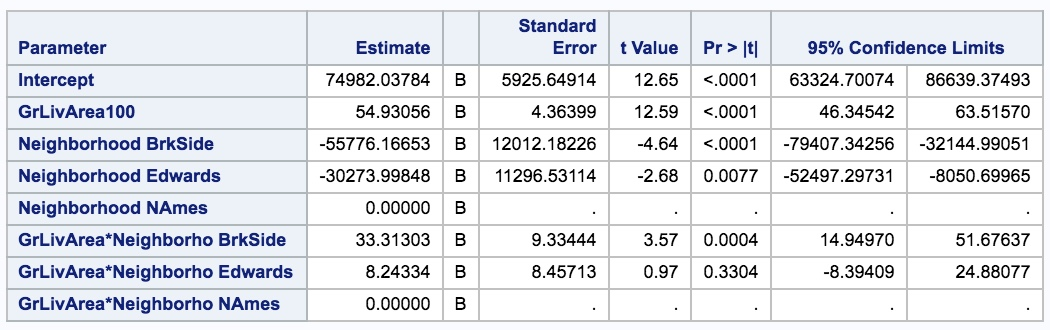
\includegraphics[scale=.3]{../graphics/A1NHcomp}
	\caption{Results of Neighborhood Impact on Sales Price.}
	\label{tab:SMM}
\end{table}
\hrulefill
\begin{table}[H] % [h] forces the table to be output where it is defined in the code (it suppresses floating)
	\centering % Centre the table
	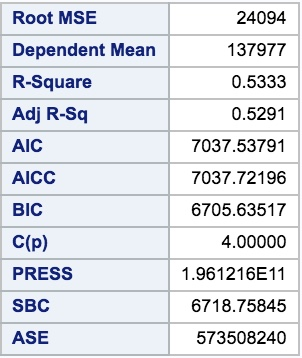
\includegraphics[scale=.4]{../graphics/A1NBMLRResults}
	\caption{Results of Neighborhood Impact on Sales Price.}
	\label{tab:A1Results}
\end{table}
\hrulefill
\begin{table}[H] % [h] forces the table to be output where it is defined in the code (it suppresses floating)
	\centering % Centre the table
	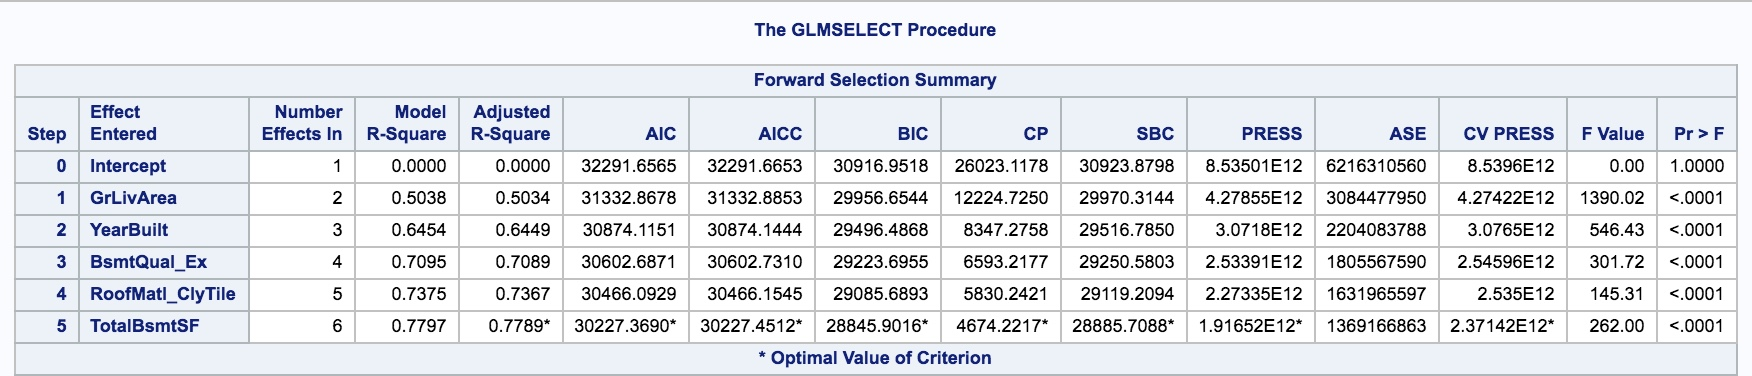
\includegraphics[scale=.25]{../graphics/A2FWfeatures}
	\caption{Forward Selection Model Summary.}
	\label{tab:A2FWsummary}
\end{table}
\hrulefill
\begin{table}[H] % [h] forces the table to be output where it is defined in the code (it suppresses floating)
	\centering % Centre the table
	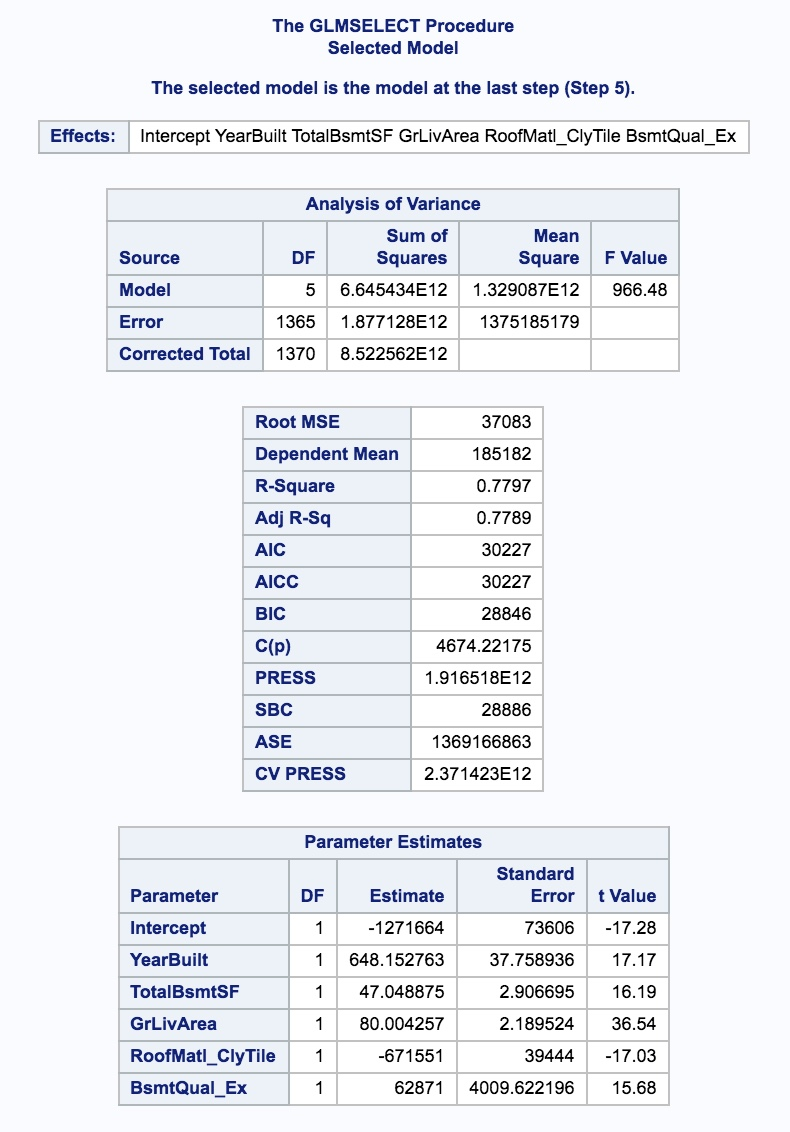
\includegraphics[scale=.3]{../graphics/A2FWresults}
	\caption{Forward Selection Model Performance.}
	\label{tab:A2FWperf}
\end{table}
\hrulefill
\begin{table}[H] % [h] forces the table to be output where it is defined in the code (it suppresses floating)
	\centering % Centre the table
	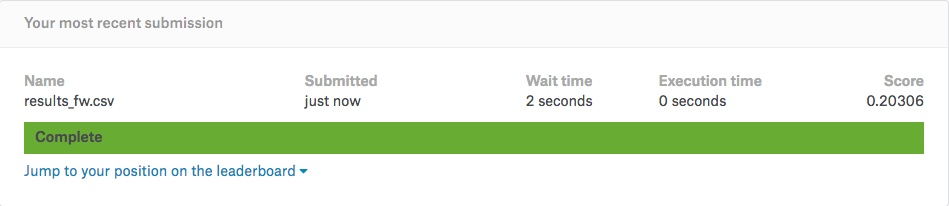
\includegraphics[scale=.4]{../graphics/A2FWKaggle}
	\caption{Forward Selection Model Performance - Kaggle.}
	\label{tab:A2FWKaggle}
\end{table}
\hrulefill
\begin{table}[H] % [h] forces the table to be output where it is defined in the code (it suppresses floating)
	\centering % Centre the table
	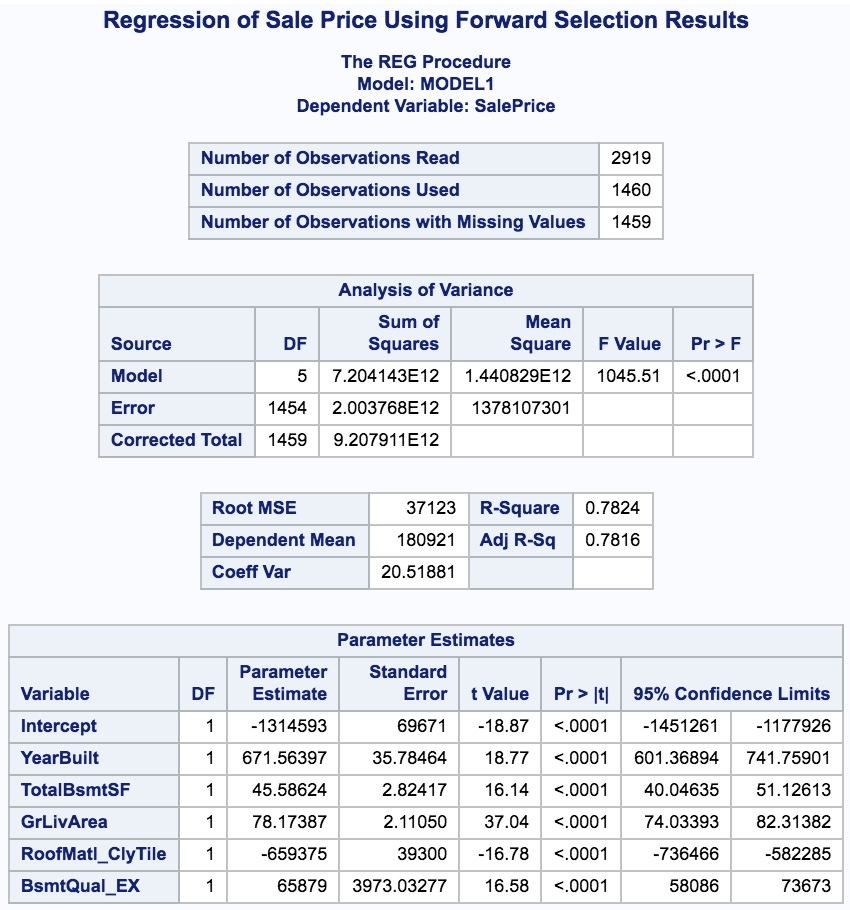
\includegraphics[scale=.3]{../graphics/A2FWCI}
	\caption{Forward Selection Model 95\% Confidence Limits.}
	\label{tab:A2FWCI}
\end{table}
\hrulefill
\begin{table}[H] % [h] forces the table to be output where it is defined in the code (it suppresses floating)
	\centering % Centre the table
	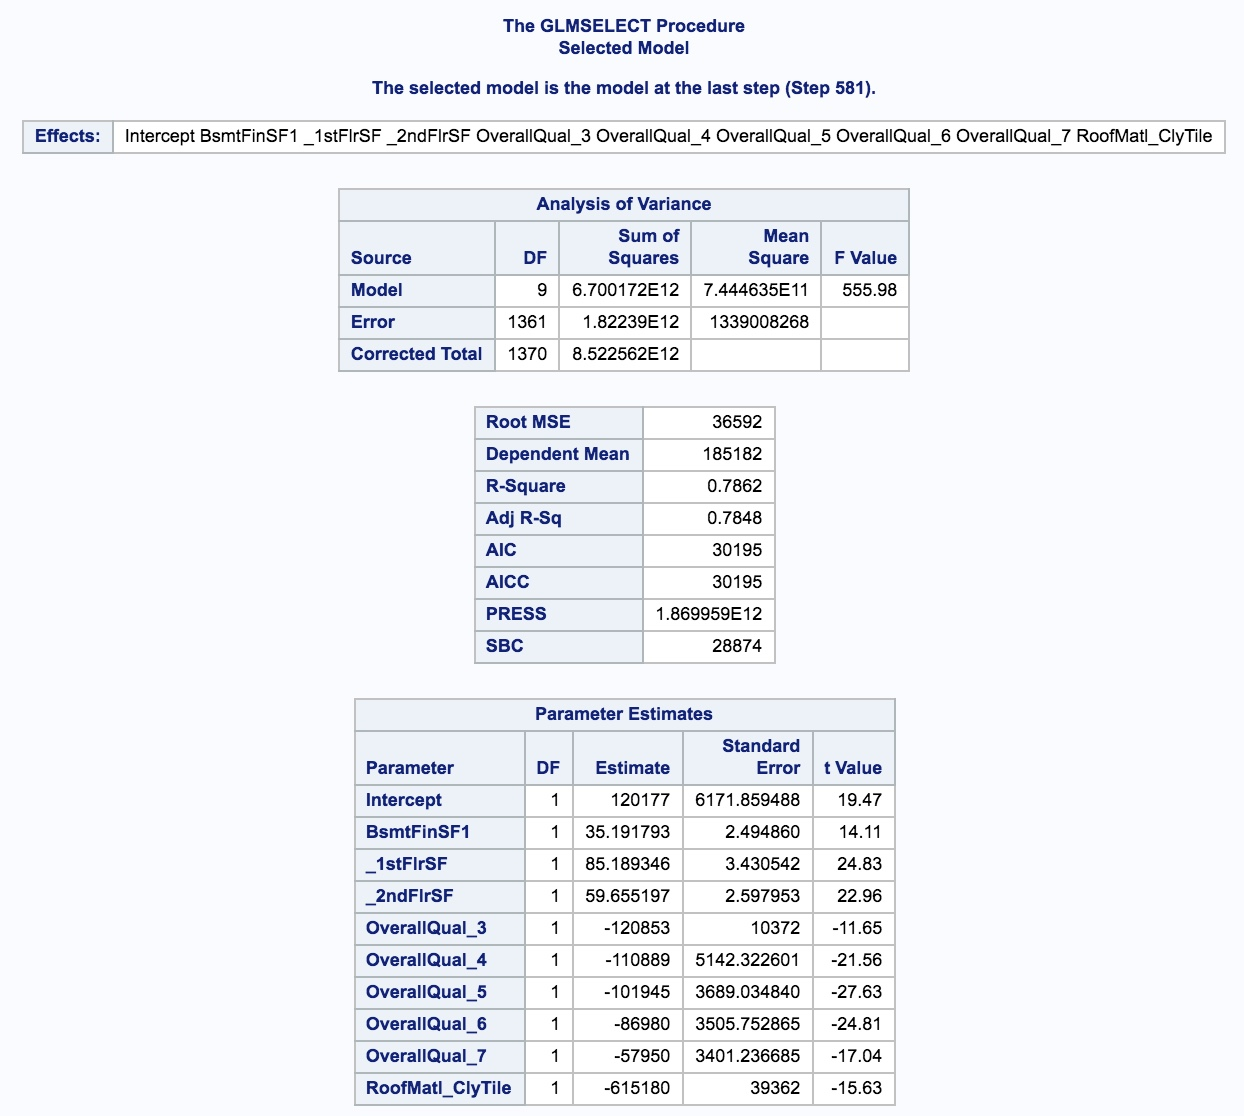
\includegraphics[scale=.3]{../graphics/A2BWresults}
	\caption{Backward Selection Model Performance.}
	\label{tab:A2BWperf}
\end{table}
\hrulefill
\begin{table}[H] % [h] forces the table to be output where it is defined in the code (it suppresses floating)
	\centering % Centre the table
	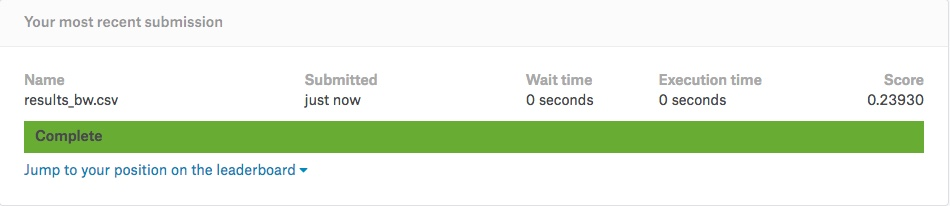
\includegraphics[scale=.4]{../graphics/A2BWKaggle}
	\caption{Backward Selection Model Performance - Kaggle.}
	\label{tab:A2BWKaggle}
\end{table}
\hrulefill
\begin{table}[H] % [h] forces the table to be output where it is defined in the code (it suppresses floating)
	\centering % Centre the table
	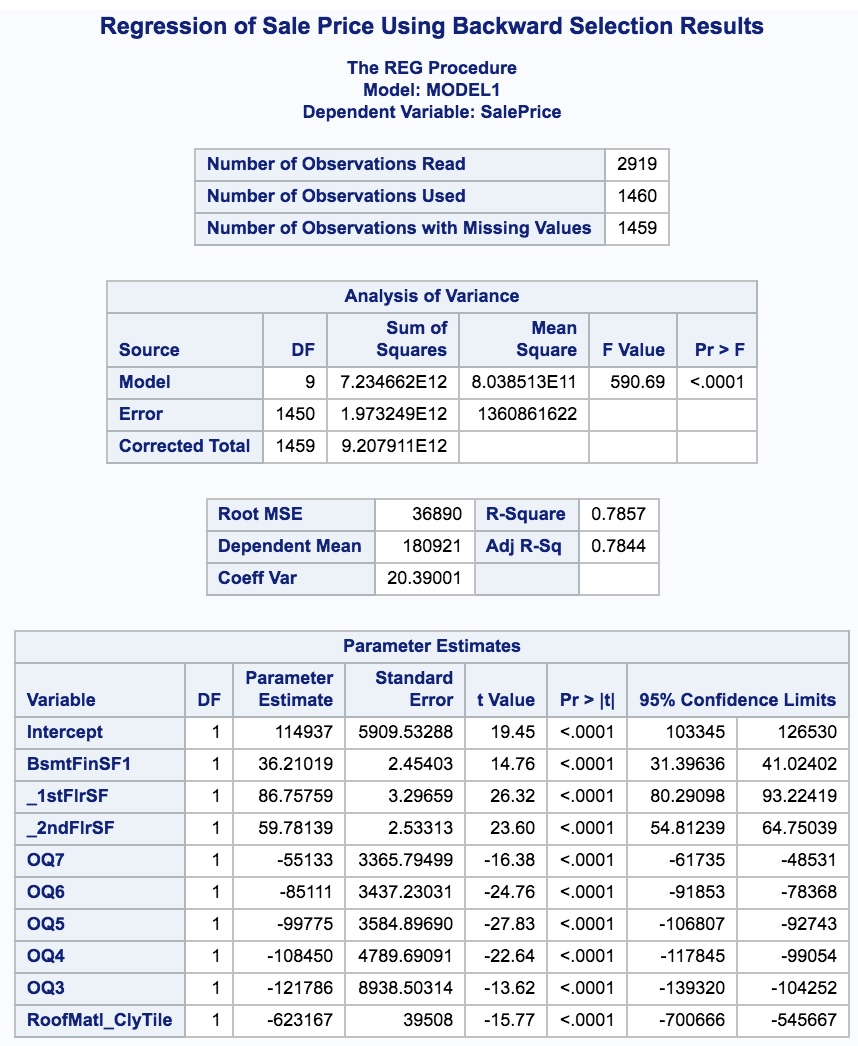
\includegraphics[scale=.3]{../graphics/A2BWCI}
	\caption{Backward Selection Model 95\% Confidence Limits.}
	\label{tab:A2BWCI}
\end{table}
\hrulefill
\begin{table}[H] % [h] forces the table to be output where it is defined in the code (it suppresses floating)
	\centering % Centre the table
	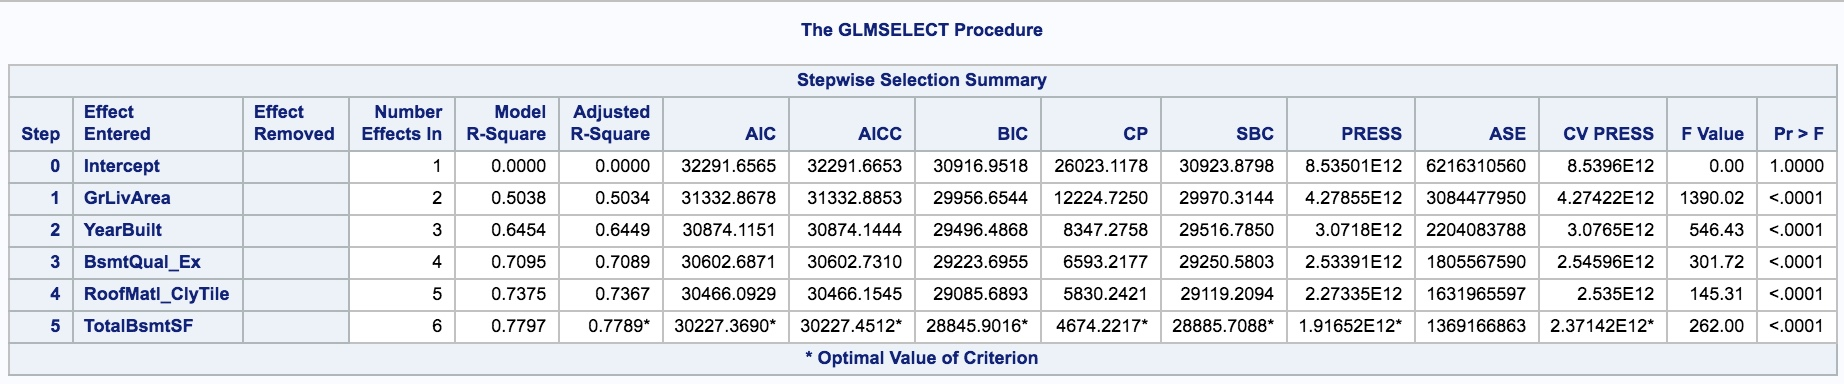
\includegraphics[scale=.25]{../graphics/A2SWfeatures}
	\caption{Stepwise Selection Model Summary.}
	\label{tab:A2SWsummary}
\end{table}
\hrulefill
\begin{table}[H] % [h] forces the table to be output where it is defined in the code (it suppresses floating)
	\centering % Centre the table
	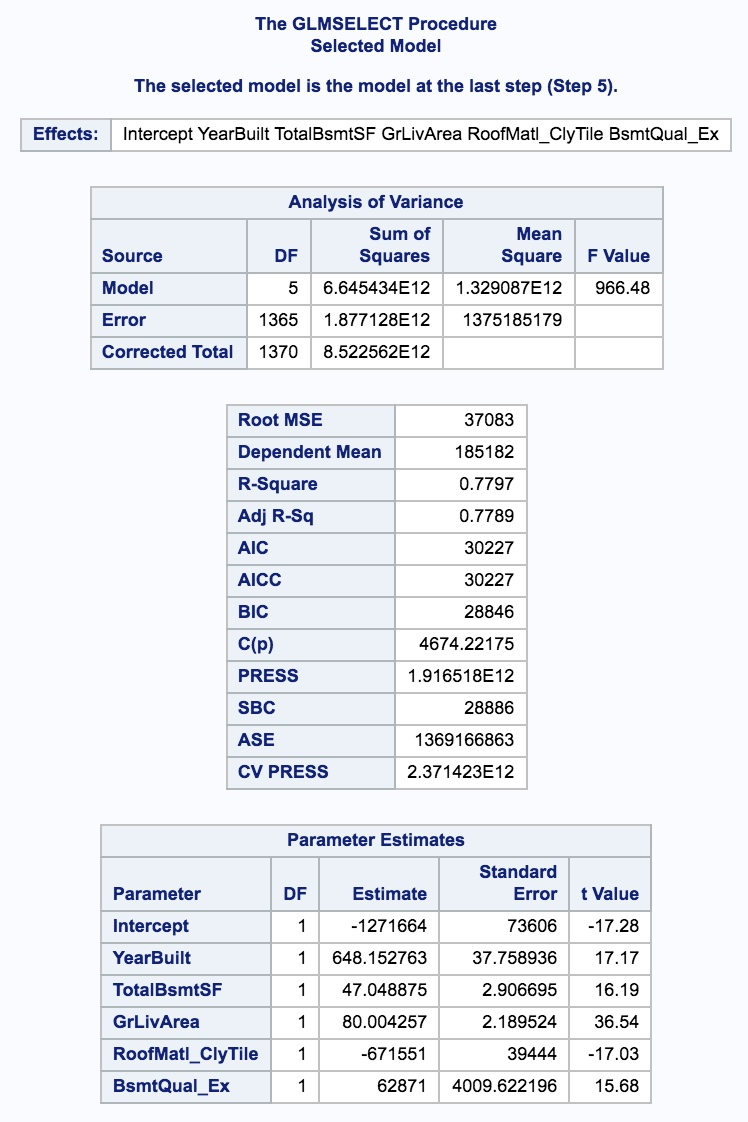
\includegraphics[scale=.3]{../graphics/A2SWresults}
	\caption{Stepwise Selection Model Performance.}
	\label{tab:A2SWperf}
\end{table}
\hrulefill
\begin{table}[H] % [h] forces the table to be output where it is defined in the code (it suppresses floating)
	\centering % Centre the table
	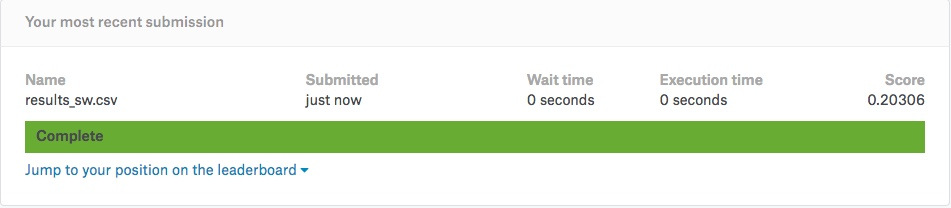
\includegraphics[scale=.4]{../graphics/A2SWKaggle}
	\caption{Stepwise Selection Model Performance - Kaggle.}
	\label{tab:A2SWKaggle}
\end{table}
\hrulefill
\begin{table}[H] % [h] forces the table to be output where it is defined in the code (it suppresses floating)
	\centering % Centre the table
	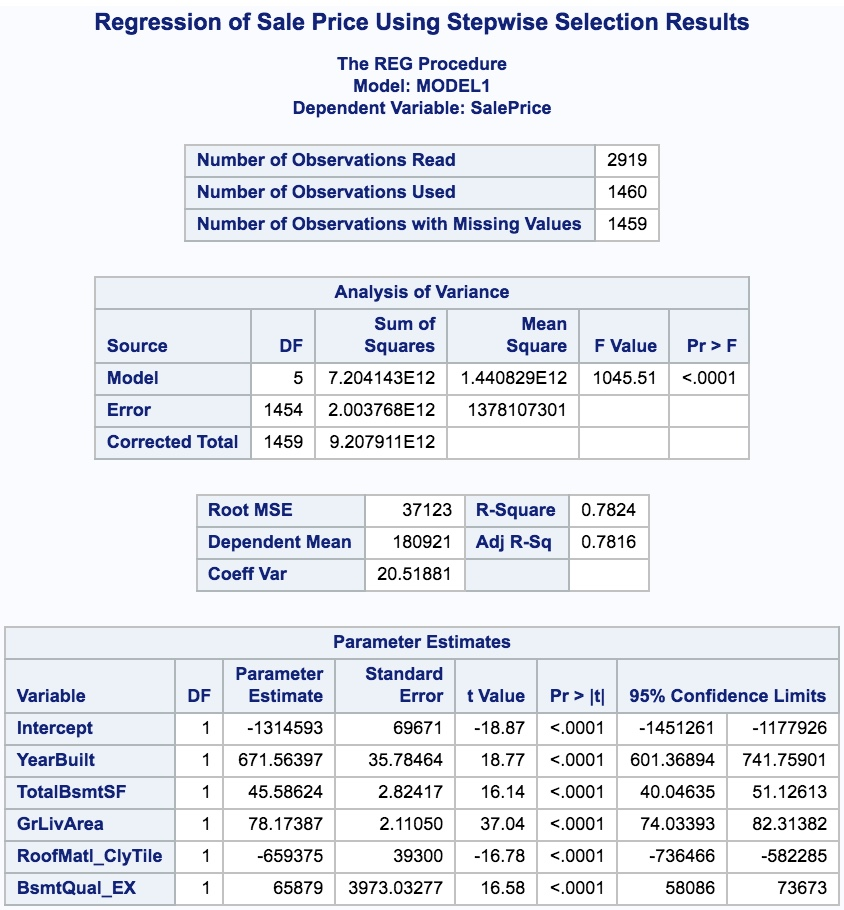
\includegraphics[scale=.3]{../graphics/A2SWCI}
	\caption{Stepwise Selection Model 95\% Confidence Limits.}
	\label{tab:A2SWCI}
\end{table}
\hrulefill
\pagebreak

\section{List of Figures}
\label{sec:Figures}
\begin{figure}[H] % [h] forces the figure to be output where it is defined in the code (it suppresses floating)
	\centering
	\begin{tabular}{p{0.48\textwidth} p{0.48\textwidth}}
	\hline
	\multicolumn{1}{|c|}{Original} & \multicolumn{1}{|c|}{After Removal of Outliers} \\
		\multicolumn{1}{|c|}{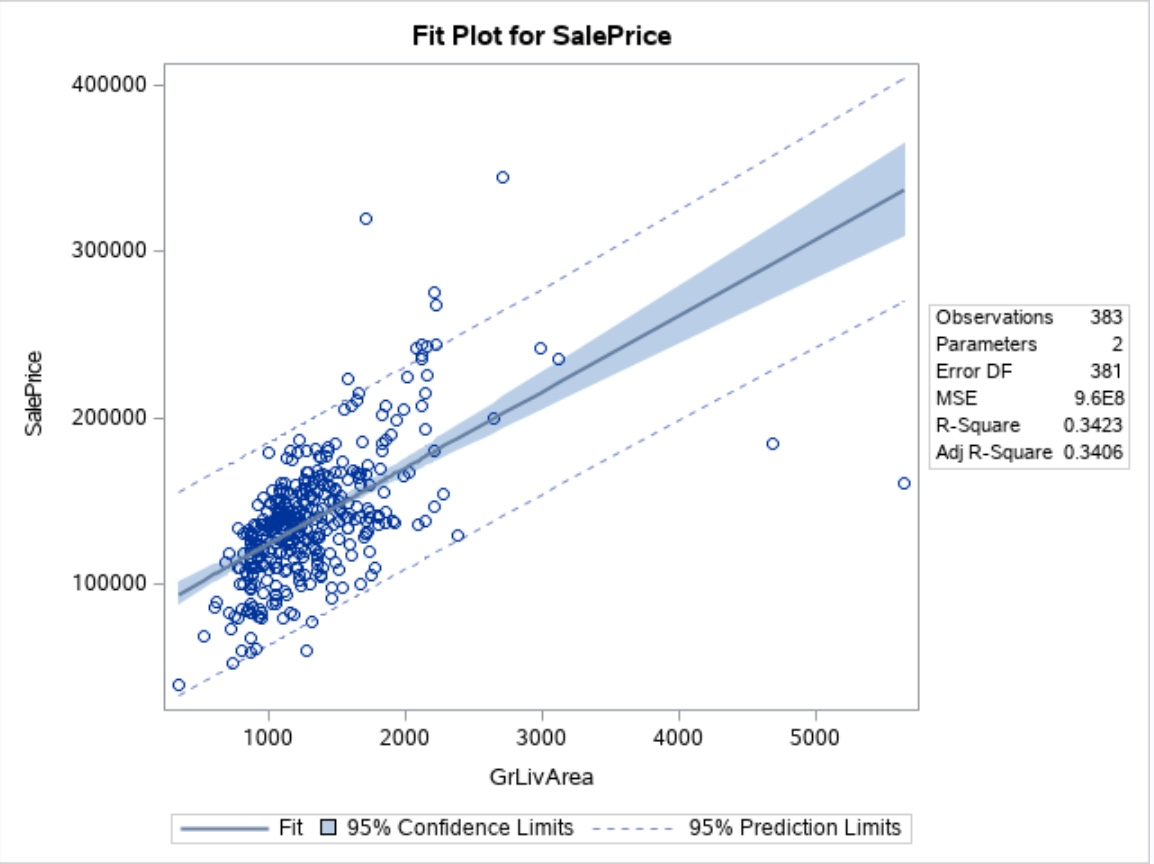
\includegraphics[width=0.48\textwidth]{../graphics/A1LR1}} &
		\multicolumn{1}{|c|}{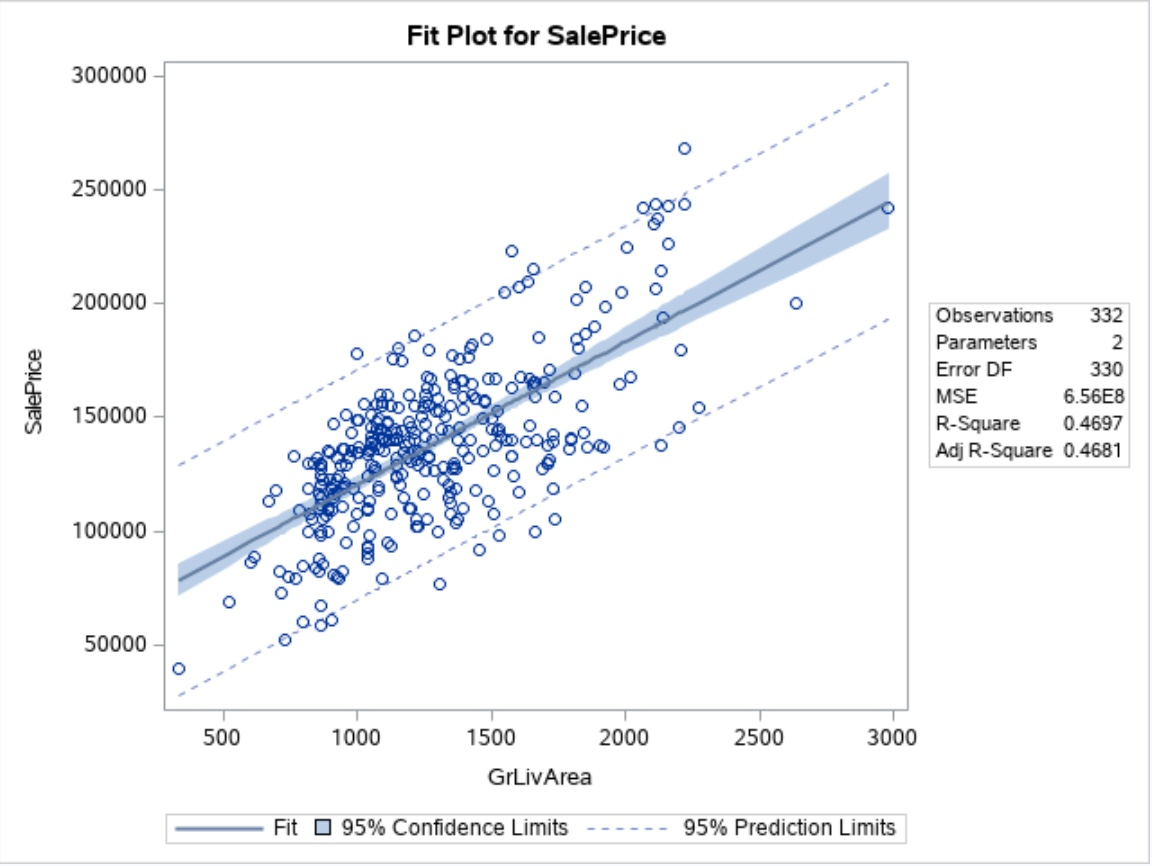
\includegraphics[width=0.48\textwidth]{../graphics/A1LR2}}\\
		\hline
	\end{tabular}		
	\caption{Simple Linear Regression Models.}
	\label{fig:A1LR}
\end{figure}
\begin{figure}[H] % [h] forces the figure to be output where it is defined in the code (it suppresses floating)
	\centering
	\begin{tabular}{p{0.23\textwidth} p{0.23\textwidth}p{0.23\textwidth}p{0.23\textwidth}}
\hline	
	\multicolumn{2}{|c|}{Original} &  \multicolumn{2}{|c|}{After Removal of Outliers} \\
		\multicolumn{1}{|c}{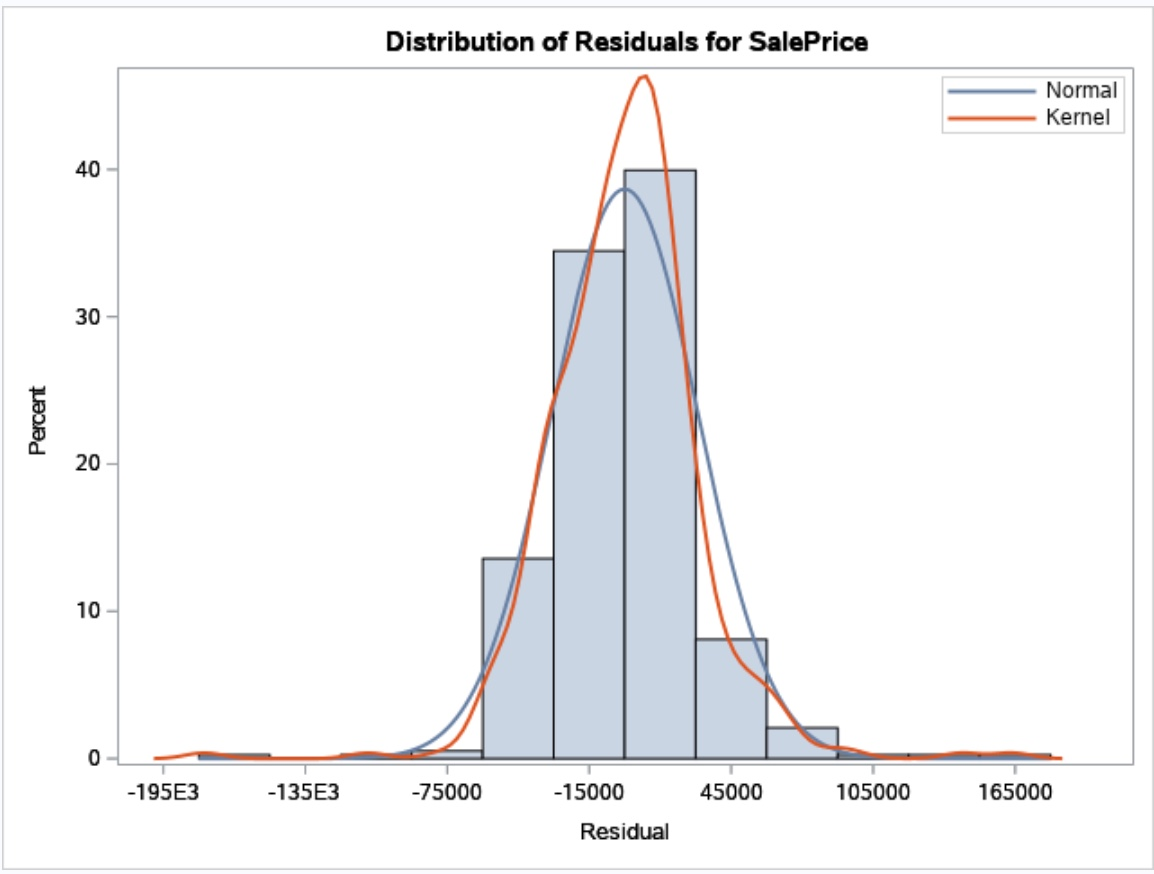
\includegraphics[width=0.23\textwidth]{../graphics/A1Norm1}} &
		\multicolumn{1}{c|}{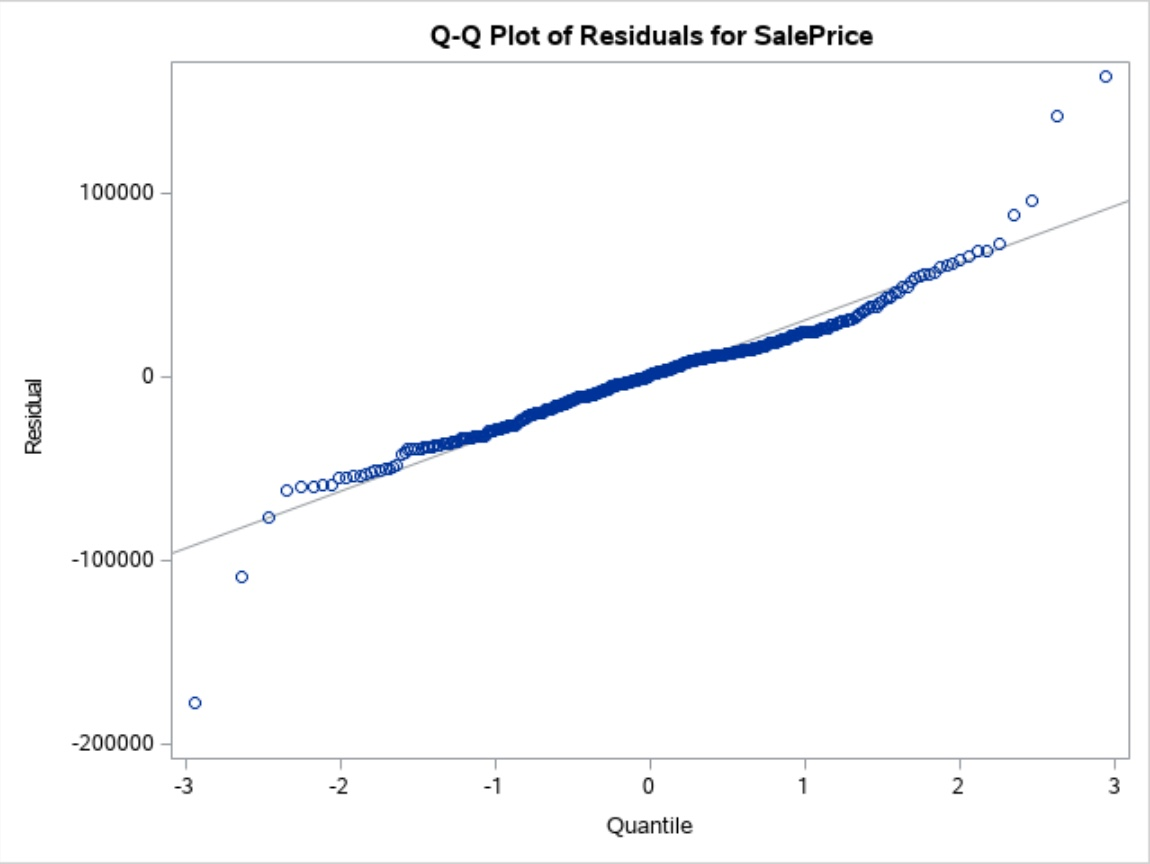
\includegraphics[width=0.23\textwidth]{../graphics/A1qq1}} &
		\multicolumn{1}{|c}{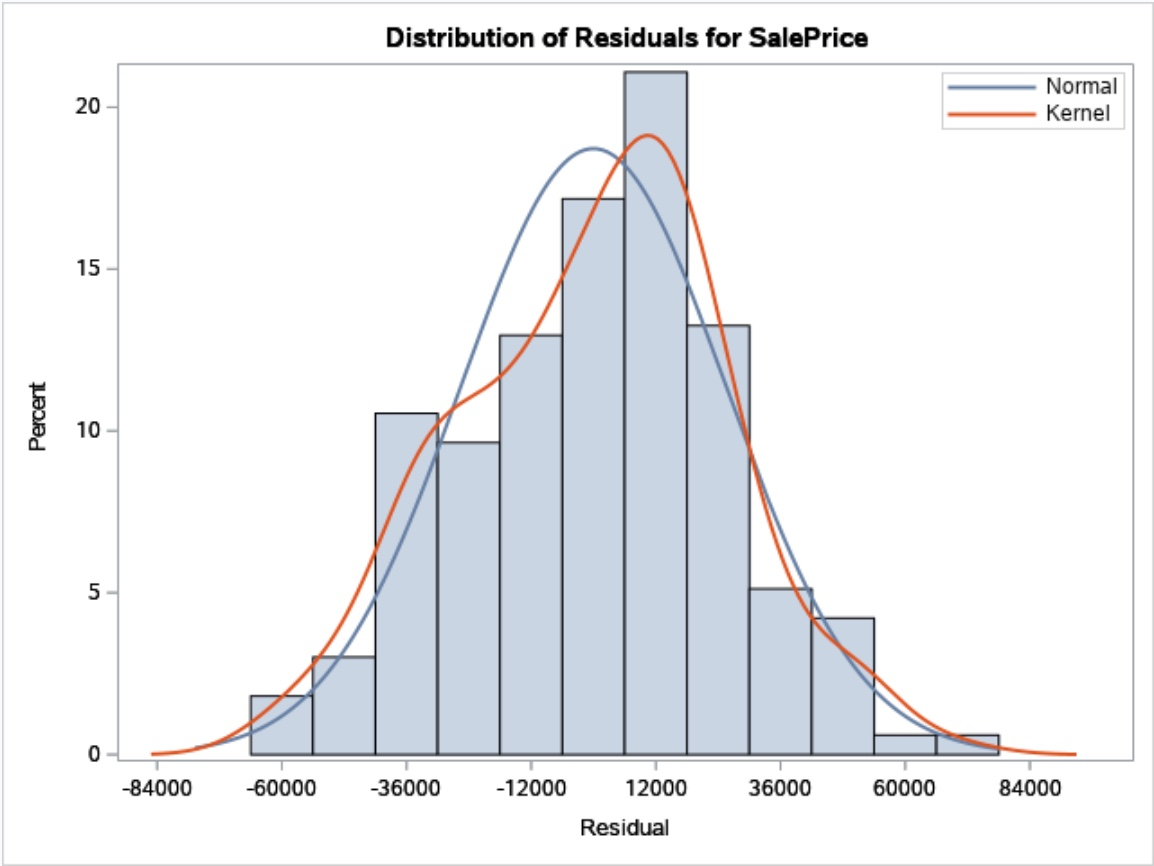
\includegraphics[width=0.23\textwidth]{../graphics/A1Norm2}} &
		\multicolumn{1}{c|}{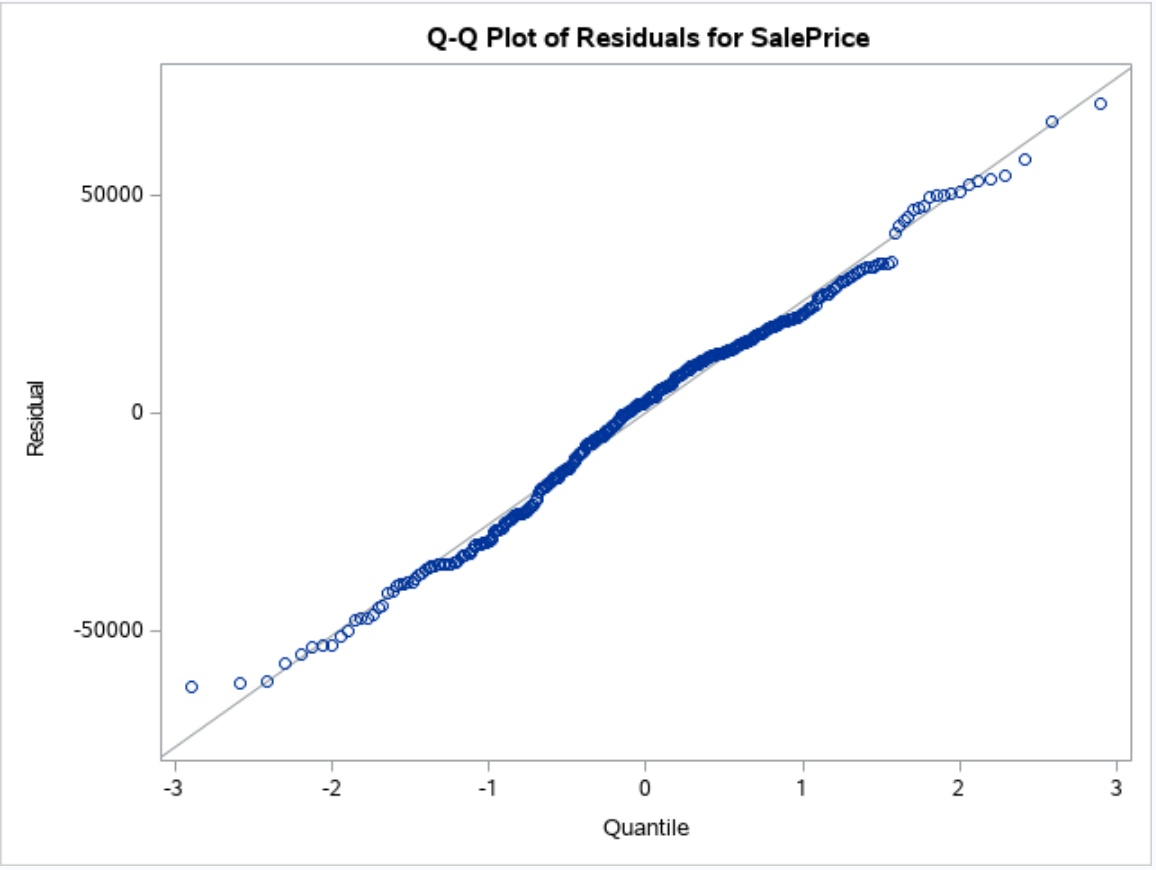
\includegraphics[width=0.23\textwidth]{../graphics/A1qq2}}\\
		\hline
	\end{tabular}		
	\caption{Normality Plots.}
	\label{fig:A1QQ}
\end{figure}
\begin{figure}[H] % [h] forces the figure to be output where it is defined in the code (it suppresses floating)
	\centering
	\begin{tabular}{p{0.23\textwidth} p{0.23\textwidth}p{0.23\textwidth}p{0.23\textwidth}}
	\hline
	\multicolumn{2}{|c|}{Original} &  \multicolumn{2}{|c|}{After Removal of Outliers} \\
		\multicolumn{1}{|c}{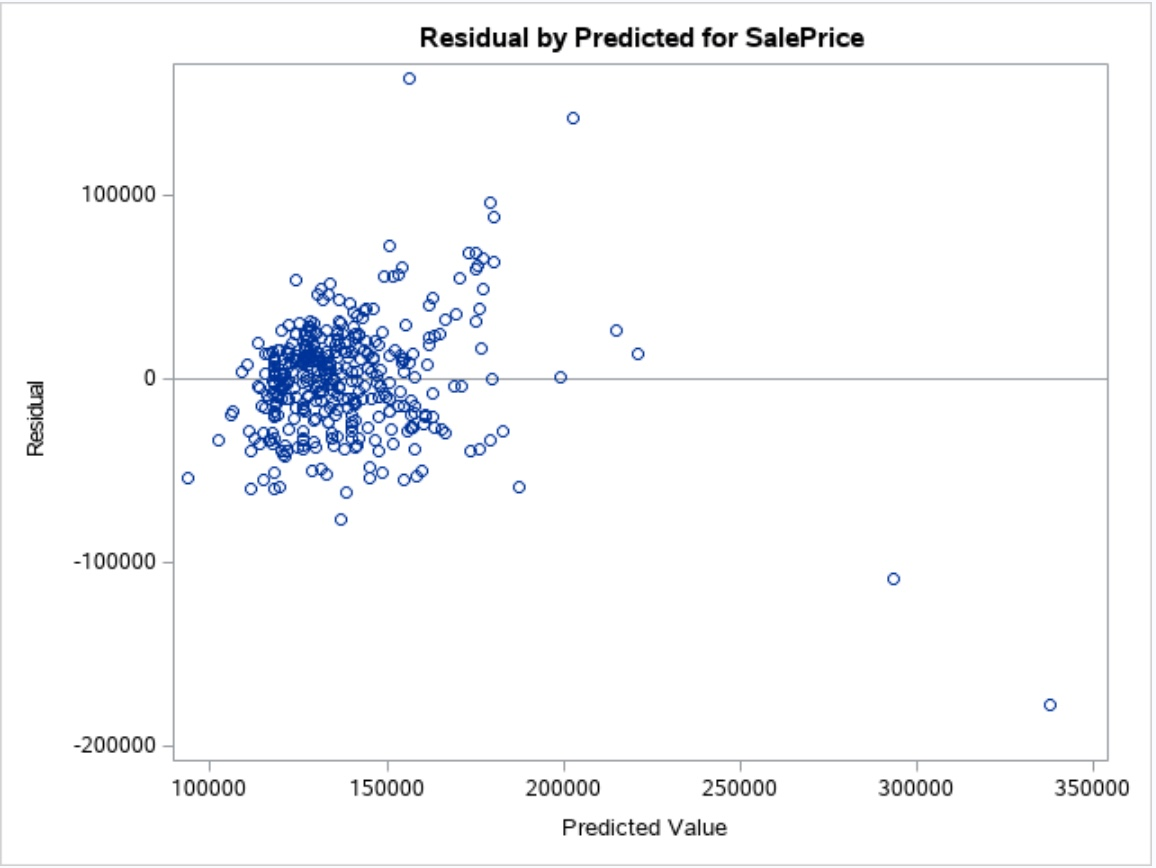
\includegraphics[width=0.23\textwidth]{../graphics/A1Residuals1}} &
		\multicolumn{1}{c|}{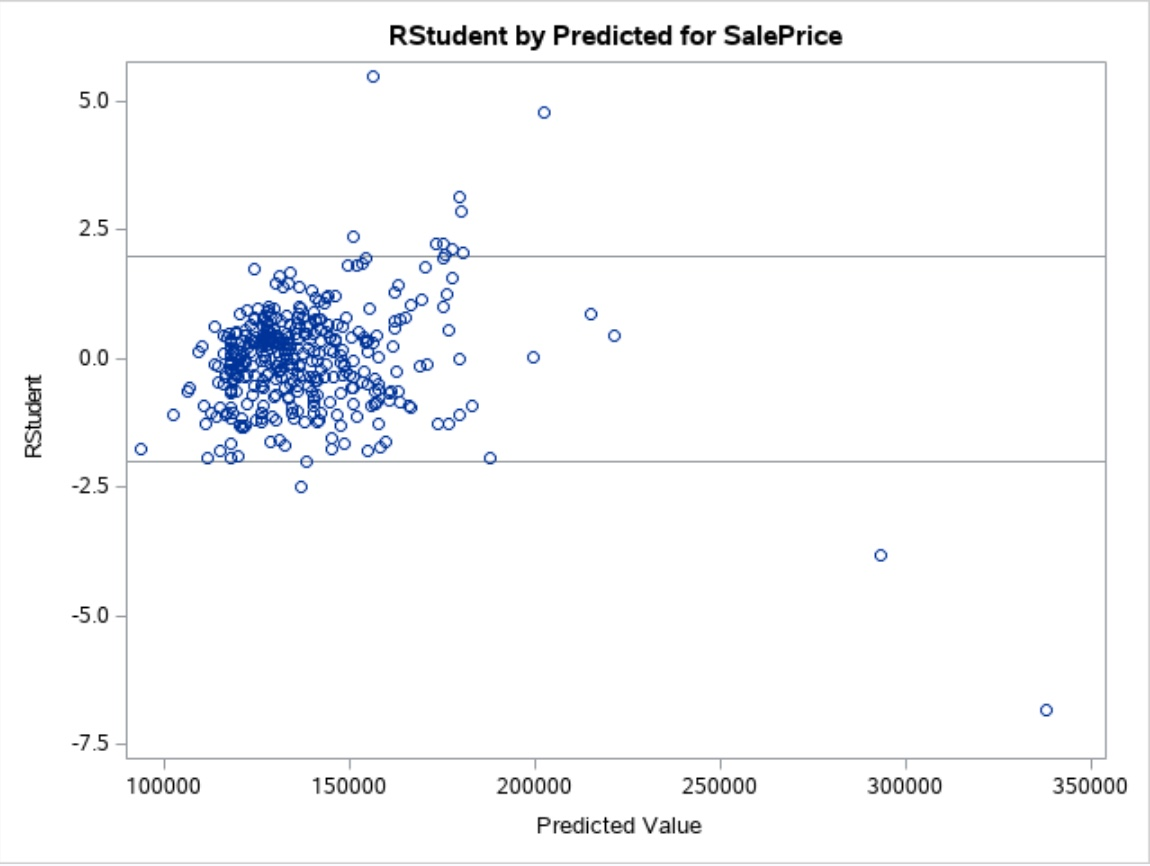
\includegraphics[width=0.23\textwidth]{../graphics/A1StudentResiduals1}} &
		\multicolumn{1}{|c}{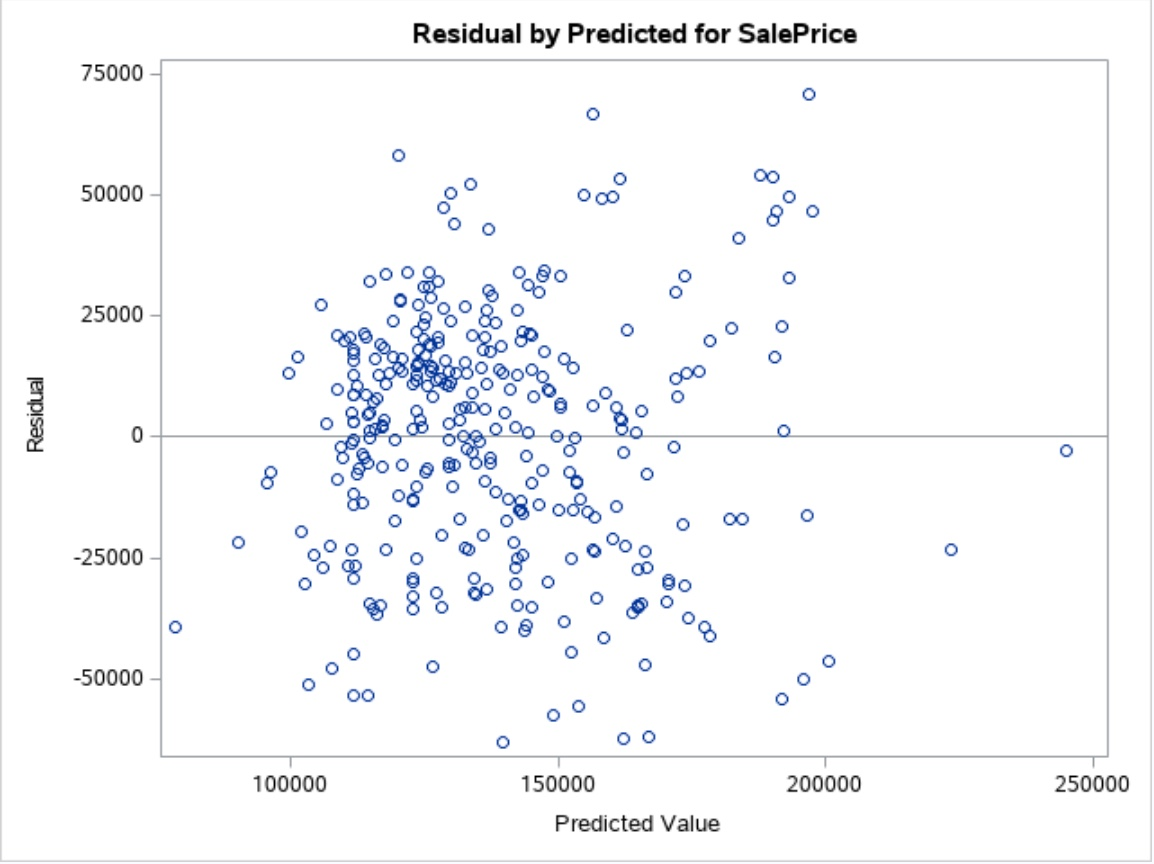
\includegraphics[width=0.23\textwidth]{../graphics/A1Residuals2}} &
		\multicolumn{1}{c|}{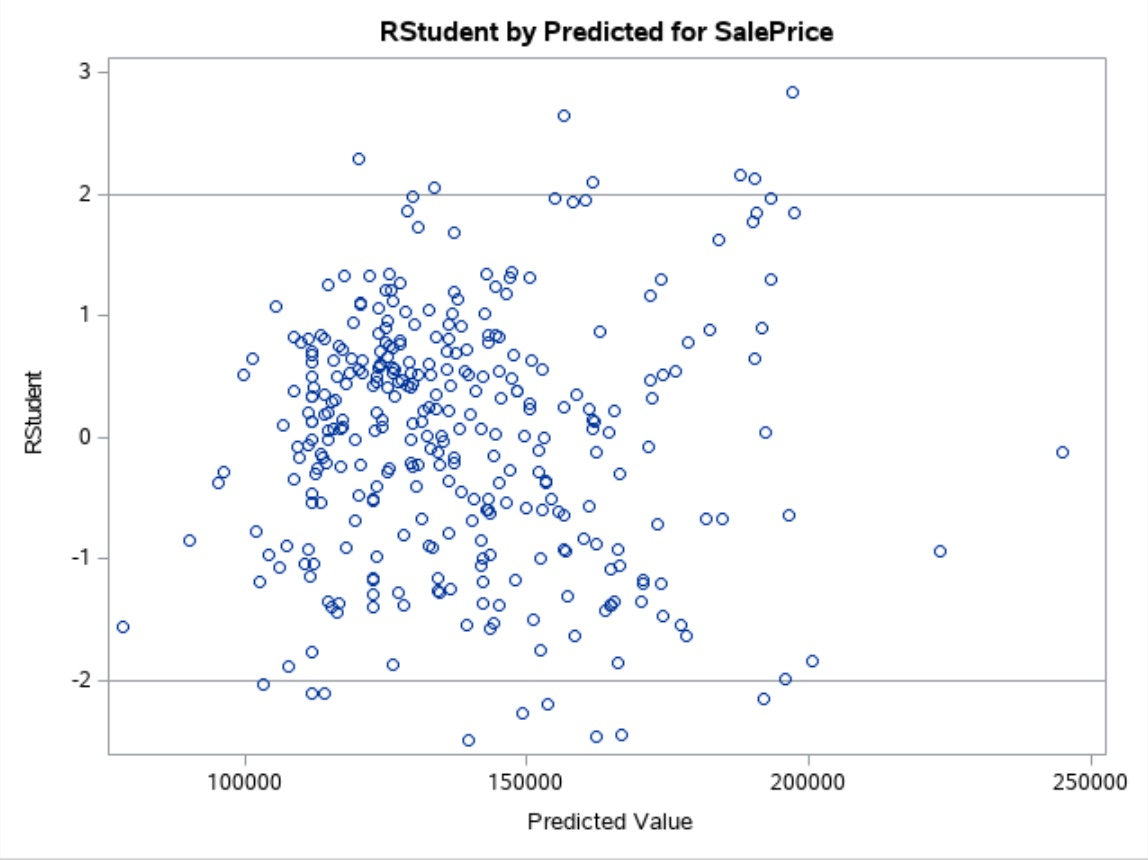
\includegraphics[width=0.23\textwidth]{../graphics/A1StudentResiduals2}}\\
		\hline
	\end{tabular}		
	\caption{Residual Plots.}
	\label{fig:A1RP}
\end{figure}
\begin{figure}[H] % [h] forces the figure to be output where it is defined in the code (it suppresses floating)
	\centering
	\begin{tabular}{p{0.23\textwidth} p{0.23\textwidth}p{0.23\textwidth}p{0.23\textwidth}}
\hline	
	\multicolumn{2}{|c|}{Original} &  \multicolumn{2}{|c|}{After Removal of Outliers} \\
		\multicolumn{1}{|c}{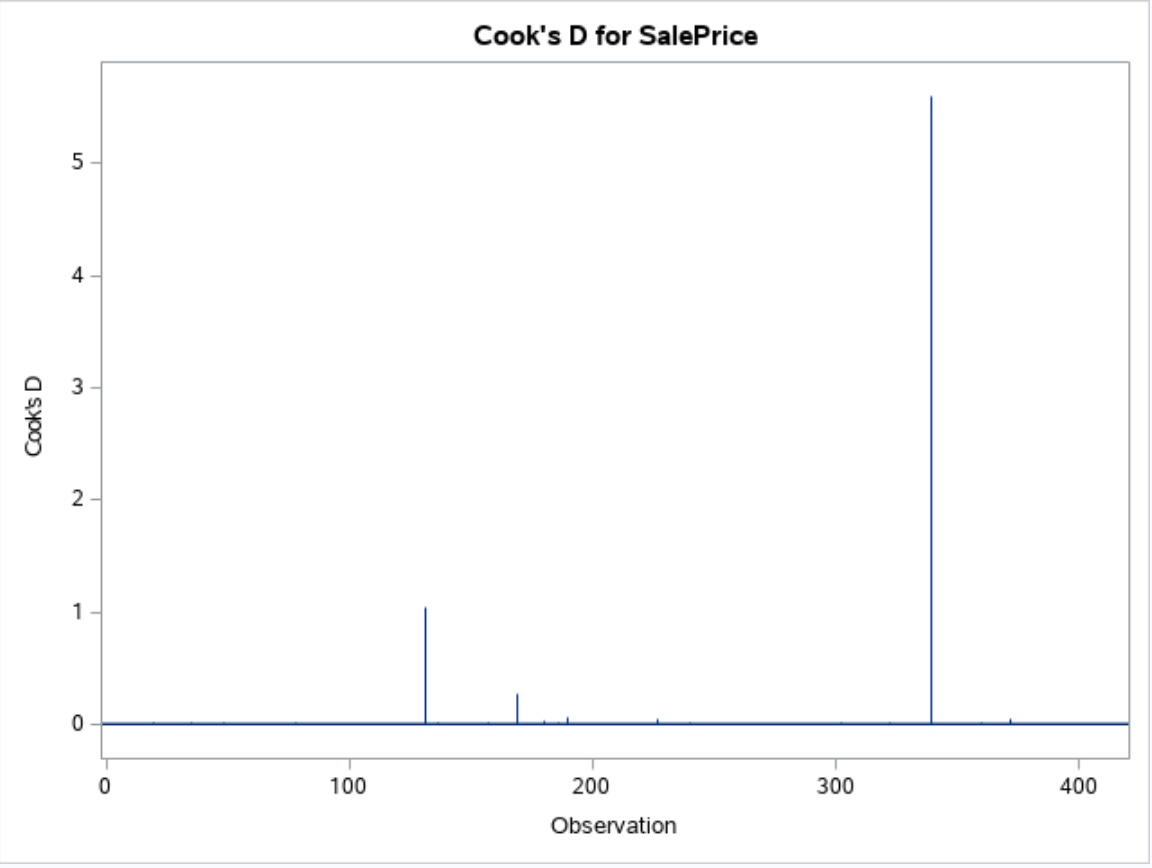
\includegraphics[width=0.23\textwidth]{../graphics/A1Cooks1}} &
		\multicolumn{1}{c|}{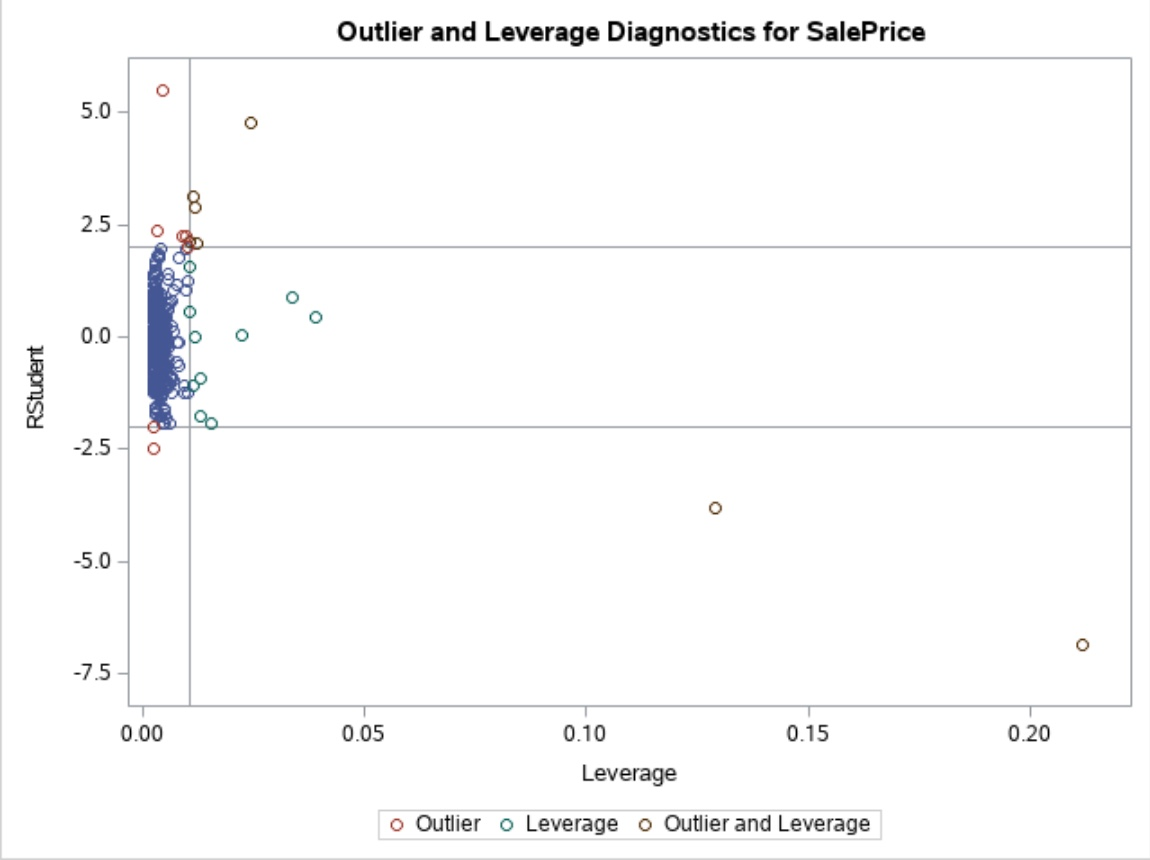
\includegraphics[width=0.23\textwidth]{../graphics/A1Lev1}} &
		\multicolumn{1}{|c}{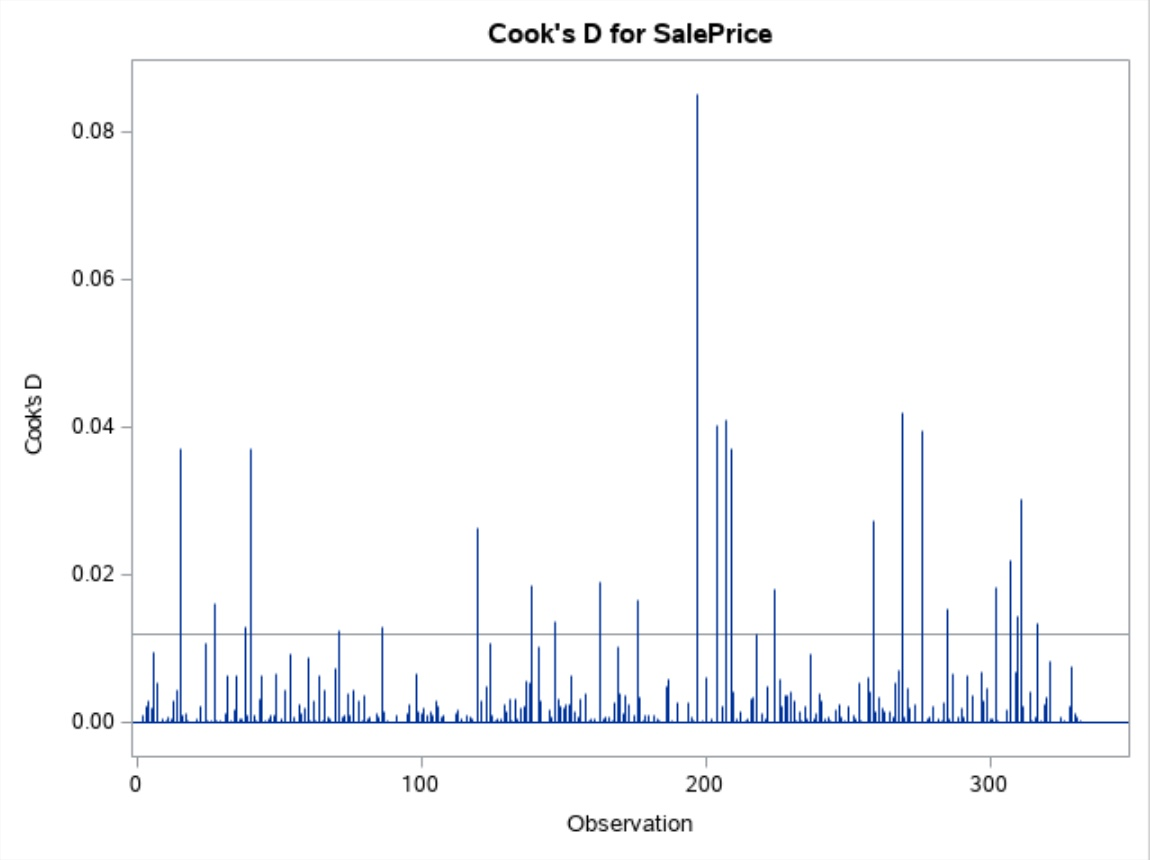
\includegraphics[width=0.23\textwidth]{../graphics/A1Cooks2}} &
		\multicolumn{1}{c|}{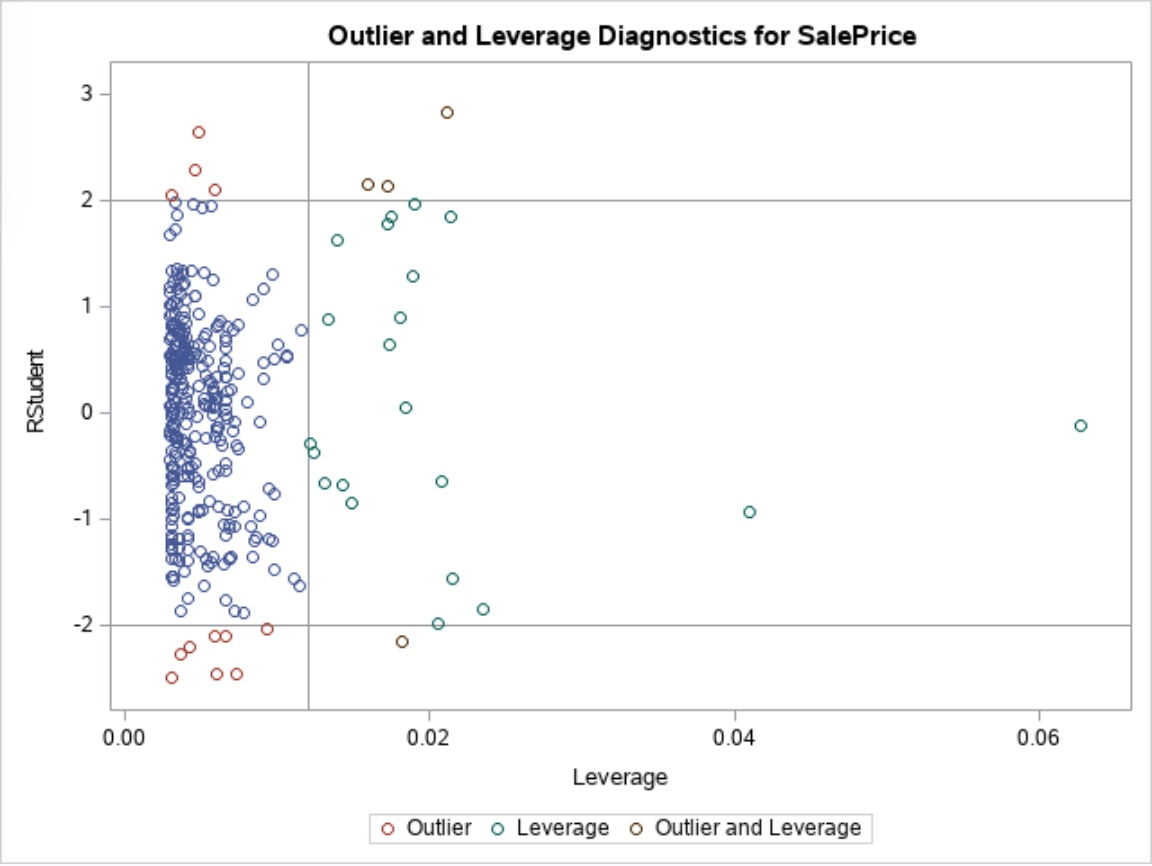
\includegraphics[width=0.23\textwidth]{../graphics/A1Lev2}}\\
		\hline
	\end{tabular}		
	\caption{Influential Point Plots.}
	\label{fig:A1IP}
\end{figure}
\begin{figure}[H] % [h] forces the figure to be output where it is defined in the code (it suppresses floating)
	\centering
	\begin{tabular}{p{0.48\textwidth} p{0.48\textwidth}}
\hline	
	\multicolumn{1}{|c|}{Original} &  \multicolumn{1}{|c|}{After Removal of Outliers} \\
		\multicolumn{1}{|c|}{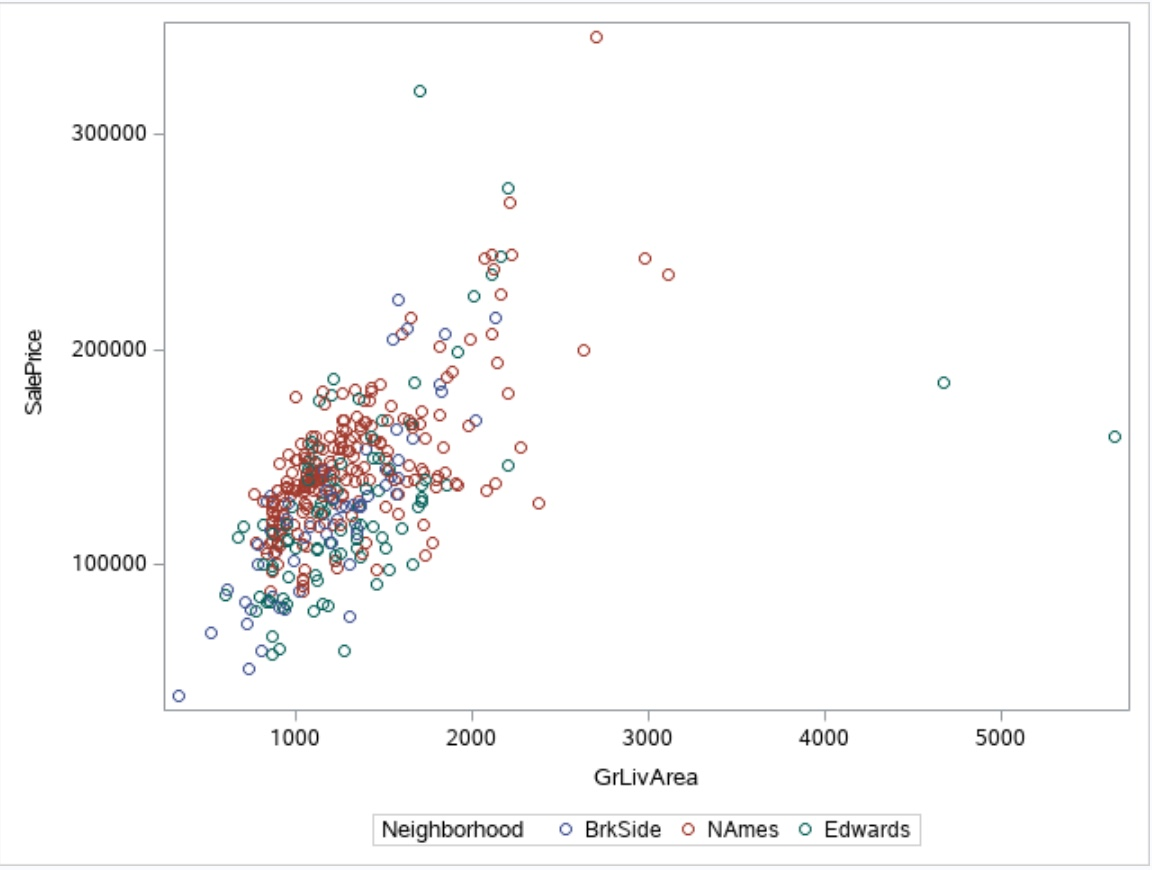
\includegraphics[width=0.48\textwidth]{../graphics/A1NHscat1}} &
		\multicolumn{1}{|c|}{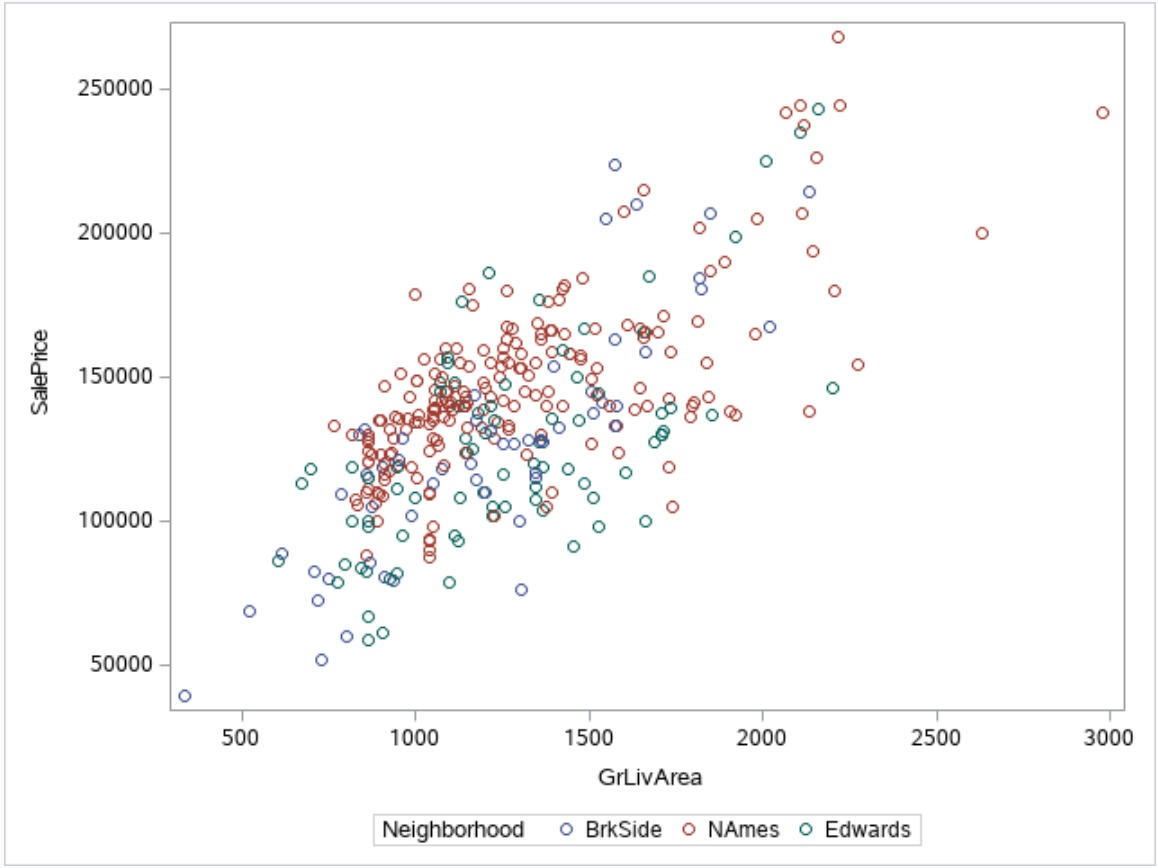
\includegraphics[width=0.48\textwidth]{../graphics/A1NHscat2}}\\
		\hline
	\end{tabular}		
	\caption{Scatterplot of Sale Prices vs Living Area by Neighborhood.}
	\label{fig:NBscat}
\end{figure}
\begin{figure}[H] % [h] forces the figure to be output where it is defined in the code (it suppresses floating)
	\centering
	\begin{tabular}{| p{0.95\textwidth}|}
	\hline
	\\
	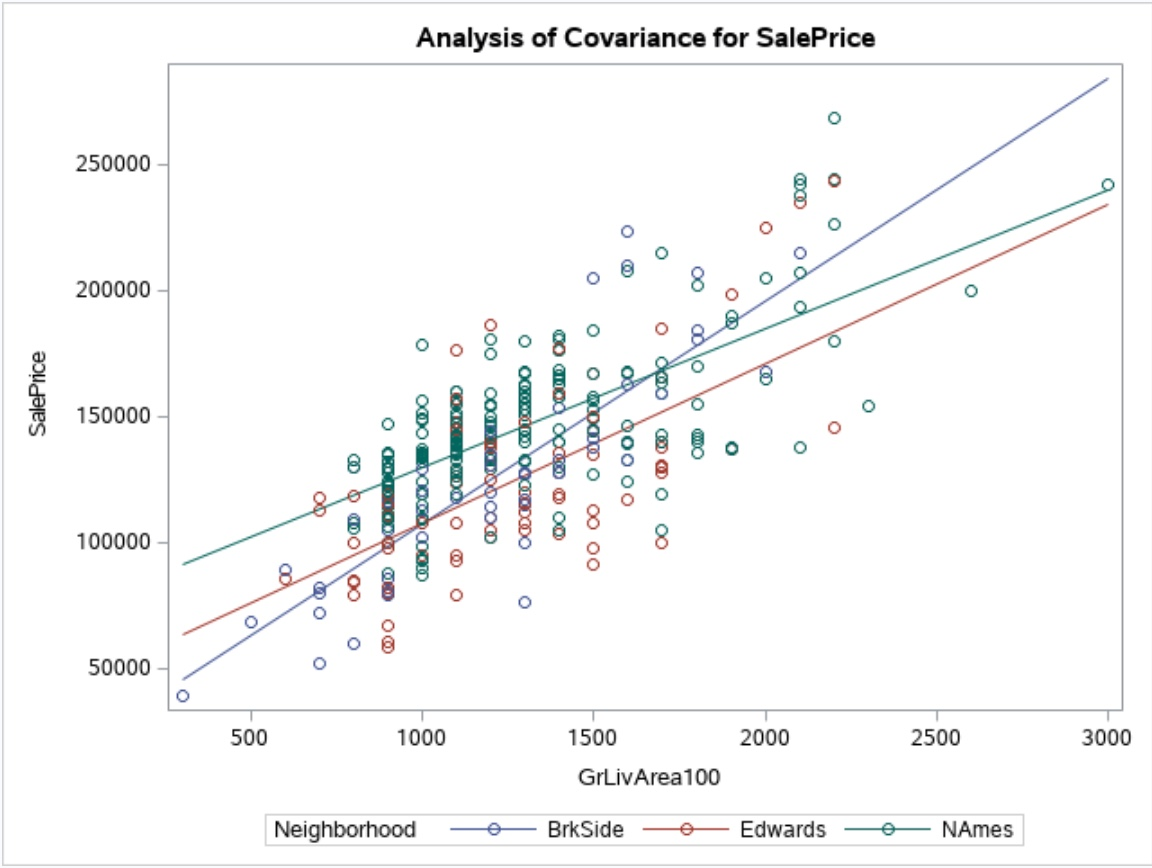
\includegraphics[width=0.95\textwidth]{../graphics/A1NBMLR}\\
	\hline
	\end{tabular}	
	\caption{Linear Regression Model by Neighborhood.}
	\label{fig:NBLRM}
\end{figure}
\begin{figure}[H] % [h] forces the figure to be output where it is defined in the code (it suppresses floating)
	\centering
	\begin{tabular}{| p{0.60\textwidth}|}
	\hline
	\\
	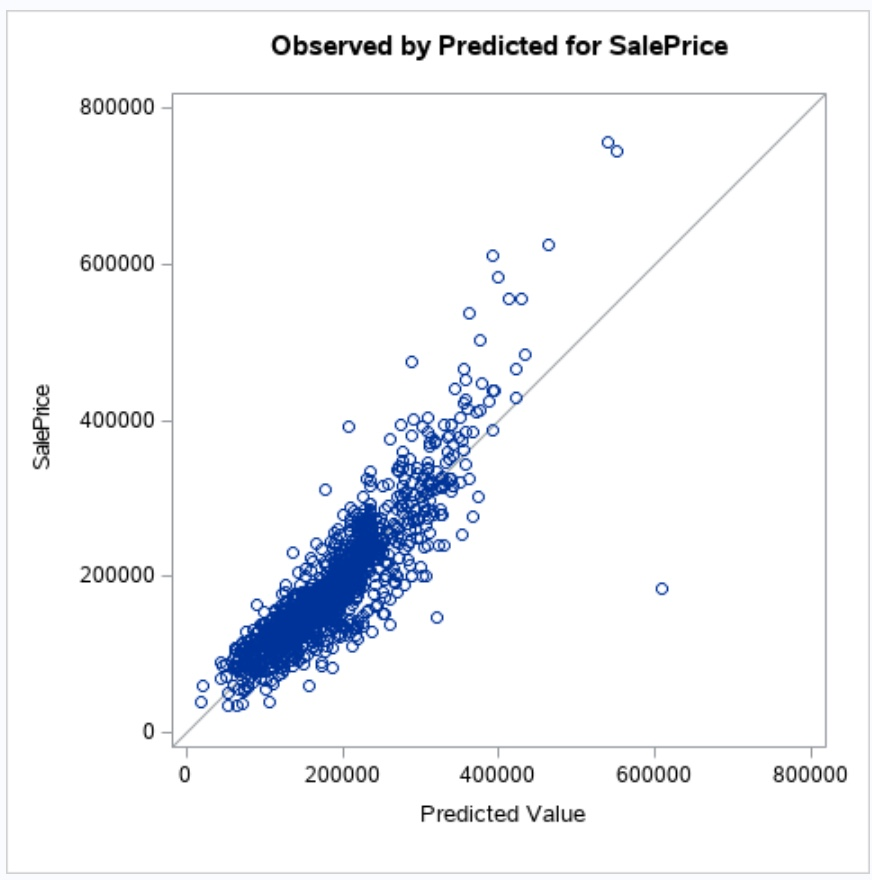
\includegraphics[width=0.60\textwidth]{../graphics/A2FWscatt}\\
	\hline
	\end{tabular}	
	\caption{Scatter Plot Forward Selection Model.}
	\label{fig:A2FWscatt}
\end{figure}
\begin{figure}[H] % [h] forces the figure to be output where it is defined in the code (it suppresses floating)
	\centering
	\begin{tabular}{p{0.48\textwidth} p{0.48\textwidth}}
	\hline
	\multicolumn{1}{|c}{} &  \multicolumn{1}{c|}{} \\
		\multicolumn{1}{|c}{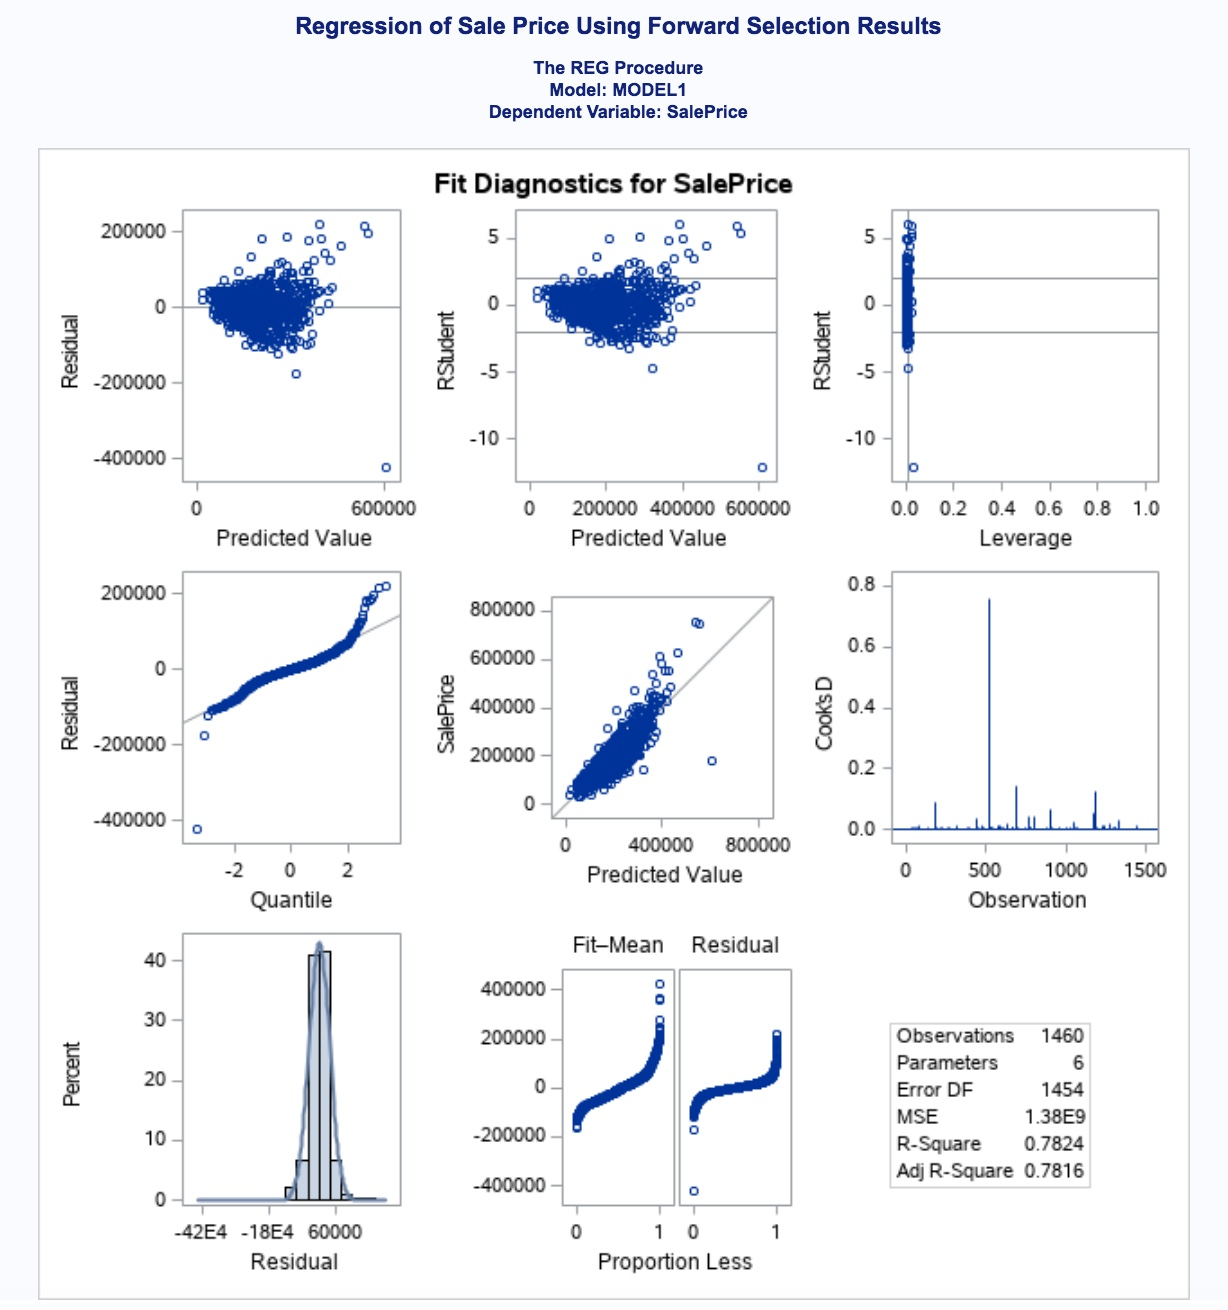
\includegraphics[width=0.48\textwidth]{../graphics/A2FWAss1}} &
		\multicolumn{1}{c|}{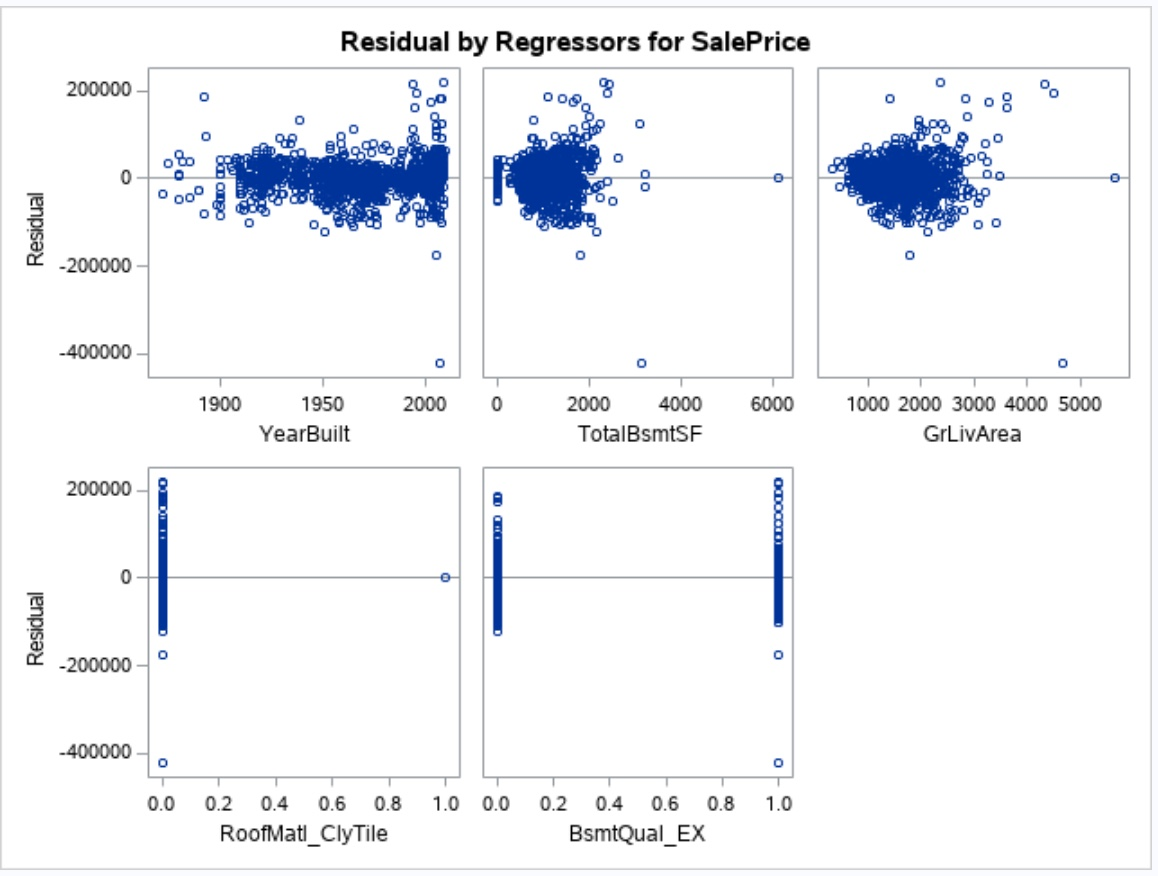
\includegraphics[width=0.48\textwidth]{../graphics/A2FWAss2}}\\
		\hline
	\end{tabular}		
	\caption{Plots for Forward Selection Model.}
	\label{fig:A2FWAss}
\end{figure}
\begin{figure}[H] % [h] forces the figure to be output where it is defined in the code (it suppresses floating)
	\centering
	\begin{tabular}{p{0.48\textwidth} p{0.48\textwidth}}
\hline	
	\multicolumn{1}{|c}{} &  \multicolumn{1}{c|}{} \\
		\multicolumn{1}{|c}{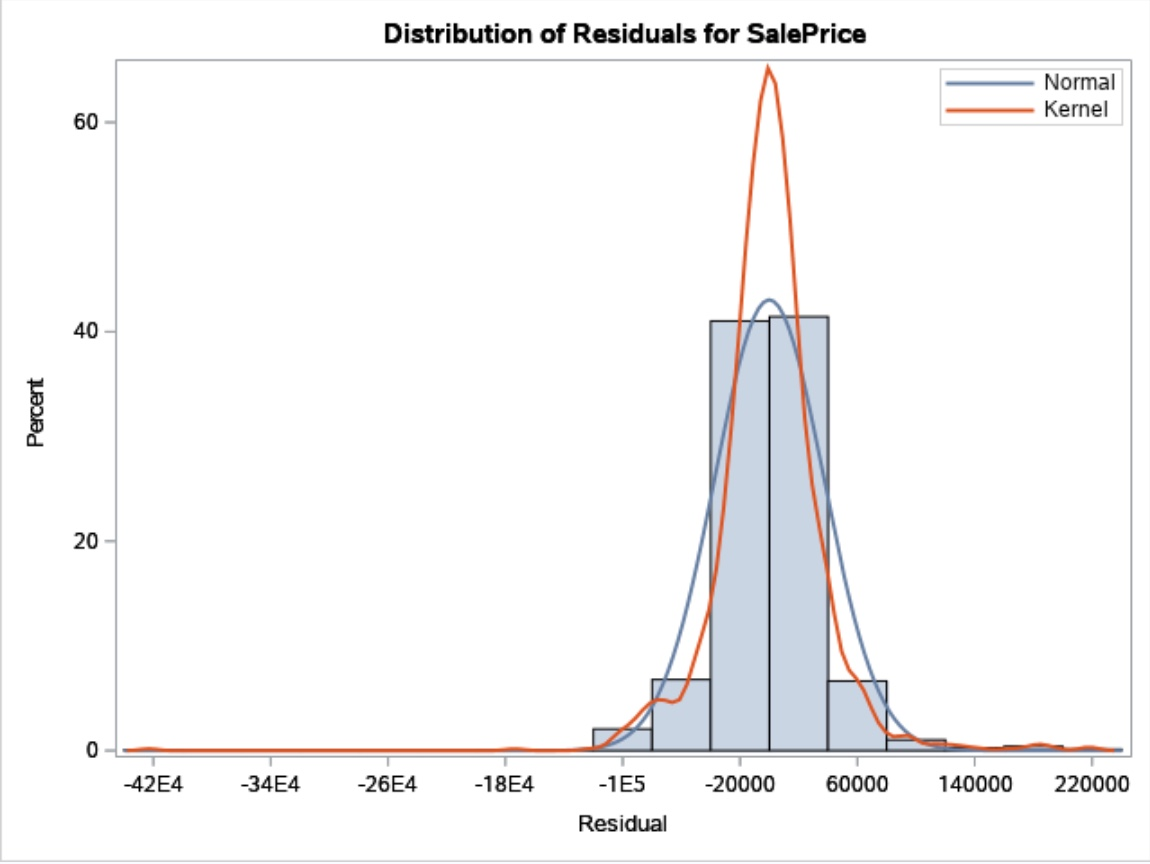
\includegraphics[width=0.48\textwidth]{../graphics/A2FWHist}} &
		\multicolumn{1}{c|}{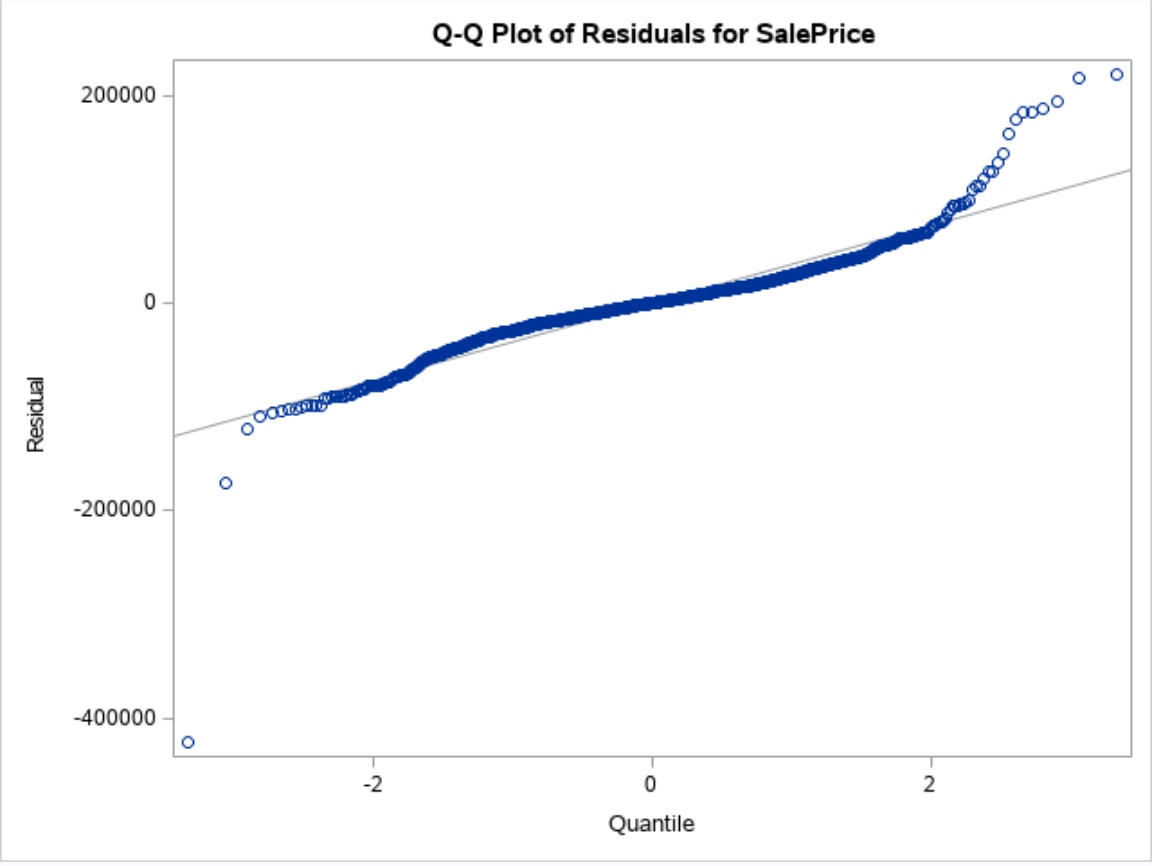
\includegraphics[width=0.48\textwidth]{../graphics/A2FWqq}}\\
		\hline
	\end{tabular}		
	\caption{Normality Plots for Forward Selection Model.}
	\label{fig:A2FWQQ}
\end{figure}
\begin{figure}[H] % [h] forces the figure to be output where it is defined in the code (it suppresses floating)
	\centering
	\begin{tabular}{p{0.48\textwidth} p{0.48\textwidth}}
\hline	
	\multicolumn{1}{|c}{} &  \multicolumn{1}{c|}{} \\
		\multicolumn{1}{|c}{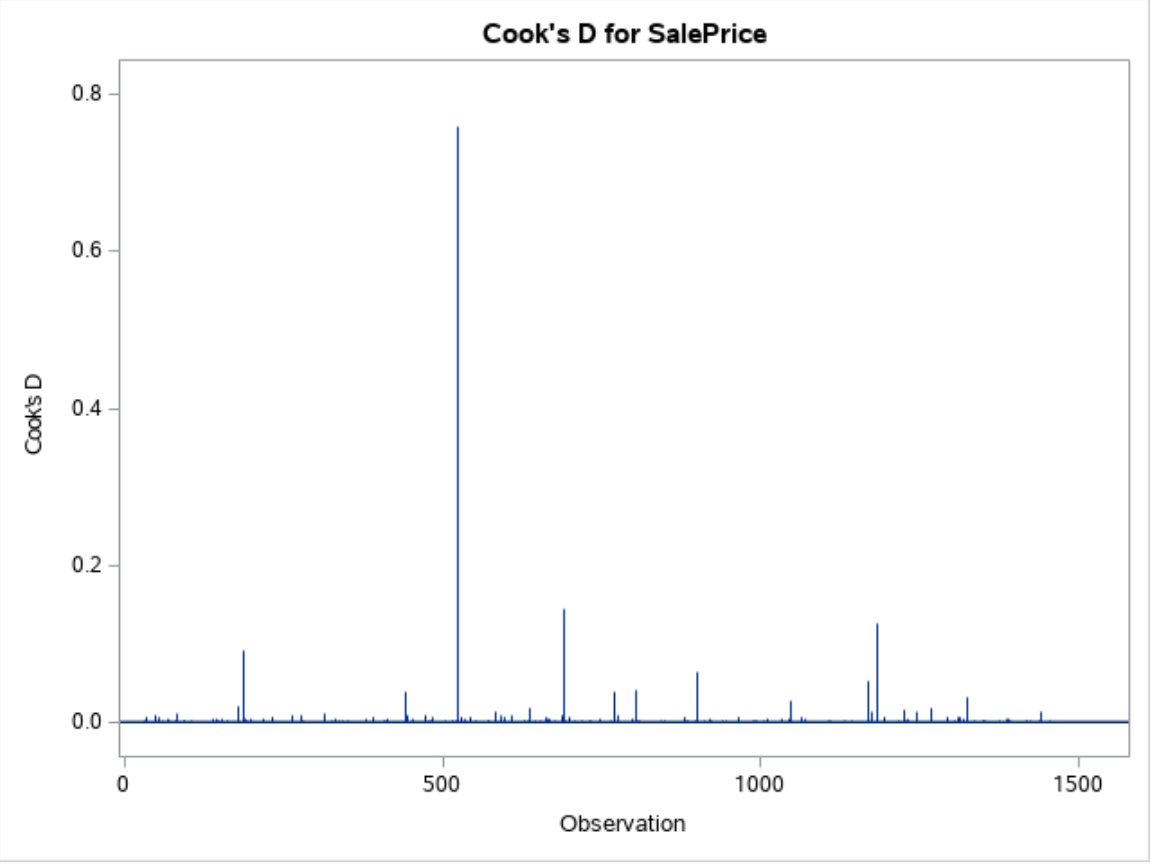
\includegraphics[width=0.48\textwidth]{../graphics/A2FWcooks}} &
		\multicolumn{1}{c|}{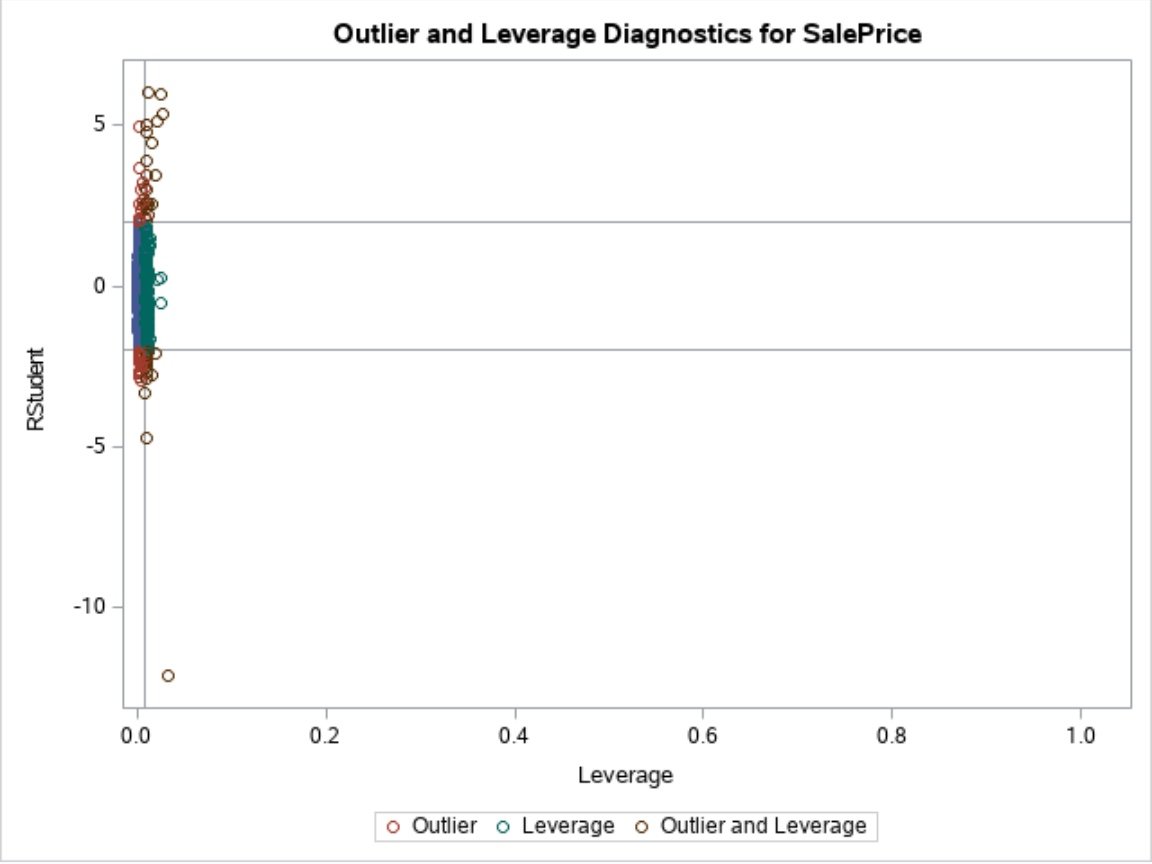
\includegraphics[width=0.48\textwidth]{../graphics/A2FWlev}}\\
		\hline
	\end{tabular}		
	\caption{Influential Point Plots for Forward Selection Model.}
	\label{fig:A2FWIP}
\end{figure}
\begin{figure}[H] % [h] forces the figure to be output where it is defined in the code (it suppresses floating)
	\centering
	\begin{tabular}{| p{0.60\textwidth}|}
	\hline
	\\
	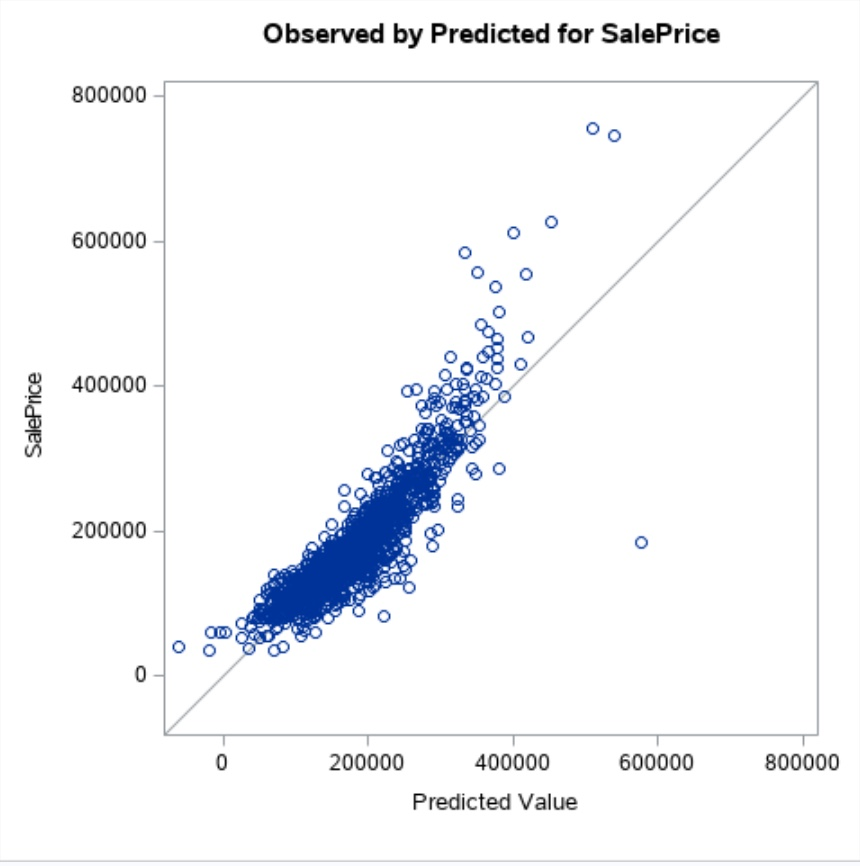
\includegraphics[width=0.60\textwidth]{../graphics/A2BWscatt}\\
	\hline
	\end{tabular}	
	\caption{Scatter Plot Backward Selection Model.}
	\label{fig:A2BWscatt}
\end{figure}
\begin{figure}[H] % [h] forces the figure to be output where it is defined in the code (it suppresses floating)
	\centering
	\begin{tabular}{p{0.48\textwidth} p{0.48\textwidth}}
	\hline
	\multicolumn{1}{|c}{} &  \multicolumn{1}{c|}{} \\
		\multicolumn{1}{|c}{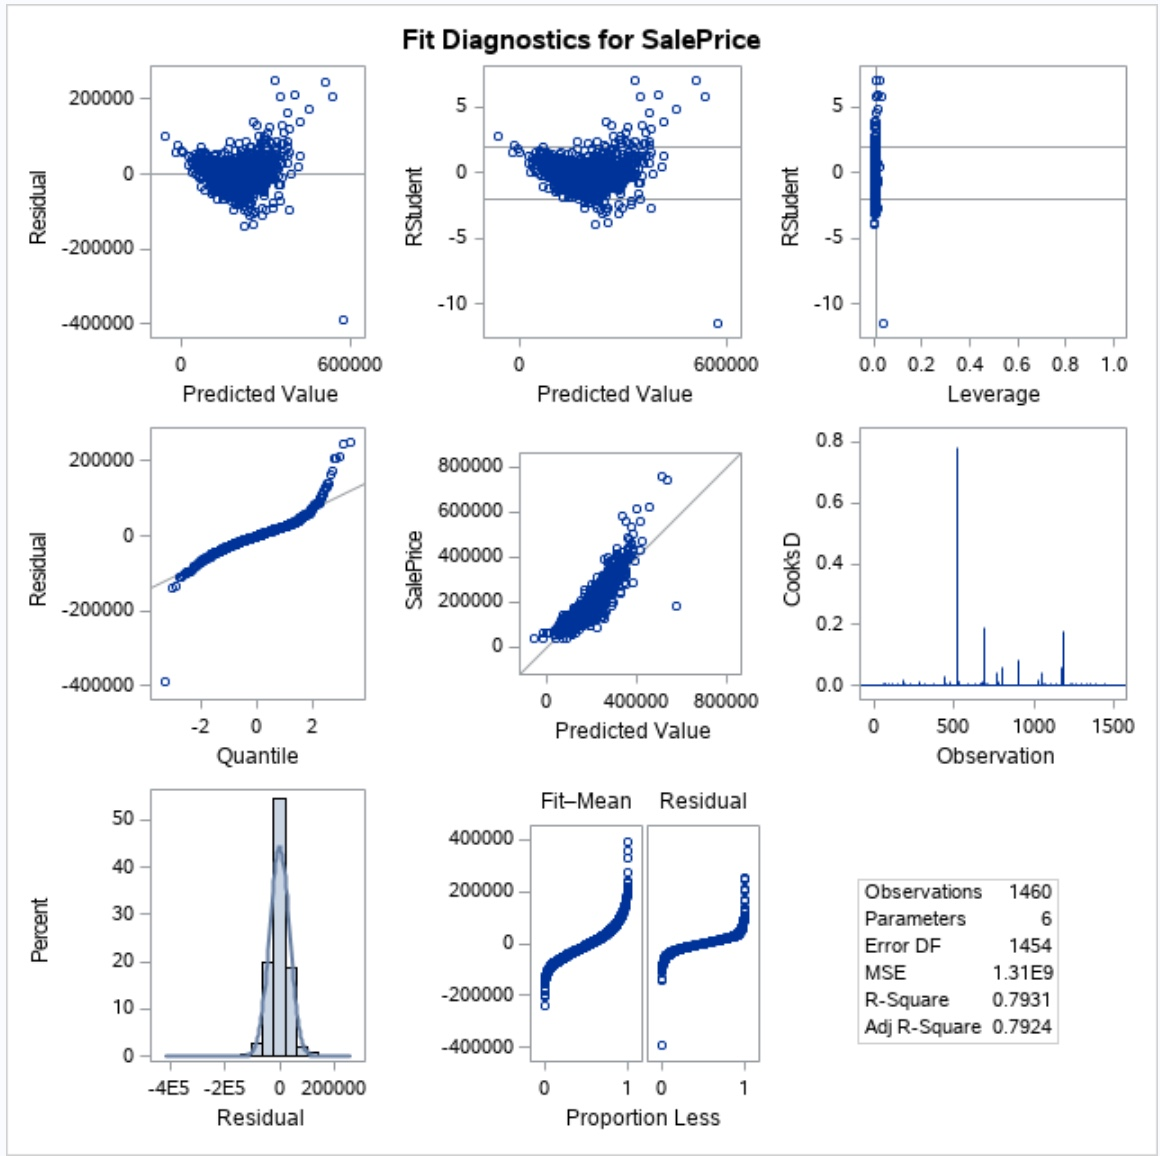
\includegraphics[width=0.48\textwidth]{../graphics/A2BWAss1}} &
		\multicolumn{1}{c|}{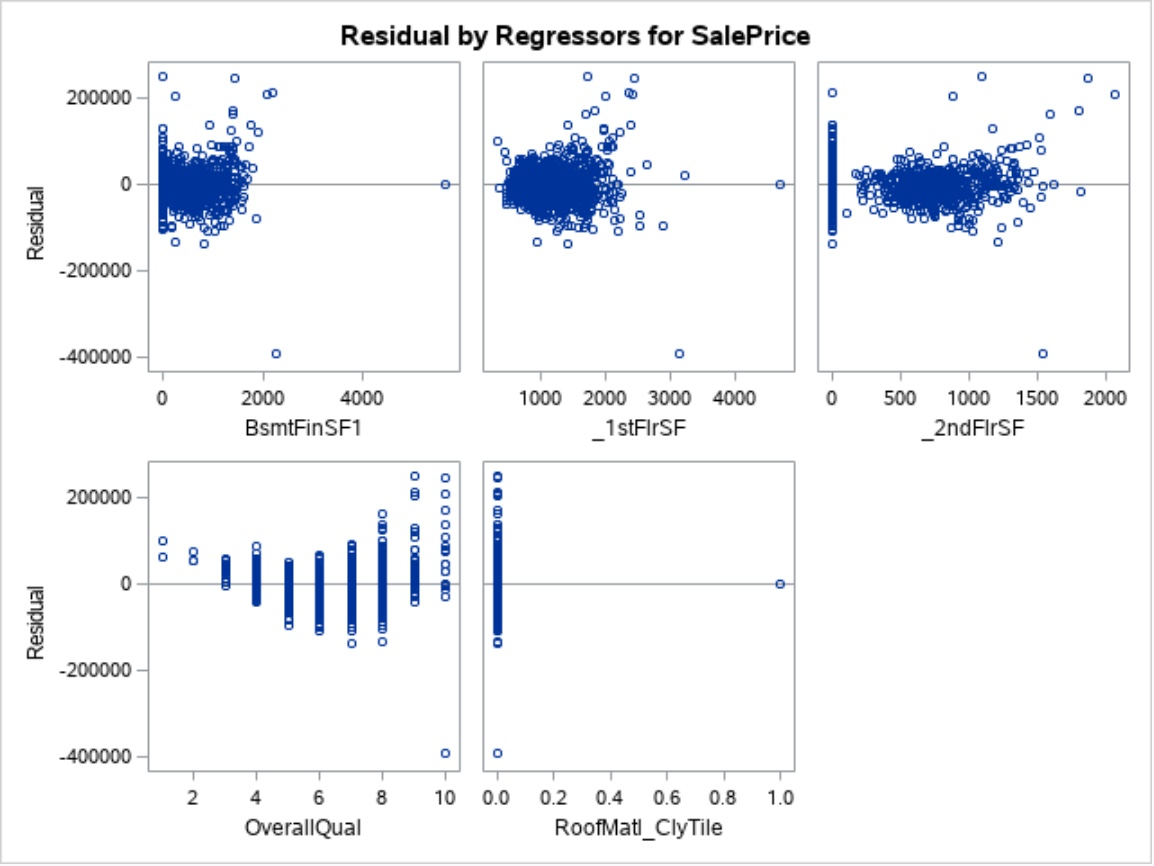
\includegraphics[width=0.48\textwidth]{../graphics/A2BWAss2}}\\
		\hline
	\end{tabular}		
	\caption{Plots for Backward Selection Model.}
	\label{fig:A2BWAss}
\end{figure}
\begin{figure}[H] % [h] forces the figure to be output where it is defined in the code (it suppresses floating)
	\centering
	\begin{tabular}{p{0.48\textwidth} p{0.48\textwidth}}
\hline	
	\multicolumn{1}{|c}{} &  \multicolumn{1}{c|}{} \\
		\multicolumn{1}{|c}{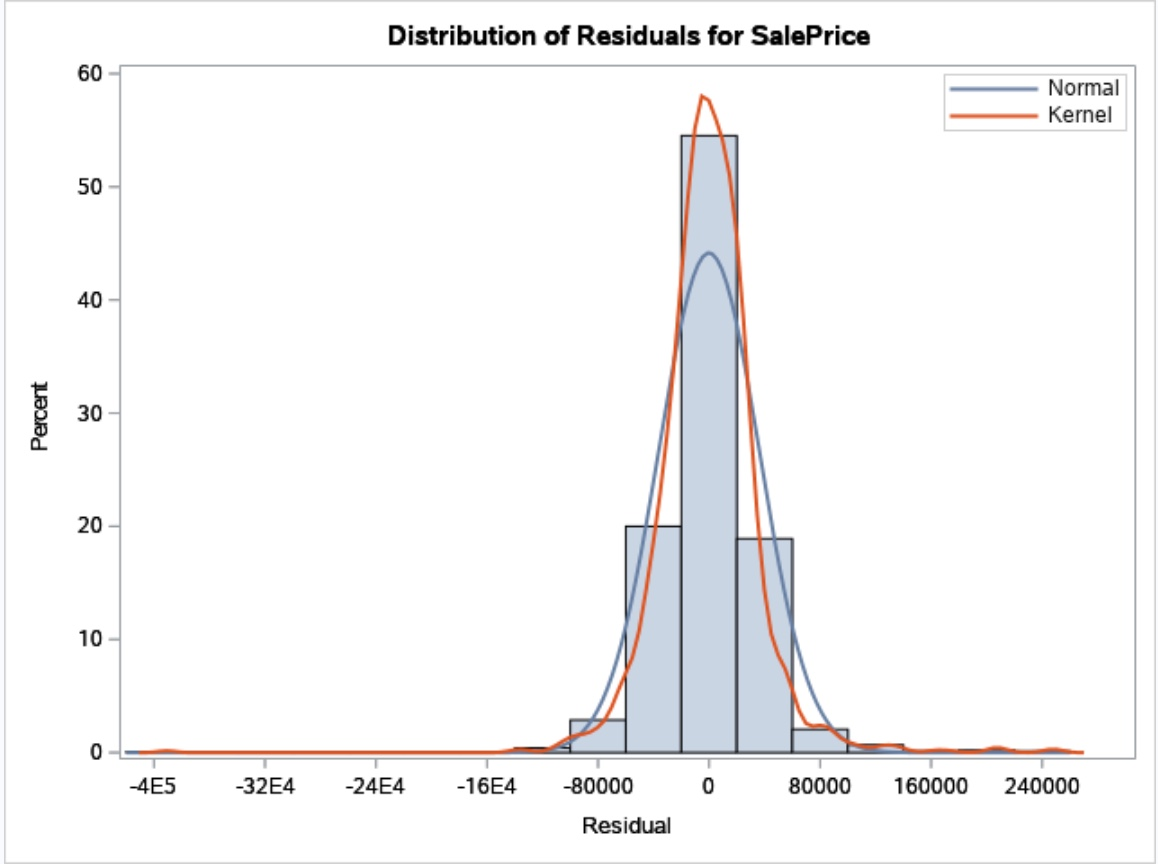
\includegraphics[width=0.48\textwidth]{../graphics/A2BWHist}} &
		\multicolumn{1}{c|}{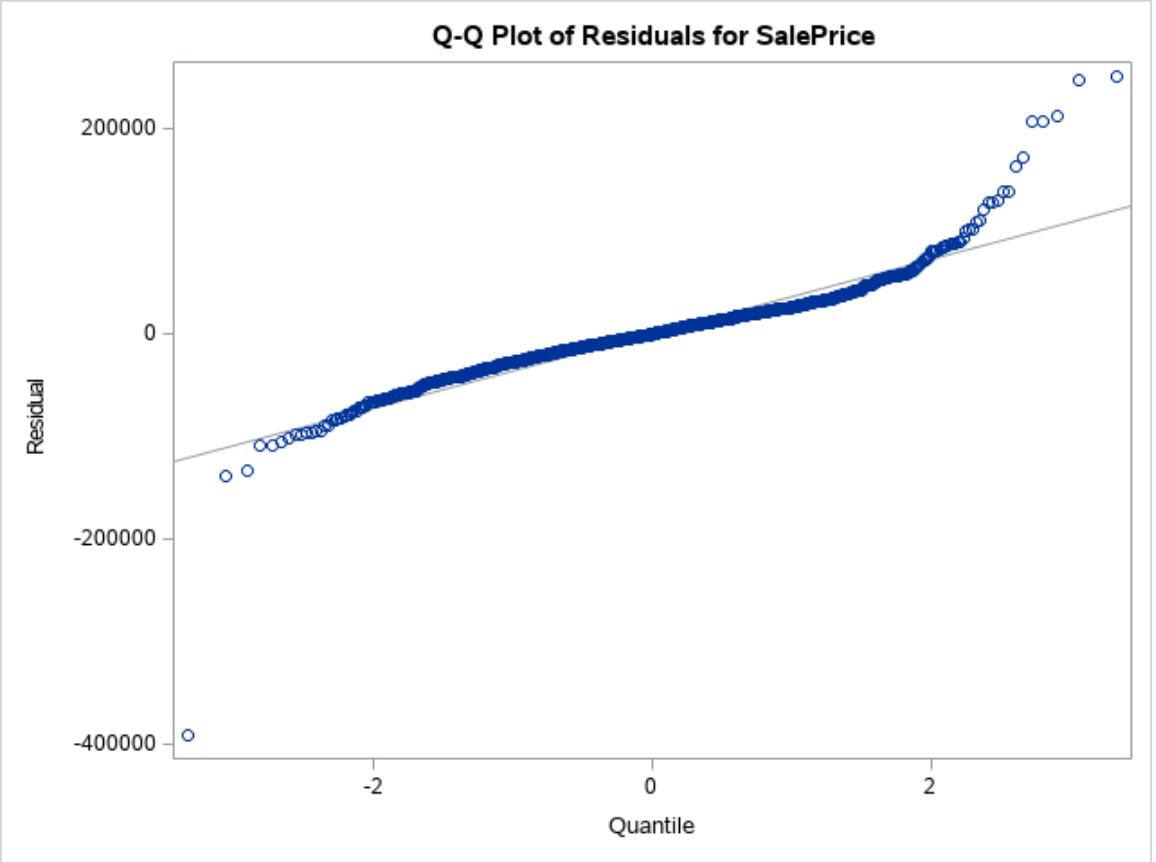
\includegraphics[width=0.48\textwidth]{../graphics/A2BWqq}}\\
		\hline
	\end{tabular}		
	\caption{Normality Plots for Backward Selection Model.}
	\label{fig:A2BWQQ}
\end{figure}
\begin{figure}[H] % [h] forces the figure to be output where it is defined in the code (it suppresses floating)
	\centering
	\begin{tabular}{p{0.48\textwidth} p{0.48\textwidth}}
\hline	
	\multicolumn{1}{|c}{} &  \multicolumn{1}{c|}{} \\
		\multicolumn{1}{|c}{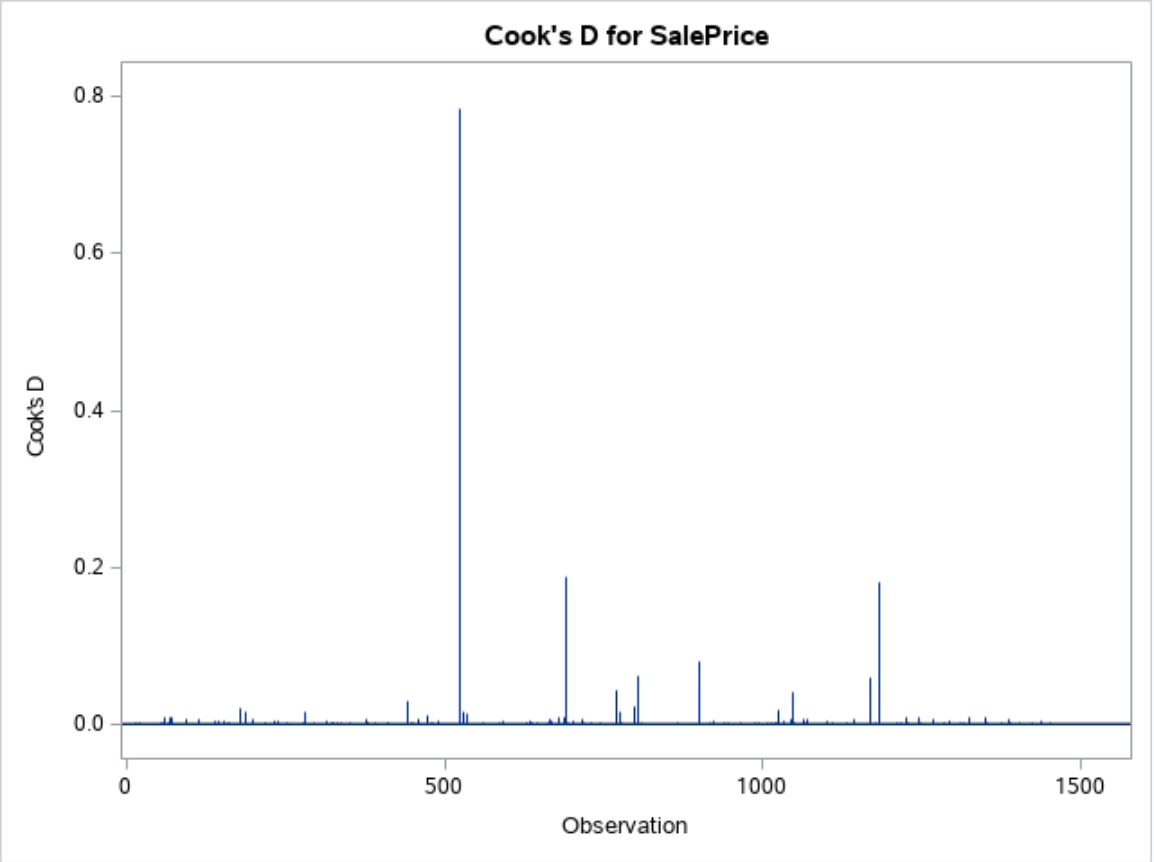
\includegraphics[width=0.48\textwidth]{../graphics/A2BWcooks}} &
		\multicolumn{1}{c|}{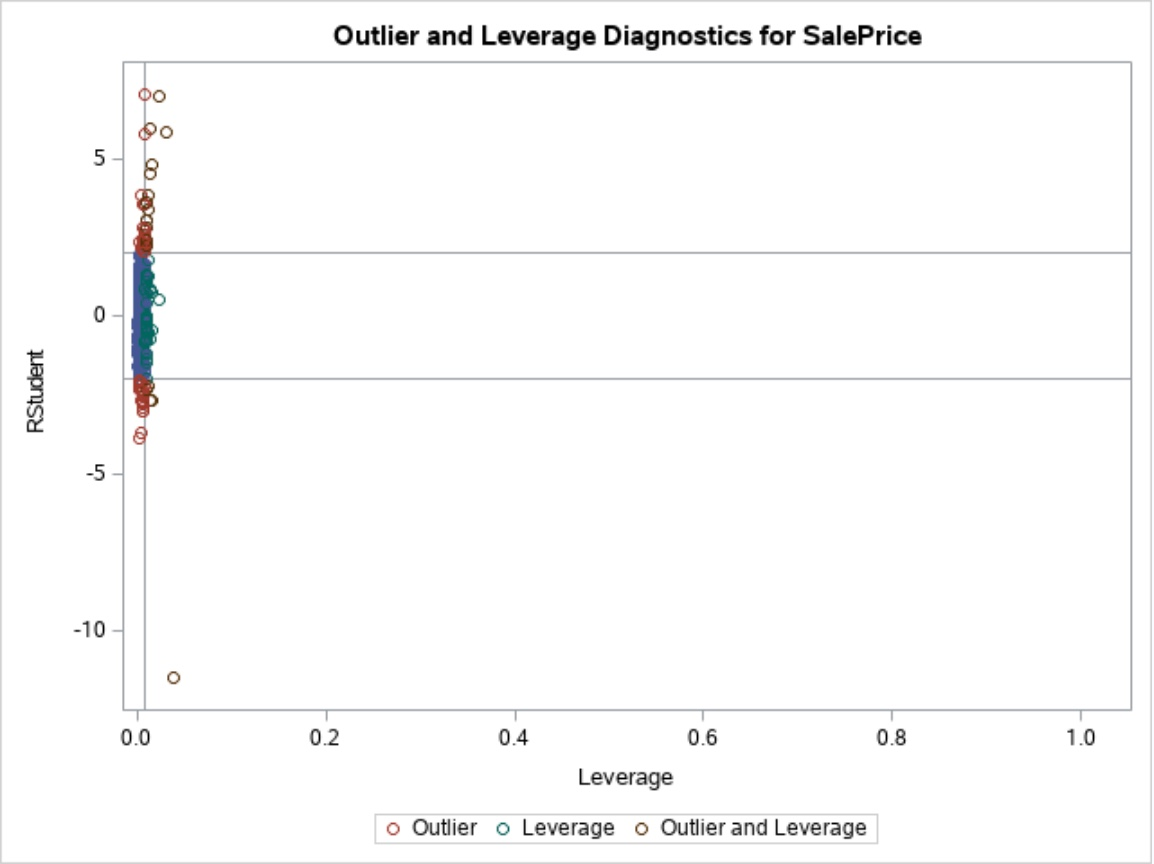
\includegraphics[width=0.48\textwidth]{../graphics/A2BWlev}}\\
		\hline
	\end{tabular}		
	\caption{Influential Point Plots for Backward Selection Model.}
	\label{fig:A2BWIP}
\end{figure}



\begin{figure}[H] % [h] forces the figure to be output where it is defined in the code (it suppresses floating)
	\centering
	\begin{tabular}{| p{0.60\textwidth}|}
	\hline
	\\
	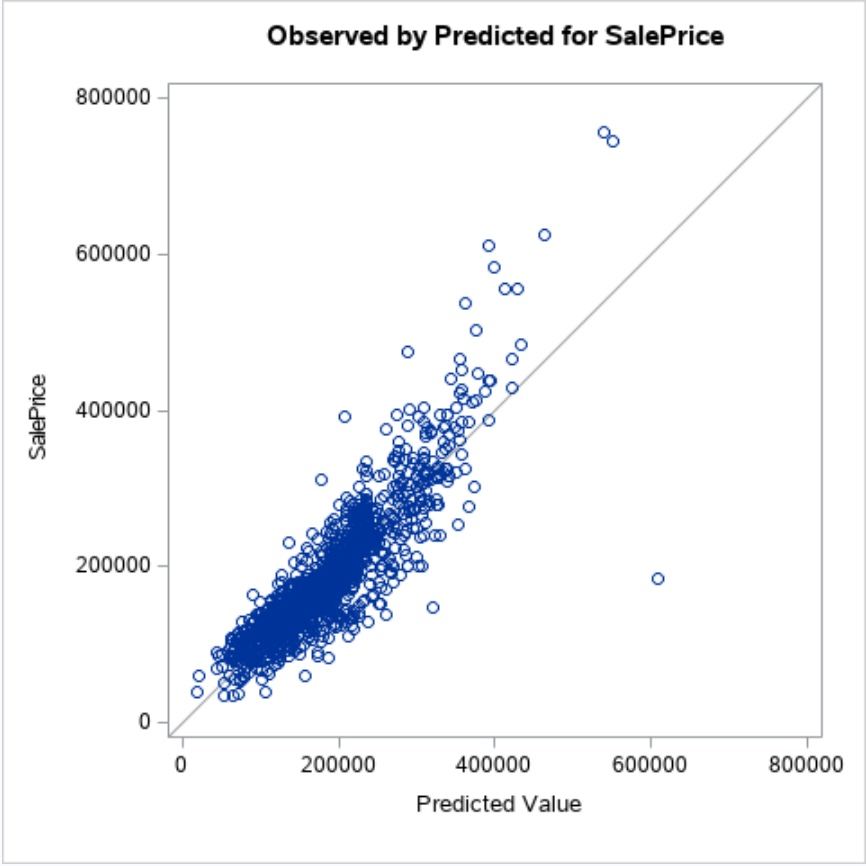
\includegraphics[width=0.60\textwidth]{../graphics/A2SWscatt}\\
	\hline
	\end{tabular}	
	\caption{Scatter Plot Stepwise Selection Model.}
	\label{fig:A2SWscatt}
\end{figure}
\begin{figure}[H] % [h] forces the figure to be output where it is defined in the code (it suppresses floating)
	\centering
	\begin{tabular}{p{0.48\textwidth} p{0.48\textwidth}}
	\hline
	\multicolumn{1}{|c}{} &  \multicolumn{1}{c|}{} \\
		\multicolumn{1}{|c}{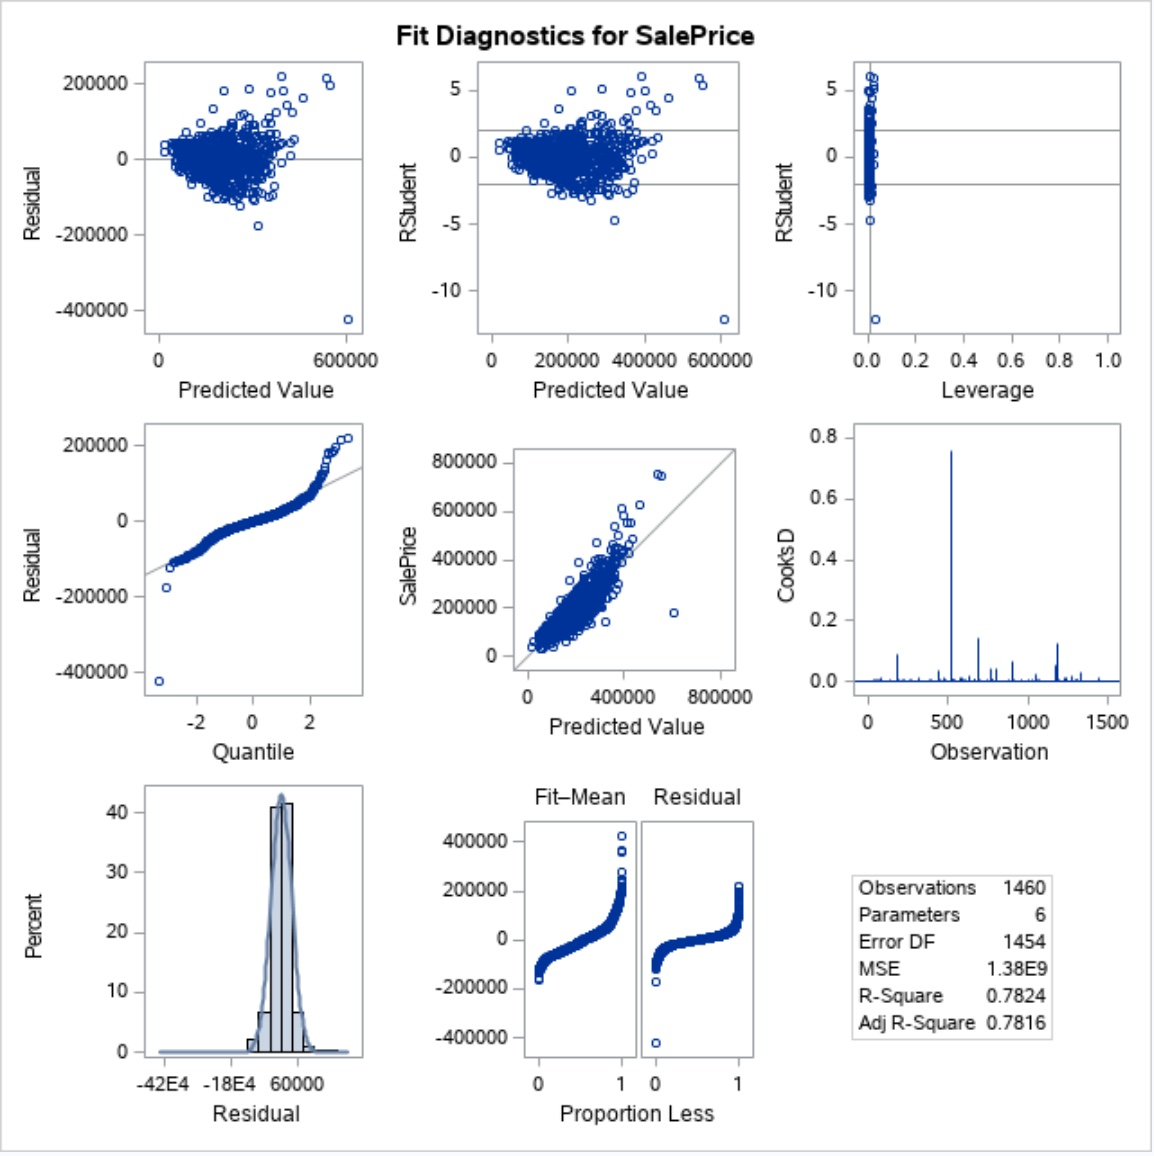
\includegraphics[width=0.48\textwidth]{../graphics/A2SWAss1}} &
		\multicolumn{1}{c|}{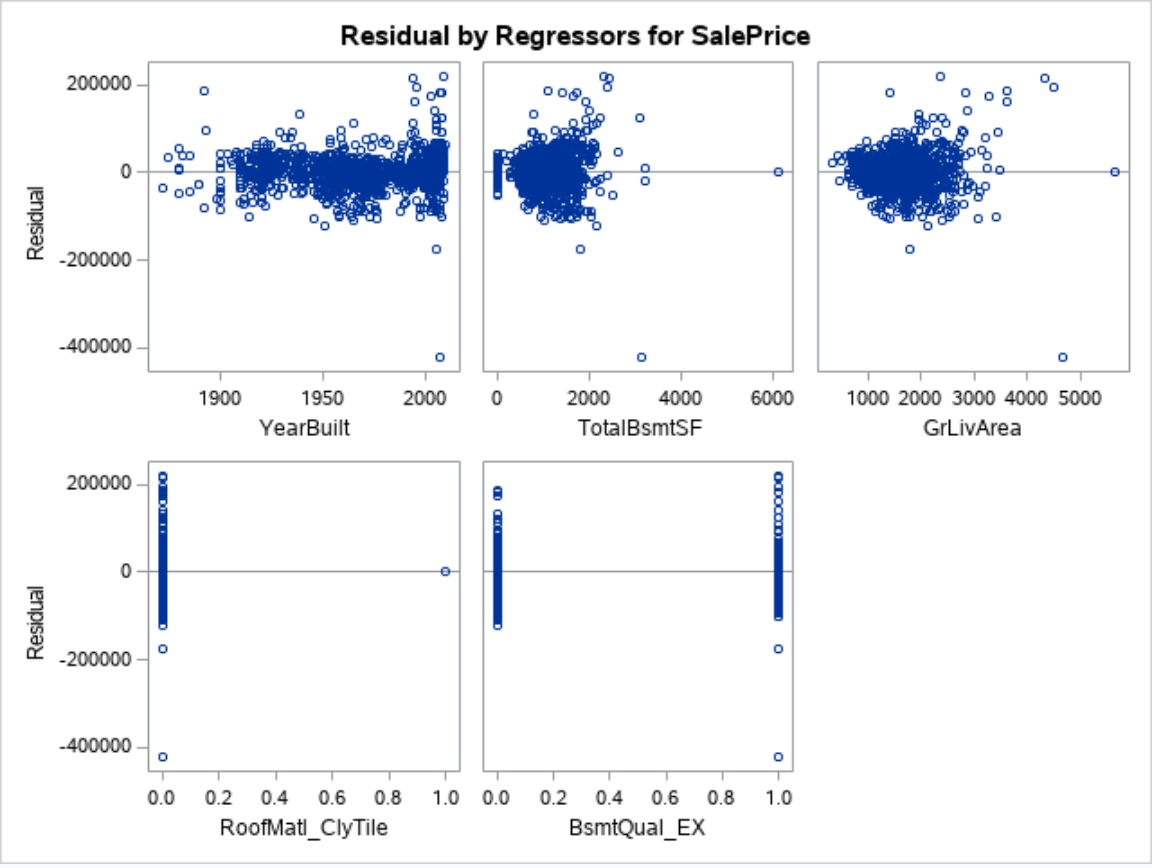
\includegraphics[width=0.48\textwidth]{../graphics/A2SWAss2}}\\
		\hline
	\end{tabular}		
	\caption{Plots for Stepwise Selection Model.}
	\label{fig:A2SWAss}
\end{figure}
\begin{figure}[H] % [h] forces the figure to be output where it is defined in the code (it suppresses floating)
	\centering
	\begin{tabular}{p{0.48\textwidth} p{0.48\textwidth}}
\hline	
	\multicolumn{1}{|c}{} &  \multicolumn{1}{c|}{} \\
		\multicolumn{1}{|c}{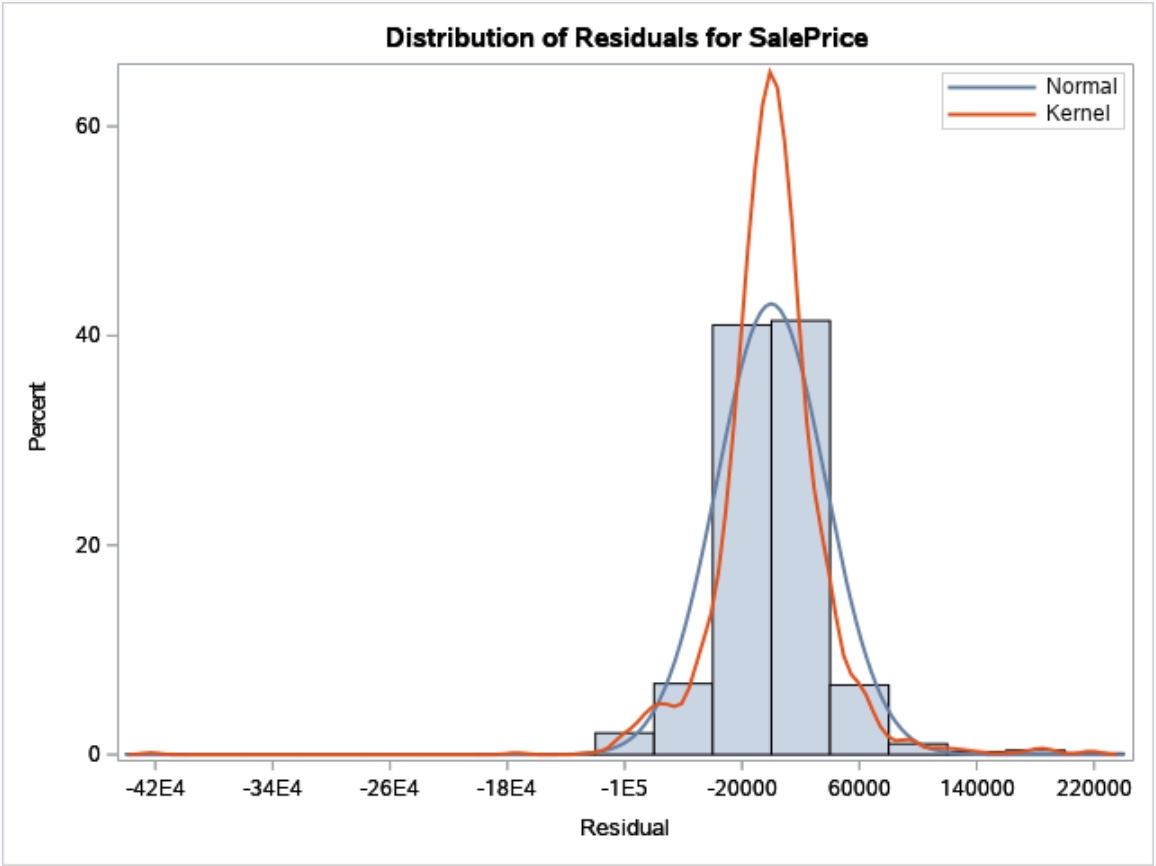
\includegraphics[width=0.48\textwidth]{../graphics/A2SWHist}} &
		\multicolumn{1}{c|}{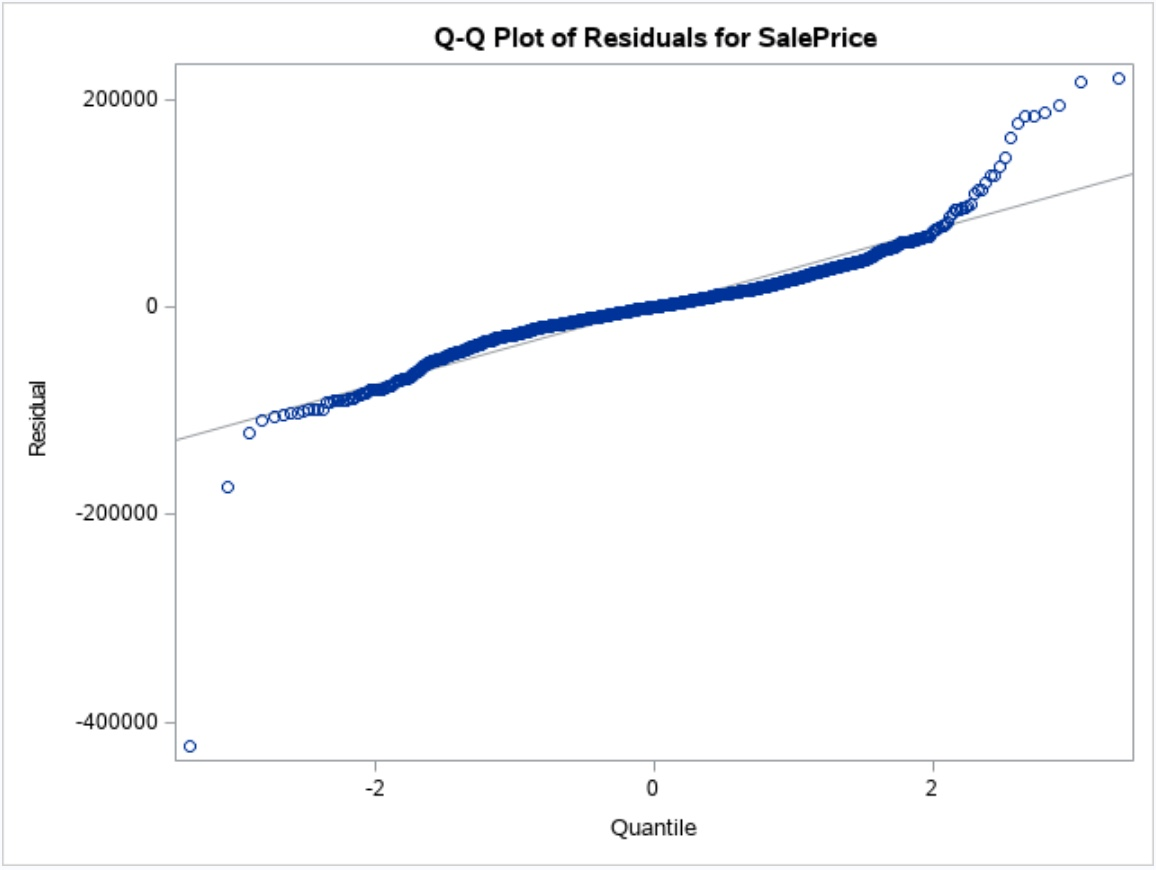
\includegraphics[width=0.48\textwidth]{../graphics/A2SWqq}}\\
		\hline
	\end{tabular}		
	\caption{Normality Plots for Stepwise Selection Model.}
	\label{fig:A2SWQQ}
\end{figure}
\begin{figure}[H] % [h] forces the figure to be output where it is defined in the code (it suppresses floating)
	\centering
	\begin{tabular}{p{0.48\textwidth} p{0.48\textwidth}}
\hline	
	\multicolumn{1}{|c}{} &  \multicolumn{1}{c|}{} \\
		\multicolumn{1}{|c}{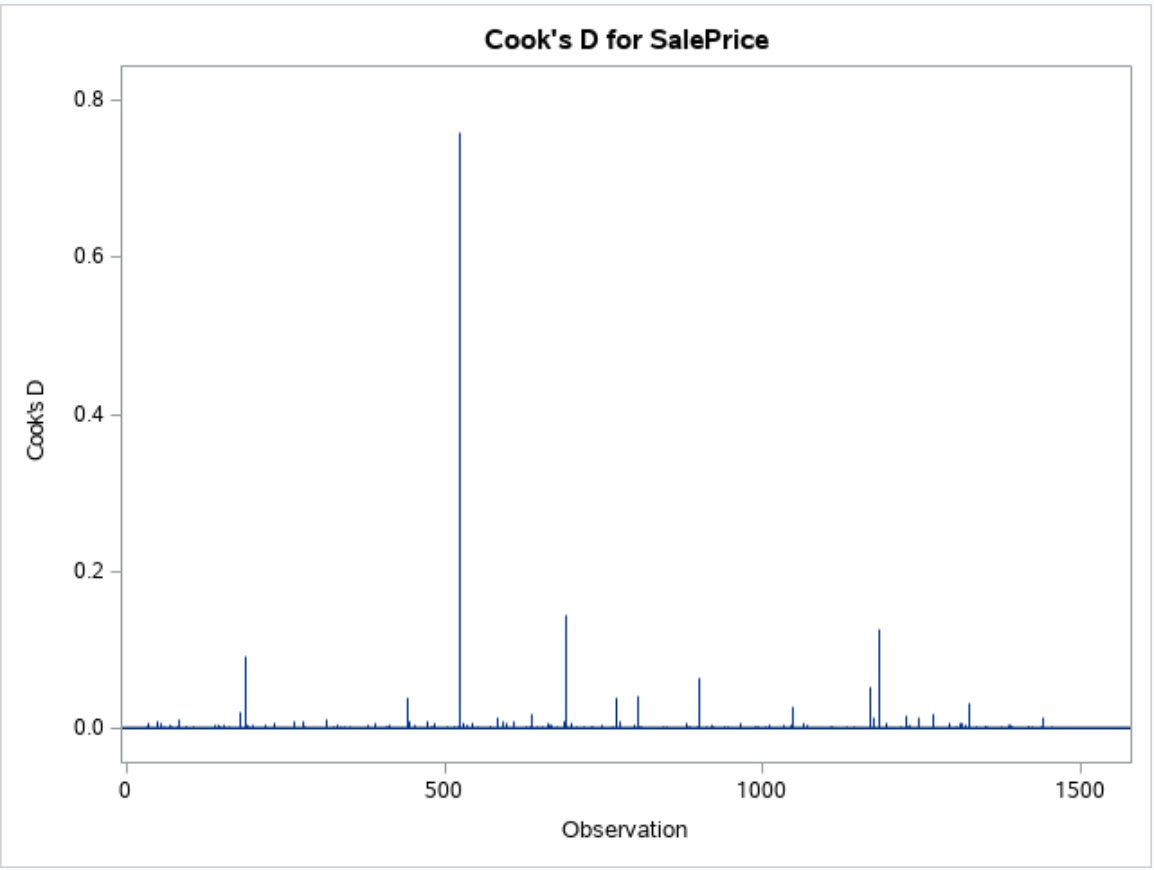
\includegraphics[width=0.48\textwidth]{../graphics/A2SWcooks}} &
		\multicolumn{1}{c|}{\includegraphics[width=0.48\textwidth]{../graphics/A2SWlev}}\\
		\hline
	\end{tabular}		
	\caption{Influential Point Plots for Stepwise Selection Model.}
	\label{fig:A2SWIP}
\end{figure}
\pagebreak

\section{Source Code for Analysis 1}
\label{sec:Analysis1}
\lstinputlisting[
	caption=Analysis 1 SAS Code., % Caption above the listing
	label=lst:Analysis1Source, % Label for referencing this listing
	language=SAS, % Use SAS functions/syntax highlighting
	frame=single, % Frame around the code listing
	showstringspaces=false, % Don't put marks in string spaces
	numbers=left, % Line numbers on left
	numberstyle=\tiny, % Line numbers styling
	]{../code/Analysis1.sas}

%------------------------------------------------

\pagebreak

\section{Source Code for Analysis 2}
\label{sec:Analysis2}

\subsection{Forward Selection}
\lstinputlisting[
	caption=Forward Selection SAS Code., % Caption above the listing
	label=lst:Forward, % Label for referencing this listing
	language=SAS, % Use SAS functions/syntax highlighting
	frame=single, % Frame around the code listing
	showstringspaces=false, % Don't put marks in string spaces
	numbers=left, % Line numbers on left
	numberstyle=\tiny, % Line numbers styling
	]{../code/Forward.sas}

\subsection{Backward Selection}
\lstinputlisting[
	caption=Backward Selection SAS Code., % Caption above the listing
	label=lst:Backward, % Label for referencing this listing
	language=SAS, % Use SAS functions/syntax highlighting
	frame=single, % Frame around the code listing
	showstringspaces=false, % Don't put marks in string spaces
	numbers=left, % Line numbers on left
	numberstyle=\tiny, % Line numbers styling
	]{../code/Backward.sas}

\subsection{Stepwise Selection}
\lstinputlisting[
	caption=Stepwise Selection SAS Code., % Caption above the listing
	label=lst:Stepwise, % Label for referencing this listing
	language=SAS, % Use SAS functions/syntax highlighting
	frame=single, % Frame around the code listing
	showstringspaces=false, % Don't put marks in string spaces
	numbers=left, % Line numbers on left
	numberstyle=\tiny, % Line numbers styling
	]{../code/Stepwise.sas}	

\subsection{Custom Model}
\lstinputlisting[
	caption=Custom Model SAS Code., % Caption above the listing
	label=lst:Custom, % Label for referencing this listing
	language=SAS, % Use SAS functions/syntax highlighting
	frame=single, % Frame around the code listing
	showstringspaces=false, % Don't put marks in string spaces
	numbers=left, % Line numbers on left
	numberstyle=\tiny, % Line numbers styling
	]{../code/Stepwise.sas}	
%------------------------------------------------
\pagebreak

\section{Summary of Data}
\label{sec:DataDescription}
\begin{table}[h] % [h] forces the table to be output where it is defined in the code (it suppresses floating)
	\centering % Centre the table
	\begin{tabular}{|l l l l l|}
		\hline
		\multicolumn{3}{|l|}{Attribute} & \multicolumn{1}{|l|}{} & \multicolumn{1}{|l|}{}\\
		\multicolumn{3}{|l|}{Type} & \multicolumn{1}{|l|}{Description} & \multicolumn{1}{|l|}{Features}\\
		\hline
		& & \multicolumn{1}{|l|}{} & \multicolumn{1}{|l|}{Only provide}& \multicolumn{1}{|l|}{MSSubClass, MSZoning, Street, Alley, LotShape,} \\
		 &  & \multicolumn{1}{|l|}{} & \multicolumn{1}{|l|}{enough information}& \multicolumn{1}{|l|}{LandContour, Utilities, LotConfig, LandSlope,}\\
		& & \multicolumn{1}{|l|}{Nominal} & \multicolumn{1}{|l|}{to distinguish one}& \multicolumn{1}{|l|}{Neighborhood, Condition1, Condition2, BldgType,} \\
& & \multicolumn{1}{|l|}{} & \multicolumn{1}{|l|}{object from another}& \multicolumn{1}{|l|}{HouseStyle, RoofMatl, Exterior1st, Exterior2nd,} \\
		\multirow{2}{*}{\STAB{\rotatebox[origin=c]{90}{Categorical}}}		& \multirow{2}{*}{\STAB{\rotatebox[origin=c]				{90}{(Qualitative)}}}& \multicolumn{1}{|l|}{} & \multicolumn{1}{|l|}{}& \multicolumn{1}{|l|}{MasVnrType, Foundation, BsmtExposure, Heating} \\
				& & \multicolumn{1}{|l|}{} & \multicolumn{1}{|l|}{}& \multicolumn{1}{|l|}{CentralAir, Electrical, GarageType, GarageFinish} \\
				& & \multicolumn{1}{|l|}{} & \multicolumn{1}{|l|}{}& \multicolumn{1}{|l|}{PavedDrive, MiscFeature, SaleType, SaleCondition} \\	
				& & \multicolumn{1}{|l|}{} & \multicolumn{1}{|l|}{}& \multicolumn{1}{|l|}{RoofStyle \textbf{(30 variables)}} \\
			\cline{3-5}
		& & \multicolumn{1}{|l|}{} & \multicolumn{1}{|l|}{Provide enough}& \multicolumn{1}{|l|}{OverallQual, OverallCond, ExterQual, ExterCond,} \\
		& & \multicolumn{1}{|l|}{Ordinal} & \multicolumn{1}{|l|}{information to}& \multicolumn{1}{|l|}{BsmtQual, BsmtCond, BsmtFinType1,} \\
				& & \multicolumn{1}{|l|}{} & \multicolumn{1}{|l|}{order objects}& \multicolumn{1}{|l|}{BsmtFinType2, HeatingQC, KitchenQual, Functional,} \\
				& & \multicolumn{1}{|l|}{} & \multicolumn{1}{|l|}{}& \multicolumn{1}{|l|}{FireplaceQu, GarageQual, GarageCond, PoolQC,} \\					& & \multicolumn{1}{|l|}{} & \multicolumn{1}{|l|}{}& \multicolumn{1}{|l|}{Fence \textbf{(16 variables)}} \\				
\hline
		& & \multicolumn{1}{|l|}{} & \multicolumn{1}{|l|}{Interval attributes}& \multicolumn{1}{|l|}{YearBuilt, YearRemodAdd, GarageYrBlt, MoSold,} \\
		 &  & \multicolumn{1}{|l|}{Interval} & \multicolumn{1}{|l|}{difference between}& \multicolumn{1}{|l|}{YrSold \textbf{(5 variables)}}\\
		& & \multicolumn{1}{|l|}{} & \multicolumn{1}{|l|}{values are}& \multicolumn{1}{|l|}{} \\
	& \multirow{2}{*}{\STAB{\rotatebox[origin=c]				{90}{(Quantitative)}}}& \multicolumn{1}{|l|}{} & \multicolumn{1}{|l|}{meaningful}& \multicolumn{1}{|l|}{} \\
		\cline{3-5}
\multirow{2}{*}{\STAB{\rotatebox[origin=c]{90}{Numeric}}}			& & \multicolumn{1}{|l|}{} & \multicolumn{1}{|l|}{Differences and}& \multicolumn{1}{|l|}{LotFrontage, LotArea, BsmtFinSF1, BsmtFinSF2,} \\
		& & \multicolumn{1}{|l|}{Ratio} & \multicolumn{1}{|l|}{ratios are}& \multicolumn{1}{|l|}{BsmtUnfSF, TotalBsmtSF, 1stFlrSF, 2ndFlrSF,} \\
				& & \multicolumn{1}{|l|}{} & \multicolumn{1}{|l|}{meaningful}& \multicolumn{1}{|l|}{LowQualFinSF, GrLivArea, BsmtFullBath,} \\
								& & \multicolumn{1}{|l|}{} & \multicolumn{1}{|l|}{}& \multicolumn{1}{|l|}{MasVnrArea, BsmtHalfBath, FullBath, HalfBath,} \\
& & \multicolumn{1}{|l|}{} & \multicolumn{1}{|l|}{}& \multicolumn{1}{|l|}{Bedroom, Kitchen, TotRmsAbvGrd, Fireplaces,} \\
& & \multicolumn{1}{|l|}{} & \multicolumn{1}{|l|}{}& \multicolumn{1}{|l|}{GarageCars, GarageArea, WoodDeckSF, OpenPorchSF,} \\
& & \multicolumn{1}{|l|}{} & \multicolumn{1}{|l|}{}& \multicolumn{1}{|l|}{EnclosedPorch, 3SsnPorch, ScreenPorch, PoolArea,} \\
& & \multicolumn{1}{|l|}{} & \multicolumn{1}{|l|}{}& \multicolumn{1}{|l|}{MiscVal \textbf{(28 variables)}} \\
\hline

	\end{tabular}
	\caption{Summary of Dataset}
	\label{tab:Data}
\end{table}

\begin{center}
\begin{tabular}{c c c c c c}
\hline
\multicolumn{6}{|c|}{Classification Variables}\\
\hline
\multicolumn{2}{|c}{MSSubClass} & \multicolumn{4}{l|}{Identifies the type of dwelling involved in the sale}\\ 
\multicolumn{2}{|c}{} & \multicolumn{1}{c}{20} & \multicolumn{3}{l|}{1-STORY 1946 \& NEWER ALL STYLES}\\
\multicolumn{2}{|c}{} & \multicolumn{1}{c}{30} & \multicolumn{3}{l|}{1-STORY 1945 \& OLDER}\\
\multicolumn{2}{|c}{} & \multicolumn{1}{c}{40} & \multicolumn{3}{l|}{1-STORY W/FINISHED ATTIC ALL AGES}\\
\multicolumn{2}{|c}{} & \multicolumn{1}{c}{45} & \multicolumn{3}{l|}{1-1/2 STORY - UNFINISHED ALL AGES}\\
\multicolumn{2}{|c}{} & \multicolumn{1}{c}{50} & \multicolumn{3}{l|}{1-1/2 STORY FINISHED ALL AGES}\\
\multicolumn{2}{|c}{} & \multicolumn{1}{c}{60} & \multicolumn{3}{l|}{2-STORY 1946 \& NEWER}\\
\multicolumn{2}{|c}{} & \multicolumn{1}{c}{70} & \multicolumn{3}{l|}{2-STORY 1945 \& OLDER}\\
\multicolumn{2}{|c}{} & \multicolumn{1}{c}{75} & \multicolumn{3}{l|}{2-1/2 STORY ALL AGES}\\
\multicolumn{2}{|c}{} & \multicolumn{1}{c}{80} & \multicolumn{3}{l|}{SPLIT OR MULTI-LEVEL}\\
\multicolumn{2}{|c}{} & \multicolumn{1}{c}{85} & \multicolumn{3}{l|}{SPLIT FOYER}\\
\multicolumn{2}{|c}{} & \multicolumn{1}{c}{90} & \multicolumn{3}{l|}{DUPLEX - ALL STYLES AND AGES}\\
\multicolumn{2}{|c}{} & \multicolumn{1}{c}{120} & \multicolumn{3}{l|}{1-STORY PUD (Planned Unit Development) - 1946 \& NEWER}\\
\multicolumn{2}{|c}{} & \multicolumn{1}{c}{150} & \multicolumn{3}{l|}{1-1/2 STORY PUD - ALL AGES}\\
\multicolumn{2}{|c}{} & \multicolumn{1}{c}{160} & \multicolumn{3}{l|}{2-STORY PUD - 1946 \& NEWER}\\
\multicolumn{2}{|c}{} & \multicolumn{1}{c}{180} & \multicolumn{3}{l|}{PUD - MULTILEVEL - INCL SPLIT LEV/FOYER}\\
\multicolumn{2}{|c}{} & \multicolumn{1}{c}{190} & \multicolumn{3}{l|}{2 FAMILY CONVERSION - ALL STYLES AND AGES}\\
\hline
\multicolumn{2}{|c}{MSZoning} & \multicolumn{4}{l|}{Identifies the general zoning classification of the sale}\\ 
\multicolumn{2}{|c}{} & \multicolumn{1}{c}{A} & \multicolumn{3}{l|}{Agriculture}\\
\multicolumn{2}{|c}{} & \multicolumn{1}{c}{C} & \multicolumn{3}{l|}{Commercial}\\
\multicolumn{2}{|c}{} & \multicolumn{1}{c}{FV} & \multicolumn{3}{l|}{Floating Village Residential}\\
\multicolumn{2}{|c}{} & \multicolumn{1}{c}{I} & \multicolumn{3}{l|}{Industrial}\\
\multicolumn{2}{|c}{} & \multicolumn{1}{c}{RH} & \multicolumn{3}{l|}{Residential High Density}\\
\multicolumn{2}{|c}{} & \multicolumn{1}{c}{RL} & \multicolumn{3}{l|}{Residential Low Density}\\
\multicolumn{2}{|c}{} & \multicolumn{1}{c}{RP} & \multicolumn{3}{l|}{Residential Low Density Park}\\
\multicolumn{2}{|c}{} & \multicolumn{1}{c}{RM} & \multicolumn{3}{l|}{Residential Medium Density}\\
\hline	
\multicolumn{2}{|c}{LotFrontage} & \multicolumn{4}{l|}{Linear feet of street connected to property}\\
\hline
\multicolumn{2}{|c}{LotArea} & \multicolumn{4}{l|}{Lot size in square feet}\\
\hline
\multicolumn{2}{|c}{Street} & \multicolumn{4}{l|}{Type of road access to property}\\ 
\multicolumn{2}{|c}{} & \multicolumn{1}{c}{Grvl} & \multicolumn{3}{l|}{Gravel}\\
\multicolumn{2}{|c}{} & \multicolumn{1}{c}{Pave} & \multicolumn{3}{l|}{Paved}\\
\hline
\multicolumn{2}{|c}{Alley} & \multicolumn{4}{l|}{Type of alley access to property}\\ 
\multicolumn{2}{|c}{} & \multicolumn{1}{c}{Grvl} & \multicolumn{3}{l|}{Gravel}\\
\multicolumn{2}{|c}{} & \multicolumn{1}{c}{Pave} & \multicolumn{3}{l|}{Paved}\\
\multicolumn{2}{|c}{} & \multicolumn{1}{c}{NA} & \multicolumn{3}{l|}{No alley access}\\
\hline
\multicolumn{2}{|c}{LotShape} & \multicolumn{4}{l|}{General shape of property}\\ 
\multicolumn{2}{|c}{} & \multicolumn{1}{c}{Reg} & \multicolumn{3}{l|}{Regular}\\
\multicolumn{2}{|c}{} & \multicolumn{1}{c}{IR1} & \multicolumn{3}{l|}{Slightly Irregular}\\
\multicolumn{2}{|c}{} & \multicolumn{1}{c}{IR2} & \multicolumn{3}{l|}{Moderately Irregular}\\
\multicolumn{2}{|c}{} & \multicolumn{1}{c}{IR3} & \multicolumn{3}{l|}{Irregular}\\
\hline
\multicolumn{2}{|c}{LandContour} & \multicolumn{4}{l|}{General shape of property}\\ 
\multicolumn{2}{|c}{} & \multicolumn{1}{c}{Lvl} & \multicolumn{3}{l|}{Near Flat/Level}\\
\multicolumn{2}{|c}{} & \multicolumn{1}{c}{Bnk} & \multicolumn{3}{l|}{Banked - Quick and significant rise from street grade to building}\\
\multicolumn{2}{|c}{} & \multicolumn{1}{c}{HLS} & \multicolumn{3}{l|}{Hillside - Significant slope from side to side}\\
\multicolumn{2}{|c}{} & \multicolumn{1}{c}{Low} & \multicolumn{3}{l|}{Depression}\\
\hline
\end{tabular}
\end{center}
\begin{center}
\begin{tabular}{c c c c c c}
\hline
\multicolumn{6}{|c|}{Classification Variables}\\
\hline
\multicolumn{2}{|c}{Utilities} & \multicolumn{4}{l|}{Identifies the type of dwelling involved in the sale}\\ 
\multicolumn{2}{|c}{} & \multicolumn{1}{c}{AllPub} & \multicolumn{3}{l|}{All public Utilities (E,G,W,\& S)	}\\
\multicolumn{2}{|c}{} & \multicolumn{1}{c}{NoSewr} & \multicolumn{3}{l|}{Electricity, Gas, and Water (Septic Tank)}\\
\multicolumn{2}{|c}{} & \multicolumn{1}{c}{NoSeWa} & \multicolumn{3}{l|}{Electricity and Gas Only}\\
\multicolumn{2}{|c}{} & \multicolumn{1}{c}{ELO} & \multicolumn{3}{l|}{Electricity only}\\
\hline
\multicolumn{2}{|c}{LotConfig} & \multicolumn{4}{l|}{Lot configuration}\\ 
\multicolumn{2}{|c}{} & \multicolumn{1}{c}{Inside} & \multicolumn{3}{l|}{Inside lot}\\
\multicolumn{2}{|c}{} & \multicolumn{1}{c}{Corner} & \multicolumn{3}{l|}{Corner lot}\\
\multicolumn{2}{|c}{} & \multicolumn{1}{c}{CulDSac} & \multicolumn{3}{l|}{Cul-de-sac}\\
\multicolumn{2}{|c}{} & \multicolumn{1}{c}{FR2} & \multicolumn{3}{l|}{Frontage on 2 sides of property}\\
\multicolumn{2}{|c}{} & \multicolumn{1}{c}{FR3} & \multicolumn{3}{l|}{Frontage on 3 sides of property}\\
\hline
\multicolumn{2}{|c}{LandSlope} & \multicolumn{4}{l|}{Slope of property}\\ 
\multicolumn{2}{|c}{} & \multicolumn{1}{c}{Gtl} & \multicolumn{3}{l|}{Gentle slope}\\
\multicolumn{2}{|c}{} & \multicolumn{1}{c}{Mod} & \multicolumn{3}{l|}{Moderate slope}\\
\multicolumn{2}{|c}{} & \multicolumn{1}{c}{Sev} & \multicolumn{3}{l|}{Severe slope}\\
\hline
\multicolumn{2}{|c}{Neighborhood} & \multicolumn{4}{l|}{Physical locations within Ames city limits}\\ 
\multicolumn{2}{|c}{} & \multicolumn{1}{c}{Blmgtn} & \multicolumn{3}{l|}{Bloomington Heights}\\
\multicolumn{2}{|c}{} & \multicolumn{1}{c}{Blueste} & \multicolumn{3}{l|}{Bluestem}\\
\multicolumn{2}{|c}{} & \multicolumn{1}{c}{BrDale} & \multicolumn{3}{l|}{Briardale}\\
\multicolumn{2}{|c}{} & \multicolumn{1}{c}{BrkSide} & \multicolumn{3}{l|}{Brookside}\\
\multicolumn{2}{|c}{} & \multicolumn{1}{c}{ClearCr} & \multicolumn{3}{l|}{Clear Creek}\\
\multicolumn{2}{|c}{} & \multicolumn{1}{c}{CollgCr} & \multicolumn{3}{l|}{College Creek}\\
\multicolumn{2}{|c}{} & \multicolumn{1}{c}{Crawfor} & \multicolumn{3}{l|}{Crawford}\\
\multicolumn{2}{|c}{} & \multicolumn{1}{c}{Edwards} & \multicolumn{3}{l|}{Edwards}\\
\multicolumn{2}{|c}{} & \multicolumn{1}{c}{Gilbert} & \multicolumn{3}{l|}{Gilbert}\\
\multicolumn{2}{|c}{} & \multicolumn{1}{c}{IDOTRR} & \multicolumn{3}{l|}{Iowa DOT and Rail Road}\\
\multicolumn{2}{|c}{} & \multicolumn{1}{c}{MeadowV} & \multicolumn{3}{l|}{Meadow Village}\\
\multicolumn{2}{|c}{} & \multicolumn{1}{c}{Mitchel} & \multicolumn{3}{l|}{Mitchell}\\
\multicolumn{2}{|c}{} & \multicolumn{1}{c}{NAmes} & \multicolumn{3}{l|}{North Ames}\\
\multicolumn{2}{|c}{} & \multicolumn{1}{c}{NoRidge} & \multicolumn{3}{l|}{Northridge}\\
\multicolumn{2}{|c}{} & \multicolumn{1}{c}{NPkVill} & \multicolumn{3}{l|}{Northpark Villa}\\
\multicolumn{2}{|c}{} & \multicolumn{1}{c}{NridgHt} & \multicolumn{3}{l|}{Northridge Heights}\\
\multicolumn{2}{|c}{} & \multicolumn{1}{c}{NWAmes} & \multicolumn{3}{l|}{Northwest Ames}\\
\multicolumn{2}{|c}{} & \multicolumn{1}{c}{OldTown} & \multicolumn{3}{l|}{Old Town}\\
\multicolumn{2}{|c}{} & \multicolumn{1}{c}{SWISU} & \multicolumn{3}{l|}{South \& West of Iowa State University}\\
\multicolumn{2}{|c}{} & \multicolumn{1}{c}{Sawyer} & \multicolumn{3}{l|}{Sawyer}\\
\multicolumn{2}{|c}{} & \multicolumn{1}{c}{SawyerW} & \multicolumn{3}{l|}{Sawyer West}\\
\multicolumn{2}{|c}{} & \multicolumn{1}{c}{Somerst} & \multicolumn{3}{l|}{Somerset}\\
\multicolumn{2}{|c}{} & \multicolumn{1}{c}{StoneBr} & \multicolumn{3}{l|}{Stone Brook}\\
\multicolumn{2}{|c}{} & \multicolumn{1}{c}{Timber} & \multicolumn{3}{l|}{Timberland}\\
\multicolumn{2}{|c}{} & \multicolumn{1}{c}{Veenker} & \multicolumn{3}{l|}{Veenker}\\
\hline
\multicolumn{2}{|c}{Condition1} & \multicolumn{4}{l|}{Proximity to various conditions}\\ 
\multicolumn{2}{|c}{} & \multicolumn{1}{c}{Artery} & \multicolumn{3}{l|}{Adjacent to arterial street}\\
\multicolumn{2}{|c}{} & \multicolumn{1}{c}{Feedr} & \multicolumn{3}{l|}{Adjacent to feeder street}\\
\multicolumn{2}{|c}{} & \multicolumn{1}{c}{Norm} & \multicolumn{3}{l|}{Normal}\\
\multicolumn{2}{|c}{} & \multicolumn{1}{c}{RRNn} & \multicolumn{3}{l|}{Within 200' of North-South Railroad}\\
\multicolumn{2}{|c}{} & \multicolumn{1}{c}{RRAn} & \multicolumn{3}{l|}{Adjacent to North-South Railroad}\\
\multicolumn{2}{|c}{} & \multicolumn{1}{c}{PosN} & \multicolumn{3}{l|}{Near positive off-site feature--park, greenbelt, etc.}\\
\multicolumn{2}{|c}{} & \multicolumn{1}{c}{PosA} & \multicolumn{3}{l|}{Adjacent to postive off-site feature}\\
\multicolumn{2}{|c}{} & \multicolumn{1}{c}{RRNe} & \multicolumn{3}{l|}{Within 200' of East-West Railroad}\\
\multicolumn{2}{|c}{} & \multicolumn{1}{c}{RRAe} & \multicolumn{3}{l|}{Adjacent to East-West Railroad}\\
\hline
\end{tabular}
\end{center}
\begin{center}
\begin{tabular}{c c c c c c}
\hline
\multicolumn{6}{|c|}{Classification Variables}\\
\hline
\multicolumn{2}{|c}{Condition2} & \multicolumn{4}{l|}{Proximity to various conditions (if more than one is present)}\\ 
\multicolumn{2}{|c}{} & \multicolumn{1}{c}{Artery} & \multicolumn{3}{l|}{Adjacent to arterial street}\\
\multicolumn{2}{|c}{} & \multicolumn{1}{c}{Feedr} & \multicolumn{3}{l|}{Adjacent to feeder street}\\
\multicolumn{2}{|c}{} & \multicolumn{1}{c}{Norm} & \multicolumn{3}{l|}{Normal}\\
\multicolumn{2}{|c}{} & \multicolumn{1}{c}{RRNn} & \multicolumn{3}{l|}{Within 200' of North-South Railroad}\\
\multicolumn{2}{|c}{} & \multicolumn{1}{c}{RRAn} & \multicolumn{3}{l|}{Adjacent to North-South Railroad}\\
\multicolumn{2}{|c}{} & \multicolumn{1}{c}{PosN} & \multicolumn{3}{l|}{Near positive off-site feature--park, greenbelt, etc.}\\
\multicolumn{2}{|c}{} & \multicolumn{1}{c}{PosA} & \multicolumn{3}{l|}{Adjacent to postive off-site feature}\\
\multicolumn{2}{|c}{} & \multicolumn{1}{c}{RRNe} & \multicolumn{3}{l|}{Within 200' of East-West Railroad}\\
\multicolumn{2}{|c}{} & \multicolumn{1}{c}{RRAe} & \multicolumn{3}{l|}{Adjacent to East-West Railroad}\\
\hline
\multicolumn{2}{|c}{BldgType} & \multicolumn{4}{l|}{Type of dwelling}\\ 
\multicolumn{2}{|c}{} & \multicolumn{1}{c}{1Fam} & \multicolumn{3}{l|}{Adjacent to arterial street}\\
\multicolumn{2}{|c}{} & \multicolumn{1}{c}{2FmCon} & \multicolumn{3}{l|}{Adjacent to feeder street}\\
\multicolumn{2}{|c}{} & \multicolumn{1}{c}{Duplx} & \multicolumn{3}{l|}{Normal}\\
\multicolumn{2}{|c}{} & \multicolumn{1}{c}{TwnhsE} & \multicolumn{3}{l|}{Normal}\\
\multicolumn{2}{|c}{} & \multicolumn{1}{c}{TwnhsI} & \multicolumn{3}{l|}{Normal}\\
\hline
\multicolumn{2}{|c}{HouseStyle} & \multicolumn{4}{l|}{Style of dwelling}\\ 
\multicolumn{2}{|c}{} & \multicolumn{1}{c}{1Story} & \multicolumn{3}{l|}{One story}\\
\multicolumn{2}{|c}{} & \multicolumn{1}{c}{1.5Fin} & \multicolumn{3}{l|}{One and one-half story: 2nd level finished}\\
\multicolumn{2}{|c}{} & \multicolumn{1}{c}{1.5Unf} & \multicolumn{3}{l|}{One and one-half story: 2nd level unfinished}\\
\multicolumn{2}{|c}{} & \multicolumn{1}{c}{2Story} & \multicolumn{3}{l|}{Two story}\\
\multicolumn{2}{|c}{} & \multicolumn{1}{c}{2.5Fin} & \multicolumn{3}{l|}{Two and one-half story: 2nd level finished}\\
\multicolumn{2}{|c}{} & \multicolumn{1}{c}{2.5Unf} & \multicolumn{3}{l|}{Two and one-half story: 2nd level unfinished}\\
\multicolumn{2}{|c}{} & \multicolumn{1}{c}{SFoyer} & \multicolumn{3}{l|}{Split Foyer}\\
\multicolumn{2}{|c}{} & \multicolumn{1}{c}{SLvl} & \multicolumn{3}{l|}{Split Level}\\
\hline
\multicolumn{2}{|c}{OverallQual} & \multicolumn{4}{l|}{Rates the overall material and finish of the house}\\ 
\multicolumn{2}{|c}{} & \multicolumn{1}{c}{10} & \multicolumn{3}{l|}{Very Excellent}\\
\multicolumn{2}{|c}{} & \multicolumn{1}{c}{9} & \multicolumn{3}{l|}{Excellent}\\
\multicolumn{2}{|c}{} & \multicolumn{1}{c}{8} & \multicolumn{3}{l|}{Very Good}\\
\multicolumn{2}{|c}{} & \multicolumn{1}{c}{7} & \multicolumn{3}{l|}{Good}\\
\multicolumn{2}{|c}{} & \multicolumn{1}{c}{6} & \multicolumn{3}{l|}{Above Average}\\
\multicolumn{2}{|c}{} & \multicolumn{1}{c}{5} & \multicolumn{3}{l|}{Average}\\
\multicolumn{2}{|c}{} & \multicolumn{1}{c}{4} & \multicolumn{3}{l|}{Below Average}\\
\multicolumn{2}{|c}{} & \multicolumn{1}{c}{3} & \multicolumn{3}{l|}{Fair}\\
\multicolumn{2}{|c}{} & \multicolumn{1}{c}{2} & \multicolumn{3}{l|}{Poor}\\
\multicolumn{2}{|c}{} & \multicolumn{1}{c}{1} & \multicolumn{3}{l|}{Very Poor}\\
\hline
\multicolumn{2}{|c}{OverallQual} & \multicolumn{4}{l|}{Rates the overall material and finish of the house}\\ 
\multicolumn{2}{|c}{} & \multicolumn{1}{c}{10} & \multicolumn{3}{l|}{Very Excellent}\\
\multicolumn{2}{|c}{} & \multicolumn{1}{c}{9} & \multicolumn{3}{l|}{Excellent}\\
\multicolumn{2}{|c}{} & \multicolumn{1}{c}{8} & \multicolumn{3}{l|}{Very Good}\\
\multicolumn{2}{|c}{} & \multicolumn{1}{c}{7} & \multicolumn{3}{l|}{Good}\\
\multicolumn{2}{|c}{} & \multicolumn{1}{c}{6} & \multicolumn{3}{l|}{Above Average}\\
\multicolumn{2}{|c}{} & \multicolumn{1}{c}{5} & \multicolumn{3}{l|}{Average}\\
\multicolumn{2}{|c}{} & \multicolumn{1}{c}{4} & \multicolumn{3}{l|}{Below Average}\\
\multicolumn{2}{|c}{} & \multicolumn{1}{c}{3} & \multicolumn{3}{l|}{Fair}\\
\multicolumn{2}{|c}{} & \multicolumn{1}{c}{2} & \multicolumn{3}{l|}{Poor}\\
\multicolumn{2}{|c}{} & \multicolumn{1}{c}{1} & \multicolumn{3}{l|}{Very Poor}\\
\hline
\end{tabular}
\end{center}
\begin{center}
\begin{tabular}{c c c c c c}
\hline
\multicolumn{6}{|c|}{Classification Variables}\\
\hline
\multicolumn{2}{|c}{YearBuilt} & \multicolumn{4}{l|}{Original construction date}\\
\hline
\multicolumn{2}{|c}{YearRemodAdd} & \multicolumn{4}{l|}{Remodel date (same as construction date if no remodeling or additions)}\\
\hline
\multicolumn{2}{|c}{RoofStyle} & \multicolumn{4}{l|}{Type of roof}\\ 
\multicolumn{2}{|c}{} & \multicolumn{1}{c}{Flat} & \multicolumn{3}{l|}{Flat}\\
\multicolumn{2}{|c}{} & \multicolumn{1}{c}{Gable} & \multicolumn{3}{l|}{Gable}\\
\multicolumn{2}{|c}{} & \multicolumn{1}{c}{Gambrel} & \multicolumn{3}{l|}{Gabrel (Barn)}\\
\multicolumn{2}{|c}{} & \multicolumn{1}{c}{Hip} & \multicolumn{3}{l|}{Hip}\\
\multicolumn{2}{|c}{} & \multicolumn{1}{c}{Mansard} & \multicolumn{3}{l|}{Mansard}\\
\multicolumn{2}{|c}{} & \multicolumn{1}{c}{Shed} & \multicolumn{3}{l|}{Shed}\\
\hline
\multicolumn{2}{|c}{RoofMatl} & \multicolumn{4}{l|}{Roof material}\\ 
\multicolumn{2}{|c}{} & \multicolumn{1}{c}{ClyTile} & \multicolumn{3}{l|}{Clay or Tile}\\
\multicolumn{2}{|c}{} & \multicolumn{1}{c}{CompShg} & \multicolumn{3}{l|}{Standard (Composite) Shingle}\\
\multicolumn{2}{|c}{} & \multicolumn{1}{c}{Membran} & \multicolumn{3}{l|}{Membrane}\\
\multicolumn{2}{|c}{} & \multicolumn{1}{c}{Metal} & \multicolumn{3}{l|}{Metal}\\
\multicolumn{2}{|c}{} & \multicolumn{1}{c}{Roll} & \multicolumn{3}{l|}{Roll}\\
\multicolumn{2}{|c}{} & \multicolumn{1}{c}{Tar\&Grv} & \multicolumn{3}{l|}{Gravel \& Tar}\\
\multicolumn{2}{|c}{} & \multicolumn{1}{c}{WdShake} & \multicolumn{3}{l|}{Wood Shakes}\\
\multicolumn{2}{|c}{} & \multicolumn{1}{c}{WdShngl} & \multicolumn{3}{l|}{Wood Shingles}\\
\hline
\multicolumn{2}{|c}{Exterior1st} & \multicolumn{4}{l|}{Exterior covering on house}\\ 
\multicolumn{2}{|c}{} & \multicolumn{1}{c}{AsbShng} & \multicolumn{3}{l|}{Asbestos Shingles}\\
\multicolumn{2}{|c}{} & \multicolumn{1}{c}{AsphShn} & \multicolumn{3}{l|}{Asphalt Shingles}\\
\multicolumn{2}{|c}{} & \multicolumn{1}{c}{BrkComm} & \multicolumn{3}{l|}{Brick Common}\\
\multicolumn{2}{|c}{} & \multicolumn{1}{c}{BrkFace} & \multicolumn{3}{l|}{Brick Face}\\
\multicolumn{2}{|c}{} & \multicolumn{1}{c}{CBlock} & \multicolumn{3}{l|}{Cinder Block}\\
\multicolumn{2}{|c}{} & \multicolumn{1}{c}{CemntBd} & \multicolumn{3}{l|}{Cement Board}\\
\multicolumn{2}{|c}{} & \multicolumn{1}{c}{HdBoard} & \multicolumn{3}{l|}{Hard Board}\\
\multicolumn{2}{|c}{} & \multicolumn{1}{c}{ImStucc} & \multicolumn{3}{l|}{Imitation Stucco}\\
\multicolumn{2}{|c}{} & \multicolumn{1}{c}{MetalSd} & \multicolumn{3}{l|}{Metal Siding}\\
\multicolumn{2}{|c}{} & \multicolumn{1}{c}{Other} & \multicolumn{3}{l|}{Other}\\
\multicolumn{2}{|c}{} & \multicolumn{1}{c}{Plywood} & \multicolumn{3}{l|}{Plywood}\\
\multicolumn{2}{|c}{} & \multicolumn{1}{c}{PreCast} & \multicolumn{3}{l|}{PreCast}\\
\multicolumn{2}{|c}{} & \multicolumn{1}{c}{Stone	} & \multicolumn{3}{l|}{Stone}\\
\multicolumn{2}{|c}{} & \multicolumn{1}{c}{Stucco} & \multicolumn{3}{l|}{Stucco}\\
\multicolumn{2}{|c}{} & \multicolumn{1}{c}{VinylSd} & \multicolumn{3}{l|}{Vinyl Siding}\\
\multicolumn{2}{|c}{} & \multicolumn{1}{c}{Wd Sdng} & \multicolumn{3}{l|}{Wood Siding}\\
\multicolumn{2}{|c}{} & \multicolumn{1}{c}{WdShing} & \multicolumn{3}{l|}{Wood Shingles}\\
\hline
\end{tabular}
\end{center}
\begin{center}
\begin{tabular}{c c c c c c}
\hline
\multicolumn{6}{|c|}{Classification Variables}\\
\hline
\multicolumn{2}{|c}{Exterior2nd} & \multicolumn{4}{l|}{Exterior covering on house (if more than one material)}\\ 
\multicolumn{2}{|c}{} & \multicolumn{1}{c}{AsbShng} & \multicolumn{3}{l|}{Asbestos Shingles}\\
\multicolumn{2}{|c}{} & \multicolumn{1}{c}{AsphShn} & \multicolumn{3}{l|}{Asphalt Shingles}\\
\multicolumn{2}{|c}{} & \multicolumn{1}{c}{BrkComm} & \multicolumn{3}{l|}{Brick Common}\\
\multicolumn{2}{|c}{} & \multicolumn{1}{c}{BrkFace} & \multicolumn{3}{l|}{Brick Face}\\
\multicolumn{2}{|c}{} & \multicolumn{1}{c}{CBlock} & \multicolumn{3}{l|}{Cinder Block}\\
\multicolumn{2}{|c}{} & \multicolumn{1}{c}{CemntBd} & \multicolumn{3}{l|}{Cement Board}\\
\multicolumn{2}{|c}{} & \multicolumn{1}{c}{HdBoard} & \multicolumn{3}{l|}{Hard Board}\\
\multicolumn{2}{|c}{} & \multicolumn{1}{c}{ImStucc} & \multicolumn{3}{l|}{Imitation Stucco}\\
\multicolumn{2}{|c}{} & \multicolumn{1}{c}{MetalSd} & \multicolumn{3}{l|}{Metal Siding}\\
\multicolumn{2}{|c}{} & \multicolumn{1}{c}{Other} & \multicolumn{3}{l|}{Other}\\
\multicolumn{2}{|c}{} & \multicolumn{1}{c}{Plywood} & \multicolumn{3}{l|}{Plywood}\\
\multicolumn{2}{|c}{} & \multicolumn{1}{c}{PreCast} & \multicolumn{3}{l|}{PreCast}\\
\multicolumn{2}{|c}{} & \multicolumn{1}{c}{Stone	} & \multicolumn{3}{l|}{Stone}\\
\multicolumn{2}{|c}{} & \multicolumn{1}{c}{Stucco} & \multicolumn{3}{l|}{Stucco}\\
\multicolumn{2}{|c}{} & \multicolumn{1}{c}{VinylSd} & \multicolumn{3}{l|}{Vinyl Siding}\\
\multicolumn{2}{|c}{} & \multicolumn{1}{c}{Wd Sdng} & \multicolumn{3}{l|}{Wood Siding}\\
\multicolumn{2}{|c}{} & \multicolumn{1}{c}{WdShing} & \multicolumn{3}{l|}{Wood Shingles}\\
\hline
\multicolumn{2}{|c}{MasVnrType} & \multicolumn{4}{l|}{Masonry veneer type}\\ 
\multicolumn{2}{|c}{} & \multicolumn{1}{c}{BrkCmn} & \multicolumn{3}{l|}{Brick Common}\\
\multicolumn{2}{|c}{} & \multicolumn{1}{c}{BrkFace} & \multicolumn{3}{l|}{Brick Face}\\
\multicolumn{2}{|c}{} & \multicolumn{1}{c}{CBlock} & \multicolumn{3}{l|}{Cinder Block}\\
\multicolumn{2}{|c}{} & \multicolumn{1}{c}{None} & \multicolumn{3}{l|}{None}\\
\multicolumn{2}{|c}{} & \multicolumn{1}{c}{Stone} & \multicolumn{3}{l|}{Stone}\\
\hline
\multicolumn{2}{|c}{MasVnrArea} & \multicolumn{4}{l|}{Masonry veneer area in square feet}\\
\hline
\multicolumn{2}{|c}{ExterQual} & \multicolumn{4}{l|}{Evaluates the quality of the material on the exterior}\\ 
\multicolumn{2}{|c}{} & \multicolumn{1}{c}{Ex} & \multicolumn{3}{l|}{Excellent}\\
\multicolumn{2}{|c}{} & \multicolumn{1}{c}{Gd} & \multicolumn{3}{l|}{Good}\\
\multicolumn{2}{|c}{} & \multicolumn{1}{c}{TA} & \multicolumn{3}{l|}{Average/Typical}\\
\multicolumn{2}{|c}{} & \multicolumn{1}{c}{Fa} & \multicolumn{3}{l|}{Fair}\\
\multicolumn{2}{|c}{} & \multicolumn{1}{c}{Po} & \multicolumn{3}{l|}{Poor}\\
\hline
\multicolumn{2}{|c}{ExterCond} & \multicolumn{4}{l|}{Evaluates the present condition of the material on the exterior}\\ 
\multicolumn{2}{|c}{} & \multicolumn{1}{c}{Ex} & \multicolumn{3}{l|}{Excellent}\\
\multicolumn{2}{|c}{} & \multicolumn{1}{c}{Gd} & \multicolumn{3}{l|}{Good}\\
\multicolumn{2}{|c}{} & \multicolumn{1}{c}{TA} & \multicolumn{3}{l|}{Average/Typical}\\
\multicolumn{2}{|c}{} & \multicolumn{1}{c}{Fa} & \multicolumn{3}{l|}{Fair}\\
\multicolumn{2}{|c}{} & \multicolumn{1}{c}{Po} & \multicolumn{3}{l|}{Poor}\\
\hline
\end{tabular}
\end{center}
\begin{center}
\begin{tabular}{c c c c c c}
\hline
\multicolumn{2}{|c}{Foundation} & \multicolumn{4}{l|}{Type of foundation}\\ 
\multicolumn{2}{|c}{} & \multicolumn{1}{c}{BrkTil} & \multicolumn{3}{l|}{Brick \& Tile}\\
\multicolumn{2}{|c}{} & \multicolumn{1}{c}{CBlock} & \multicolumn{3}{l|}{Cinder Block}\\
\multicolumn{2}{|c}{} & \multicolumn{1}{c}{PConc} & \multicolumn{3}{l|}{Poured Concrete}\\
\multicolumn{2}{|c}{} & \multicolumn{1}{c}{Slab} & \multicolumn{3}{l|}{Slab}\\
\multicolumn{2}{|c}{} & \multicolumn{1}{c}{Stone} & \multicolumn{3}{l|}{Stone}\\
\multicolumn{2}{|c}{} & \multicolumn{1}{c}{Wood} & \multicolumn{3}{l|}{Wood}\\
\hline
\multicolumn{2}{|c}{BsmtQual} & \multicolumn{4}{l|}{Evaluates the height of the basement}\\ 
\multicolumn{2}{|c}{} & \multicolumn{1}{c}{Ex} & \multicolumn{3}{l|}{Excellent (100+ inches)}\\
\multicolumn{2}{|c}{} & \multicolumn{1}{c}{Gd} & \multicolumn{3}{l|}{Good (90-99 inches)}\\
\multicolumn{2}{|c}{} & \multicolumn{1}{c}{TA} & \multicolumn{3}{l|}{Typical (80-89 inches)}\\
\multicolumn{2}{|c}{} & \multicolumn{1}{c}{Fa} & \multicolumn{3}{l|}{Fair (70-79 inches)}\\
\multicolumn{2}{|c}{} & \multicolumn{1}{c}{Po} & \multicolumn{3}{l|}{Poor (<70 inches)}\\
\multicolumn{2}{|c}{} & \multicolumn{1}{c}{NA} & \multicolumn{3}{l|}{No Basement}\\
\hline
\multicolumn{2}{|c}{BsmtCond} & \multicolumn{4}{l|}{Evaluates the general condition of the basement}\\ 
\multicolumn{2}{|c}{} & \multicolumn{1}{c}{Ex} & \multicolumn{3}{l|}{Excellent}\\
\multicolumn{2}{|c}{} & \multicolumn{1}{c}{Gd} & \multicolumn{3}{l|}{Good}\\
\multicolumn{2}{|c}{} & \multicolumn{1}{c}{TA} & \multicolumn{3}{l|}{Typical - slight dampness allowed}\\
\multicolumn{2}{|c}{} & \multicolumn{1}{c}{Fa} & \multicolumn{3}{l|}{Fair - dampness or some cracking or settling}\\
\multicolumn{2}{|c}{} & \multicolumn{1}{c}{Po} & \multicolumn{3}{l|}{Poor - Severe cracking, settling, or wetness}\\
\multicolumn{2}{|c}{} & \multicolumn{1}{c}{NA} & \multicolumn{3}{l|}{No Basement}\\
\hline
\multicolumn{2}{|c}{BsmtExposure} & \multicolumn{4}{l|}{Refers to walkout or garden level walls}\\ 
\multicolumn{2}{|c}{} & \multicolumn{1}{c}{Gd} & \multicolumn{3}{l|}{Good Exposure}\\
\multicolumn{2}{|c}{} & \multicolumn{1}{c}{Av} & \multicolumn{3}{l|}{Average Exposure }\\
\multicolumn{2}{|c}{} & \multicolumn{1}{c}{Av} & \multicolumn{3}{l|}{(split levels or foyers typically score average or above)}\\
\multicolumn{2}{|c}{} & \multicolumn{1}{c}{Mn} & \multicolumn{3}{l|}{Mimimum Exposure}\\
\multicolumn{2}{|c}{} & \multicolumn{1}{c}{No} & \multicolumn{3}{l|}{No Exposure}\\
\multicolumn{2}{|c}{} & \multicolumn{1}{c}{NA} & \multicolumn{3}{l|}{No Basement}\\
\hline
\multicolumn{2}{|c}{BsmtFinType1} & \multicolumn{4}{l|}{Rating of basement finished area}\\ 
\multicolumn{2}{|c}{} & \multicolumn{1}{c}{GLQ} & \multicolumn{3}{l|}{Good Living Quarters}\\
\multicolumn{2}{|c}{} & \multicolumn{1}{c}{ALQ} & \multicolumn{3}{l|}{Average Living Quarters}\\
\multicolumn{2}{|c}{} & \multicolumn{1}{c}{BLQ} & \multicolumn{3}{l|}{Below Average Living Quarters}\\
\multicolumn{2}{|c}{} & \multicolumn{1}{c}{Rec} & \multicolumn{3}{l|}{Average Rec Room}\\
\multicolumn{2}{|c}{} & \multicolumn{1}{c}{LwQ} & \multicolumn{3}{l|}{Low Quality}\\
\multicolumn{2}{|c}{} & \multicolumn{1}{c}{Unf} & \multicolumn{3}{l|}{Unfinshed}\\
\multicolumn{2}{|c}{} & \multicolumn{1}{c}{NA} & \multicolumn{3}{l|}{No Basement}\\
\hline
\multicolumn{2}{|c}{BsmtFinSF1} & \multicolumn{4}{l|}{Type 1 finished square feet}\\
\hline
\multicolumn{2}{|c}{BsmtFinType2} & \multicolumn{4}{l|}{Rating of basement finished area (if multiple types)}\\ 
\multicolumn{2}{|c}{} & \multicolumn{1}{c}{GLQ} & \multicolumn{3}{l|}{Good Living Quarters}\\
\multicolumn{2}{|c}{} & \multicolumn{1}{c}{ALQ} & \multicolumn{3}{l|}{Average Living Quarters}\\
\multicolumn{2}{|c}{} & \multicolumn{1}{c}{BLQ} & \multicolumn{3}{l|}{Below Average Living Quarters}\\
\multicolumn{2}{|c}{} & \multicolumn{1}{c}{Rec} & \multicolumn{3}{l|}{Average Rec Room}\\
\multicolumn{2}{|c}{} & \multicolumn{1}{c}{LwQ} & \multicolumn{3}{l|}{Low Quality}\\
\multicolumn{2}{|c}{} & \multicolumn{1}{c}{Unf} & \multicolumn{3}{l|}{Unfinshed}\\
\multicolumn{2}{|c}{} & \multicolumn{1}{c}{NA} & \multicolumn{3}{l|}{No Basement}\\
\hline
\multicolumn{2}{|c}{BsmtFinSF2} & \multicolumn{4}{l|}{Type 2 finished square feet}\\
\hline
\multicolumn{2}{|c}{BsmtUnfSF} & \multicolumn{4}{l|}{Unfinished square feet of basement area}\\
\hline
\multicolumn{2}{|c}{TotalBsmtSF} & \multicolumn{4}{l|}{Total square feet of basement area}\\
\hline
\end{tabular}
\end{center}
\begin{center}
\begin{tabular}{c c c c c c}
\hline
\multicolumn{2}{|c}{Heating} & \multicolumn{4}{l|}{Type of heating}\\ 
\multicolumn{2}{|c}{} & \multicolumn{1}{c}{Floor} & \multicolumn{3}{l|}{Floor Furnace}\\
\multicolumn{2}{|c}{} & \multicolumn{1}{c}{GasA} & \multicolumn{3}{l|}{Gas forced warm air furnace}\\
\multicolumn{2}{|c}{} & \multicolumn{1}{c}{GasW} & \multicolumn{3}{l|}{Gas hot water or steam heat}\\
\multicolumn{2}{|c}{} & \multicolumn{1}{c}{Grav} & \multicolumn{3}{l|}{Gravity furnace}\\
\multicolumn{2}{|c}{} & \multicolumn{1}{c}{OthW} & \multicolumn{3}{l|}{Hot water or steam heat other than gas}\\
\multicolumn{2}{|c}{} & \multicolumn{1}{c}{Wall} & \multicolumn{3}{l|}{Wall furnace}\\
\hline
\multicolumn{2}{|c}{HeatingQC} & \multicolumn{4}{l|}{Heating quality and condition}\\ 
\multicolumn{2}{|c}{} & \multicolumn{1}{c}{Ex} & \multicolumn{3}{l|}{Excellent}\\
\multicolumn{2}{|c}{} & \multicolumn{1}{c}{Gd} & \multicolumn{3}{l|}{Good}\\
\multicolumn{2}{|c}{} & \multicolumn{1}{c}{TA} & \multicolumn{3}{l|}{Average/Typical}\\
\multicolumn{2}{|c}{} & \multicolumn{1}{c}{Fa} & \multicolumn{3}{l|}{Fair}\\
\multicolumn{2}{|c}{} & \multicolumn{1}{c}{Po} & \multicolumn{3}{l|}{Poor}\\
\hline
\multicolumn{2}{|c}{CentralAir} & \multicolumn{4}{l|}{Central air conditioning}\\ 
\multicolumn{2}{|c}{} & \multicolumn{1}{c}{N} & \multicolumn{3}{l|}{No}\\
\multicolumn{2}{|c}{} & \multicolumn{1}{c}{Y} & \multicolumn{3}{l|}{Yes}\\
\hline
\multicolumn{2}{|c}{Electrical} & \multicolumn{4}{l|}{Electrical system}\\ 
\multicolumn{2}{|c}{} & \multicolumn{1}{c}{SBrkr} & \multicolumn{3}{l|}{Standard Circuit Breakers \& Romex}\\
\multicolumn{2}{|c}{} & \multicolumn{1}{c}{FuseA} & \multicolumn{3}{l|}{Fuse Box over 60 AMP and all Romex wiring (Average)}\\
\multicolumn{2}{|c}{} & \multicolumn{1}{c}{FuseF} & \multicolumn{3}{l|}{60 AMP Fuse Box and mostly Romex wiring (Fair)}\\
\multicolumn{2}{|c}{} & \multicolumn{1}{c}{FuseP} & \multicolumn{3}{l|}{AMP Fuse Box and mostly knob \& tube wiring (poor)}\\
\multicolumn{2}{|c}{} & \multicolumn{1}{c}{Mix} & \multicolumn{3}{l|}{Mixed}\\
\hline
\multicolumn{2}{|c}{1stFlrSF} & \multicolumn{4}{l|}{First Floor square feet}\\
\hline
\multicolumn{2}{|c}{2ndFlrSF} & \multicolumn{4}{l|}{Second Floor square feet}\\
\hline
\multicolumn{2}{|c}{LowQualFinSF} & \multicolumn{4}{l|}{Low quality finished square feet (all floors)}\\
\hline
\multicolumn{2}{|c}{GrLivArea} & \multicolumn{4}{l|}{Above grade (ground) living area square feet}\\
\hline
\multicolumn{2}{|c}{BsmtFullBath} & \multicolumn{4}{l|}{Basement full bathrooms}\\
\hline
\multicolumn{2}{|c}{BsmtHalfBath} & \multicolumn{4}{l|}{Basement half bathrooms}\\
\hline
\multicolumn{2}{|c}{FullBath} & \multicolumn{4}{l|}{Full bathrooms above grade}\\
\hline
\multicolumn{2}{|c}{HalfBath} & \multicolumn{4}{l|}{Half baths above grade}\\
\hline
\multicolumn{2}{|c}{Bedroom} & \multicolumn{4}{l|}{Bedrooms above grade (does NOT include basement bedrooms)}\\
\hline
\multicolumn{2}{|c}{Kitchen} & \multicolumn{4}{l|}{Kitchens above grade}\\
\hline
\multicolumn{2}{|c}{KitchenQual} & \multicolumn{4}{l|}{Electrical system}\\ 
\multicolumn{2}{|c}{} & \multicolumn{1}{c}{Ex} & \multicolumn{3}{l|}{Excellent}\\
\multicolumn{2}{|c}{} & \multicolumn{1}{c}{Gd} & \multicolumn{3}{l|}{Good}\\
\multicolumn{2}{|c}{} & \multicolumn{1}{c}{TA} & \multicolumn{3}{l|}{Average/Typical}\\
\multicolumn{2}{|c}{} & \multicolumn{1}{c}{Fa} & \multicolumn{3}{l|}{Fair}\\
\multicolumn{2}{|c}{} & \multicolumn{1}{c}{Po} & \multicolumn{3}{l|}{Poor}\\
\hline
\multicolumn{2}{|c}{TotRmsAbvGrd} & \multicolumn{4}{l|}{Total rooms above grade (does not include bathrooms)}\\
\hline
\multicolumn{2}{|c}{Functional} & \multicolumn{4}{l|}{Home functionality (Assume typical unless deductions are warranted)}\\ 
\multicolumn{2}{|c}{} & \multicolumn{1}{c}{Typ} & \multicolumn{3}{l|}{Typical Functionality}\\
\multicolumn{2}{|c}{} & \multicolumn{1}{c}{Min1} & \multicolumn{3}{l|}{Minor Deductions 1}\\
\multicolumn{2}{|c}{} & \multicolumn{1}{c}{Min2} & \multicolumn{3}{l|}{Minor Deductions 2}\\
\multicolumn{2}{|c}{} & \multicolumn{1}{c}{Mod} & \multicolumn{3}{l|}{Moderate Deductions}\\
\multicolumn{2}{|c}{} & \multicolumn{1}{c}{Maj1} & \multicolumn{3}{l|}{Major Deductions 1}\\
\multicolumn{2}{|c}{} & \multicolumn{1}{c}{Maj2} & \multicolumn{3}{l|}{Major Deductions 2}\\
\multicolumn{2}{|c}{} & \multicolumn{1}{c}{Sev} & \multicolumn{3}{l|}{Severely Damaged}\\
\multicolumn{2}{|c}{} & \multicolumn{1}{c}{Sal} & \multicolumn{3}{l|}{Salvage only}\\
\hline
\multicolumn{2}{|c}{Fireplaces} & \multicolumn{4}{l|}{Number of fireplaces}\\
\hline
\end{tabular}
\end{center}
\begin{center}
\begin{tabular}{c c c c c c}
\hline
\multicolumn{6}{|c|}{Classification Variables}\\
\hline
\multicolumn{2}{|c}{FireplaceQu} & \multicolumn{4}{l|}{Electrical system}\\ 
\multicolumn{2}{|c}{} & \multicolumn{1}{c}{Ex} & \multicolumn{3}{l|}{Excellent - Exceptional Masonry Fireplace}\\
\multicolumn{2}{|c}{} & \multicolumn{1}{c}{Gd} & \multicolumn{3}{l|}{Good - Masonry Fireplace in main level}\\
\multicolumn{2}{|c}{} & \multicolumn{1}{c}{TA} & \multicolumn{3}{l|}{Average - Prefabricated Fireplace in main living area }\\
\multicolumn{2}{|c}{} & \multicolumn{1}{c}{} & \multicolumn{3}{l|}{ or Masonry Fireplace in basement}\\
\multicolumn{2}{|c}{} & \multicolumn{1}{c}{Fa} & \multicolumn{3}{l|}{Fair - Prefabricated Fireplace in basement}\\
\multicolumn{2}{|c}{} & \multicolumn{1}{c}{Po} & \multicolumn{3}{l|}{Poor - Ben Franklin Stove}\\
\multicolumn{2}{|c}{} & \multicolumn{1}{c}{NA} & \multicolumn{3}{l|}{No Fireplace}\\
\hline
\multicolumn{2}{|c}{GarageType} & \multicolumn{4}{l|}{Garage location}\\ 
\multicolumn{2}{|c}{} & \multicolumn{1}{c}{2Types} & \multicolumn{3}{l|}{More than one type of garage}\\
\multicolumn{2}{|c}{} & \multicolumn{1}{c}{Attchd} & \multicolumn{3}{l|}{Attached to home}\\
\multicolumn{2}{|c}{} & \multicolumn{1}{c}{Basment} & \multicolumn{3}{l|}{Basement Garage}\\
\multicolumn{2}{|c}{} & \multicolumn{1}{c}{BuiltIn} & \multicolumn{3}{l|}{Built-In (Garage part of house - typically has room above garage)}\\
\multicolumn{2}{|c}{} & \multicolumn{1}{c}{CarPort} & \multicolumn{3}{l|}{Car Port}\\
\multicolumn{2}{|c}{} & \multicolumn{1}{c}{Detchd} & \multicolumn{3}{l|}{Detached from home}\\
\multicolumn{2}{|c}{} & \multicolumn{1}{c}{NA} & \multicolumn{3}{l|}{No Garage}\\
\hline
\multicolumn{2}{|c}{GarageYrBlt} & \multicolumn{4}{l|}{Year garage was built}\\
\hline
\multicolumn{2}{|c}{GarageFinish} & \multicolumn{4}{l|}{Interior finish of the garage}\\ 
\multicolumn{2}{|c}{} & \multicolumn{1}{c}{Fin} & \multicolumn{3}{l|}{Finished}\\
\multicolumn{2}{|c}{} & \multicolumn{1}{c}{RFn} & \multicolumn{3}{l|}{Rough Finished}\\
\multicolumn{2}{|c}{} & \multicolumn{1}{c}{Unf} & \multicolumn{3}{l|}{Unfinished}\\
\multicolumn{2}{|c}{} & \multicolumn{1}{c}{NA} & \multicolumn{3}{l|}{No Garage}\\
\hline
\multicolumn{2}{|c}{GarageCars} & \multicolumn{4}{l|}{Size of garage in car capacity}\\
\hline
\multicolumn{2}{|c}{GarageArea} & \multicolumn{4}{l|}{Size of garage in square feet}\\
\hline
\multicolumn{2}{|c}{GarageQual} & \multicolumn{4}{l|}{Garage quality}\\ 
\multicolumn{2}{|c}{} & \multicolumn{1}{c}{Ex} & \multicolumn{3}{l|}{Excellent}\\
\multicolumn{2}{|c}{} & \multicolumn{1}{c}{Gd} & \multicolumn{3}{l|}{Good}\\
\multicolumn{2}{|c}{} & \multicolumn{1}{c}{TA} & \multicolumn{3}{l|}{Typical/Average}\\
\multicolumn{2}{|c}{} & \multicolumn{1}{c}{Fa} & \multicolumn{3}{l|}{Fair}\\
\multicolumn{2}{|c}{} & \multicolumn{1}{c}{Po} & \multicolumn{3}{l|}{Poor}\\
\multicolumn{2}{|c}{} & \multicolumn{1}{c}{NA} & \multicolumn{3}{l|}{No Garage}\\
\hline
\multicolumn{2}{|c}{PavedDrive} & \multicolumn{4}{l|}{Paved driveway}\\ 
\multicolumn{2}{|c}{} & \multicolumn{1}{c}{Y} & \multicolumn{3}{l|}{Paved}\\
\multicolumn{2}{|c}{} & \multicolumn{1}{c}{P} & \multicolumn{3}{l|}{Partial Pavement}\\
\multicolumn{2}{|c}{} & \multicolumn{1}{c}{N} & \multicolumn{3}{l|}{Dirt/Gravel}\\
\hline
\multicolumn{2}{|c}{WoodDeckSF} & \multicolumn{4}{l|}{Wood deck area in square feet}\\
\hline
\multicolumn{2}{|c}{OpenPorchSF} & \multicolumn{4}{l|}{Open porch area in square feet}\\
\hline
\multicolumn{2}{|c}{EnclosedPorch} & \multicolumn{4}{l|}{Enclosed porch area in square feet}\\
\hline
\multicolumn{2}{|c}{3SsnPorch} & \multicolumn{4}{l|}{Three season porch area in square feet}\\
\hline
\multicolumn{2}{|c}{ScreenPorch} & \multicolumn{4}{l|}{Screen porch area in square feet}\\
\hline
\multicolumn{2}{|c}{PoolArea} & \multicolumn{4}{l|}{Pool area in square feet}\\
\hline
\multicolumn{2}{|c}{PoolQC} & \multicolumn{4}{l|}{Garage quality}\\ 
\multicolumn{2}{|c}{} & \multicolumn{1}{c}{Ex} & \multicolumn{3}{l|}{Excellent}\\
\multicolumn{2}{|c}{} & \multicolumn{1}{c}{Gd} & \multicolumn{3}{l|}{Good}\\
\multicolumn{2}{|c}{} & \multicolumn{1}{c}{TA} & \multicolumn{3}{l|}{Typical/Average}\\
\multicolumn{2}{|c}{} & \multicolumn{1}{c}{Fa} & \multicolumn{3}{l|}{Fair}\\
\multicolumn{2}{|c}{} & \multicolumn{1}{c}{NA} & \multicolumn{3}{l|}{No Pool}\\
\hline
\end{tabular}
\end{center}
\begin{center}
\begin{tabular}{c c c c c c}
\hline
\multicolumn{6}{|c|}{Classification Variables}\\
\hline
\multicolumn{2}{|c}{Fence} & \multicolumn{4}{l|}{Fence quality}\\ 
\multicolumn{2}{|c}{} & \multicolumn{1}{c}{GdPrv} & \multicolumn{3}{l|}{Good Privacy}\\
\multicolumn{2}{|c}{} & \multicolumn{1}{c}{MnPrv} & \multicolumn{3}{l|}{Minimum Privacy}\\
\multicolumn{2}{|c}{} & \multicolumn{1}{c}{GdWo} & \multicolumn{3}{l|}{Good Wood}\\
\multicolumn{2}{|c}{} & \multicolumn{1}{c}{MnWw} & \multicolumn{3}{l|}{Minimum Wood/Wire}\\
\multicolumn{2}{|c}{} & \multicolumn{1}{c}{NA} & \multicolumn{3}{l|}{No Fence}\\
\hline
\hline
\multicolumn{2}{|c}{MiscFeature} & \multicolumn{4}{l|}{Miscellaneous feature not covered in other categories}\\ 
\multicolumn{2}{|c}{} & \multicolumn{1}{c}{Elev} & \multicolumn{3}{l|}{Elevator}\\
\multicolumn{2}{|c}{} & \multicolumn{1}{c}{Gar2} & \multicolumn{3}{l|}{2nd Garage (if not described in garage section)}\\
\multicolumn{2}{|c}{} & \multicolumn{1}{c}{Othr} & \multicolumn{3}{l|}{Other}\\
\multicolumn{2}{|c}{} & \multicolumn{1}{c}{Shed} & \multicolumn{3}{l|}{Shed (over 100 SF)}\\
\multicolumn{2}{|c}{} & \multicolumn{1}{c}{TenC} & \multicolumn{3}{l|}{Tennis Court}\\
\multicolumn{2}{|c}{} & \multicolumn{1}{c}{NA} & \multicolumn{3}{l|}{None}\\
\hline
\multicolumn{2}{|c}{MiscVal} & \multicolumn{4}{l|}{\$Value of miscellaneous feature}\\
\hline
\multicolumn{2}{|c}{MoSold} & \multicolumn{4}{l|}{Month Sold (MM)}\\
\hline
\multicolumn{2}{|c}{YrSold} & \multicolumn{4}{l|}{Year Sold (YYYY)}\\
\hline
\multicolumn{2}{|c}{SaleType} & \multicolumn{4}{l|}{Type of sale}\\ 
\multicolumn{2}{|c}{} & \multicolumn{1}{c}{WD} & \multicolumn{3}{l|}{Warranty Deed - Conventional}\\
\multicolumn{2}{|c}{} & \multicolumn{1}{c}{CWD} & \multicolumn{3}{l|}{Warranty Deed - Cash}\\
\multicolumn{2}{|c}{} & \multicolumn{1}{c}{VWD} & \multicolumn{3}{l|}{Warranty Deed - VA Loan}\\
\multicolumn{2}{|c}{} & \multicolumn{1}{c}{New} & \multicolumn{3}{l|}{Home just constructed and sold}\\
\multicolumn{2}{|c}{} & \multicolumn{1}{c}{COD} & \multicolumn{3}{l|}{Court Officer Deed/Estate}\\
\multicolumn{2}{|c}{} & \multicolumn{1}{c}{Con} & \multicolumn{3}{l|}{Contract 15\% Down payment regular terms}\\
\multicolumn{2}{|c}{} & \multicolumn{1}{c}{ConLw} & \multicolumn{3}{l|}{Contract Low Down payment and low interest}\\
\multicolumn{2}{|c}{} & \multicolumn{1}{c}{ConLI} & \multicolumn{3}{l|}{Contract Low Interest}\\
\multicolumn{2}{|c}{} & \multicolumn{1}{c}{ConLD} & \multicolumn{3}{l|}{Contract Low Down}\\
\multicolumn{2}{|c}{} & \multicolumn{1}{c}{Oth} & \multicolumn{3}{l|}{Other}\\
\hline
\multicolumn{2}{|c}{SaleCondition} & \multicolumn{4}{l|}{Condition of sale}\\ 
\multicolumn{2}{|c}{} & \multicolumn{1}{c}{Normal} & \multicolumn{3}{l|}{Normal Sale}\\
\multicolumn{2}{|c}{} & \multicolumn{1}{c}{Abnorml} & \multicolumn{3}{l|}{Abnormal Sale -  trade, foreclosure, short sale}\\
\multicolumn{2}{|c}{} & \multicolumn{1}{c}{AdjLand} & \multicolumn{3}{l|}{Adjoining Land Purchase}\\
\multicolumn{2}{|c}{} & \multicolumn{1}{c}{Alloca} & \multicolumn{3}{l|}{Allocation - two linked properties with separate deeds,}\\
\multicolumn{2}{|c}{} & \multicolumn{1}{c}{} & \multicolumn{3}{l|}{typically condo with a garage unit}\\
\multicolumn{2}{|c}{} & \multicolumn{1}{c}{Family} & \multicolumn{3}{l|}{Sale between family members}\\
\multicolumn{2}{|c}{} & \multicolumn{1}{c}{Partial} & \multicolumn{3}{l|}{Home was not completed when last assessed}\\
\multicolumn{2}{|c}{} & \multicolumn{1}{c}{} & \multicolumn{3}{l|}{(associated with New Homes)}\\
\hline
\end{tabular}
\end{center}
\end{document}



%----------------------------------------------------------------------------------------
%	COMMON TEMPLATE EXAMPLES
%----------------------------------------------------------------------------------------


%----------------------------------------------------------------------------------------
%	FIGURE EXAMPLE
%----------------------------------------------------------------------------------------

\begin{figure}[h] % [h] forces the figure to be output where it is defined in the code (it suppresses floating)
	\centering
	\includegraphics[width=0.5\columnwidth]{swallow.jpg} % Example image
	\caption{European swallow.}
\end{figure}

%------------------------------------------------


%----------------------------------------------------------------------------------------
%	TEXT EXAMPLE
%----------------------------------------------------------------------------------------

\section{Understanding Text}

\subsection{How much wood would a woodchuck chuck if a woodchuck could chuck wood?}

%------------------------------------------------

\subsubsection{Suppose ``chuck" implies throwing.}

According to the Associated Press (1988), a New York Fish and Wildlife technician named Richard Thomas calculated the volume of dirt in a typical 25--30 foot (7.6--9.1 m) long woodchuck burrow and had determined that if the woodchuck had moved an equivalent volume of wood, it could move ``about \textbf{700 pounds (320 kg)} on a good day, with the wind at his back".

%------------------------------------------------

\subsubsection{Suppose ``chuck" implies vomiting.}

A woodchuck can ingest 361.92 cm\textsuperscript{3} (22.09 cu in) of wood per day. Assuming immediate expulsion on ingestion with a 5\% retainment rate, a woodchuck could chuck \textbf{343.82 cm\textsuperscript{3}} of wood per day.

%------------------------------------------------

\paragraph{Bonus: suppose there is no woodchuck.}

Fusce varius orci ac magna dapibus porttitor. In tempor leo a neque bibendum sollicitudin. Nulla pretium fermentum nisi, eget sodales magna facilisis eu. Praesent aliquet nulla ut bibendum lacinia. Donec vel mauris vulputate, commodo ligula ut, egestas orci. Suspendisse commodo odio sed hendrerit lobortis. Donec finibus eros erat, vel ornare enim mattis et.

%----------------------------------------------------------------------------------------
%	EQUATION EXAMPLES
%----------------------------------------------------------------------------------------

\section{Interpreting Equations}

\subsection{Identify the author of Equation \ref{eq:bayes} below and briefly describe it in English.}

\begin{align} 
	\label{eq:bayes}
	\begin{split}
		P(A|B) = \frac{P(B|A)P(A)}{P(B)}
	\end{split}					
\end{align}

Lorem ipsum dolor sit amet, consectetur adipiscing elit. Praesent porttitor arcu luctus, imperdiet urna iaculis, mattis eros. Pellentesque iaculis odio vel nisl ullamcorper, nec faucibus ipsum molestie. Sed dictum nisl non aliquet porttitor. Etiam vulputate arcu dignissim, finibus sem et, viverra nisl. Aenean luctus congue massa, ut laoreet metus ornare in. Nunc fermentum nisi imperdiet lectus tincidunt vestibulum at ac elit. Nulla mattis nisl eu malesuada suscipit.

%------------------------------------------------

\subsection{Try to make sense of some more equations.}

\begin{align} 
	\begin{split}
		(x+y)^3 &= (x+y)^2(x+y)\\
		&=(x^2+2xy+y^2)(x+y)\\
		&=(x^3+2x^2y+xy^2) + (x^2y+2xy^2+y^3)\\
		&=x^3+3x^2y+3xy^2+y^3
	\end{split}					
\end{align}

Lorem ipsum dolor sit amet, consectetuer adipiscing elit. 
\begin{align}
	A = 
	\begin{bmatrix}
		A_{11} & A_{21} \\
		A_{21} & A_{22}
	\end{bmatrix}
\end{align}
Aenean commodo ligula eget dolor. Aenean massa. Cum sociis natoque penatibus et magnis dis parturient montes, nascetur ridiculus mus. Donec quam felis, ultricies nec, pellentesque eu, pretium quis, sem.

%----------------------------------------------------------------------------------------
%	LIST EXAMPLES
%----------------------------------------------------------------------------------------

\section{Viewing Lists}

\subsection{Bullet Point List}

\begin{itemize}
	\item First item in a list 
		\begin{itemize}
		\item First item in a list 
			\begin{itemize}
			\item First item in a list 
			\item Second item in a list 
			\end{itemize}
		\item Second item in a list 
		\end{itemize}
	\item Second item in a list 
\end{itemize}

%------------------------------------------------

\subsection{Numbered List}

\begin{enumerate}
	\item First item in a list 
	\item Second item in a list 
	\item Third item in a list
\end{enumerate}

%----------------------------------------------------------------------------------------
%	TABLE EXAMPLE
%----------------------------------------------------------------------------------------

\section{Interpreting a Table}

\begin{table}[h] % [h] forces the table to be output where it is defined in the code (it suppresses floating)
	\centering % Centre the table
	\begin{tabular}{l l l}
		\toprule
		\textit{Per 50g} & \textbf{Pork} & \textbf{Soy} \\
		\midrule
		Energy & 760kJ & 538kJ\\
		Protein & 7.0g & 9.3g\\
		Carbohydrate & 0.0g & 4.9g\\
		Fat & 16.8g & 9.1g\\
		Sodium & 0.4g & 0.4g\\
		Fibre & 0.0g & 1.4g\\
		\bottomrule
	\end{tabular}
	\caption{Sausage nutrition.}
\end{table}

%------------------------------------------------

\subsection{The table above shows the nutritional consistencies of two sausage types. Explain their relative differences given what you know about daily adult nutritional recommendations.}

Lorem ipsum dolor sit amet, consectetur adipiscing elit. Praesent porttitor arcu luctus, imperdiet urna iaculis, mattis eros. Pellentesque iaculis odio vel nisl ullamcorper, nec faucibus ipsum molestie. Sed dictum nisl non aliquet porttitor. Etiam vulputate arcu dignissim, finibus sem et, viverra nisl. Aenean luctus congue massa, ut laoreet metus ornare in. Nunc fermentum nisi imperdiet lectus tincidunt vestibulum at ac elit. Nulla mattis nisl eu malesuada suscipit.

%----------------------------------------------------------------------------------------
%	CODE LISTING EXAMPLE
%----------------------------------------------------------------------------------------

\section{Reading a Code Listing}

\lstinputlisting[
	caption=Luftballons Perl Script., % Caption above the listing
	label=lst:luftballons, % Label for referencing this listing
	language=Perl, % Use Perl functions/syntax highlighting
	frame=single, % Frame around the code listing
	showstringspaces=false, % Don't put marks in string spaces
	numbers=left, % Line numbers on left
	numberstyle=\tiny, % Line numbers styling
	]{luftballons.pl}

%------------------------------------------------

\subsection{How many luftballons will be output by the Listing \ref{lst:luftballons} above?}

Aliquam arcu turpis, ultrices sed luctus ac, vehicula id metus. Morbi eu feugiat velit, et tempus augue. Proin ac mattis tortor. Donec tincidunt, ante rhoncus luctus semper, arcu lorem lobortis justo, nec convallis ante quam quis lectus. Aenean tincidunt sodales massa, et hendrerit tellus mattis ac. Sed non pretium nibh. Donec cursus maximus luctus. Vivamus lobortis eros et massa porta porttitor.

%------------------------------------------------

\subsection{Identify the regular expression in Listing \ref{lst:luftballons} and explain how it relates to the anti-war sentiments found in the rest of the script.}

Fusce varius orci ac magna dapibus porttitor. In tempor leo a neque bibendum sollicitudin. Nulla pretium fermentum nisi, eget sodales magna facilisis eu. Praesent aliquet nulla ut bibendum lacinia. Donec vel mauris vulputate, commodo ligula ut, egestas orci. Suspendisse commodo odio sed hendrerit lobortis. Donec finibus eros erat, vel ornare enim mattis et.

%----------------------------------------------------------------------------------------


